\documentclass[a4paper]{book}
\usepackage{makeidx}
\usepackage{fancyhdr}
\usepackage{graphicx}
\usepackage{multicol}
\usepackage{float}
\usepackage{textcomp}
\usepackage{alltt}
\usepackage{doxygen}
\makeindex
\setcounter{tocdepth}{1}
\renewcommand{\footrulewidth}{0.4pt}
\begin{document}
\begin{titlepage}
\vspace*{7cm}
\begin{center}
{\Large lean\-GUIDO Reference Manual}\\
\vspace*{1cm}
{\large Generated by Doxygen 1.3.2}\\
\vspace*{0.5cm}
{\small Thu Apr 8 10:34:35 2004}\\
\end{center}
\end{titlepage}
\clearemptydoublepage
\pagenumbering{roman}
\tableofcontents
\clearemptydoublepage
\pagenumbering{arabic}
\chapter{lean\-GUIDO Namespace Index}
\section{lean\-GUIDO Namespace List}
Here is a list of all namespaces with brief descriptions:\begin{CompactList}
\item\contentsline{section}{{\bf std} }{\pageref{namespacestd}}{}
\end{CompactList}

\chapter{lean\-GUIDO Hierarchical Index}
\section{lean\-GUIDO Class Hierarchy}
This inheritance list is sorted roughly, but not completely, alphabetically:\begin{CompactList}
\item \contentsline{section}{ARGV}{\pageref{structARGV}}{}
\item \contentsline{section}{lg\-Duration}{\pageref{classlgDuration}}{}
\item \contentsline{section}{lg\-Factory}{\pageref{classlgFactory}}{}
\item \contentsline{section}{lg\-Object}{\pageref{classlgObject}}{}
\begin{CompactList}
\item \contentsline{section}{lg\-Event}{\pageref{classlgEvent}}{}
\begin{CompactList}
\item \contentsline{section}{lg\-Chord}{\pageref{classlgChord}}{}
\begin{CompactList}
\item \contentsline{section}{lg\-Segment}{\pageref{classlgSegment}}{}
\end{CompactList}
\item \contentsline{section}{lg\-Empty}{\pageref{classlgEmpty}}{}
\begin{CompactList}
\item \contentsline{section}{lg\-Rest}{\pageref{classlgRest}}{}
\begin{CompactList}
\item \contentsline{section}{lg\-Note}{\pageref{classlgNote}}{}
\end{CompactList}
\end{CompactList}
\item \contentsline{section}{lg\-Voice}{\pageref{classlgVoice}}{}
\begin{CompactList}
\item \contentsline{section}{lg\-Sequence}{\pageref{classlgSequence}}{}
\end{CompactList}
\end{CompactList}
\item \contentsline{section}{lg\-Tag}{\pageref{classlgTag}}{}
\item \contentsline{section}{lg\-Tag\-Arg}{\pageref{classlgTagArg}}{}
\begin{CompactList}
\item \contentsline{section}{lg\-Float\-Tag\-Arg}{\pageref{classlgFloatTagArg}}{}
\item \contentsline{section}{lg\-Int\-Tag\-Arg}{\pageref{classlgIntTagArg}}{}
\item \contentsline{section}{lg\-Str\-Tag\-Arg}{\pageref{classlgStrTagArg}}{}
\end{CompactList}
\end{CompactList}
\item \contentsline{section}{string\-Visitor}{\pageref{classstringVisitor}}{}
\item \contentsline{section}{strlist}{\pageref{structstrlist}}{}
\item \contentsline{section}{tag\-Stack}{\pageref{structtagStack}}{}
\end{CompactList}

\chapter{lean\-GUIDO Compound Index}
\section{lean\-GUIDO Compound List}
Here are the classes, structs, unions and interfaces with brief descriptions:\begin{CompactList}
\item\contentsline{section}{{\bf ARGV} }{\pageref{structARGV}}{}
\item\contentsline{section}{{\bf lg\-Chord} (A chord based on {\bf lg\-Note}, containing a list of {\bf lg\-Voice} )}{\pageref{classlgChord}}{}
\item\contentsline{section}{{\bf lg\-Duration} (Generic fraction class. lg\-Duration is used to store the information pertaining to the duration/attacktime of a note )}{\pageref{classlgDuration}}{}
\item\contentsline{section}{{\bf lg\-Empty} (Empty note based on {\bf lg\-Note} see GUIDO spec for description )}{\pageref{classlgEmpty}}{}
\item\contentsline{section}{{\bf lg\-Event} (A {\bf lg\-Object} with duration and time-position )}{\pageref{classlgEvent}}{}
\item\contentsline{section}{{\bf lg\-Factory} (A factory class for {\bf lg\-Sequence}, {\bf lg\-Voice}, {\bf lg\-Note}, {\bf lg\-Event}, {\bf lg\-Chord}, {\bf lg\-Empty}, {\bf lg\-Rest}, {\bf lg\-Tag} )}{\pageref{classlgFactory}}{}
\item\contentsline{section}{{\bf lg\-Float\-Tag\-Arg} (Double tag argument )}{\pageref{classlgFloatTagArg}}{}
\item\contentsline{section}{{\bf lg\-Int\-Tag\-Arg} (Integer tag argument )}{\pageref{classlgIntTagArg}}{}
\item\contentsline{section}{{\bf lg\-Note} (A {\bf lg\-Event} with additional pitch info )}{\pageref{classlgNote}}{}
\item\contentsline{section}{{\bf lg\-Object} (A GUIDO object with no additional specific info )}{\pageref{classlgObject}}{}
\item\contentsline{section}{{\bf lg\-Rest} (A GUIDO rest based on {\bf lg\-Empty} with Duration )}{\pageref{classlgRest}}{}
\item\contentsline{section}{{\bf lg\-Segment} (GUIDO Segment based on {\bf lg\-Chord} with parsing support )}{\pageref{classlgSegment}}{}
\item\contentsline{section}{{\bf lg\-Sequence} (A {\bf lg\-Voice} used as GUIDO Sequence )}{\pageref{classlgSequence}}{}
\item\contentsline{section}{{\bf lg\-Str\-Tag\-Arg} (String tag argument )}{\pageref{classlgStrTagArg}}{}
\item\contentsline{section}{{\bf lg\-Tag} (GUIDO tag with name and a list of arguments given as {\bf lg\-Tag\-Arg} )}{\pageref{classlgTag}}{}
\item\contentsline{section}{{\bf lg\-Tag\-Arg} (Generic tag argument without value )}{\pageref{classlgTagArg}}{}
\item\contentsline{section}{{\bf lg\-Voice} (A GUIDO voice with list(s) for events and tags )}{\pageref{classlgVoice}}{}
\item\contentsline{section}{{\bf string\-Visitor} (Prototype for a string visitor, not really used at the moment )}{\pageref{classstringVisitor}}{}
\item\contentsline{section}{{\bf strlist} }{\pageref{structstrlist}}{}
\item\contentsline{section}{{\bf tag\-Stack} }{\pageref{structtagStack}}{}
\end{CompactList}

\chapter{lean\-GUIDO File Index}
\section{lean\-GUIDO File List}
Here is a list of all files with brief descriptions:\begin{CompactList}
\item\contentsline{section}{{\bf duration.cpp} }{\pageref{duration_8cpp}}{}
\item\contentsline{section}{{\bf duration.h} }{\pageref{duration_8h}}{}
\item\contentsline{section}{{\bf guido.cpp} }{\pageref{guido_8cpp}}{}
\item\contentsline{section}{{\bf guido.h} }{\pageref{guido_8h}}{}
\item\contentsline{section}{{\bf lgchord.cpp} }{\pageref{lgchord_8cpp}}{}
\item\contentsline{section}{{\bf lgchord.h} }{\pageref{lgchord_8h}}{}
\item\contentsline{section}{{\bf lgempty.cpp} }{\pageref{lgempty_8cpp}}{}
\item\contentsline{section}{{\bf lgempty.h} }{\pageref{lgempty_8h}}{}
\item\contentsline{section}{{\bf lgevent.cpp} }{\pageref{lgevent_8cpp}}{}
\item\contentsline{section}{{\bf lgevent.h} }{\pageref{lgevent_8h}}{}
\item\contentsline{section}{{\bf lgfactory.cpp} }{\pageref{lgfactory_8cpp}}{}
\item\contentsline{section}{{\bf lgfactory.h} }{\pageref{lgfactory_8h}}{}
\item\contentsline{section}{{\bf lgguido.cpp} }{\pageref{lgguido_8cpp}}{}
\item\contentsline{section}{{\bf lgmain.cpp} }{\pageref{lgmain_8cpp}}{}
\item\contentsline{section}{{\bf lgnote.cpp} }{\pageref{lgnote_8cpp}}{}
\item\contentsline{section}{{\bf lgnote.h} }{\pageref{lgnote_8h}}{}
\item\contentsline{section}{{\bf lgobject.cpp} }{\pageref{lgobject_8cpp}}{}
\item\contentsline{section}{{\bf lgobject.h} }{\pageref{lgobject_8h}}{}
\item\contentsline{section}{{\bf lgrest.cpp} }{\pageref{lgrest_8cpp}}{}
\item\contentsline{section}{{\bf lgrest.h} }{\pageref{lgrest_8h}}{}
\item\contentsline{section}{{\bf lgsegment.cpp} }{\pageref{lgsegment_8cpp}}{}
\item\contentsline{section}{{\bf lgsegment.h} }{\pageref{lgsegment_8h}}{}
\item\contentsline{section}{{\bf lgsequence.cpp} }{\pageref{lgsequence_8cpp}}{}
\item\contentsline{section}{{\bf lgsequence.h} }{\pageref{lgsequence_8h}}{}
\item\contentsline{section}{{\bf lgtag.cpp} }{\pageref{lgtag_8cpp}}{}
\item\contentsline{section}{{\bf lgtag.h} }{\pageref{lgtag_8h}}{}
\item\contentsline{section}{{\bf lgtagarg.cpp} }{\pageref{lgtagarg_8cpp}}{}
\item\contentsline{section}{{\bf lgtagarg.h} }{\pageref{lgtagarg_8h}}{}
\item\contentsline{section}{{\bf lgvisitor.cpp} }{\pageref{lgvisitor_8cpp}}{}
\item\contentsline{section}{{\bf lgvisitor.h} }{\pageref{lgvisitor_8h}}{}
\item\contentsline{section}{{\bf lgvoice.cpp} }{\pageref{lgvoice_8cpp}}{}
\item\contentsline{section}{{\bf lgvoice.h} }{\pageref{lgvoice_8h}}{}
\item\contentsline{section}{{\bf naguido.h} }{\pageref{naguido_8h}}{}
\item\contentsline{section}{{\bf strlist.c} }{\pageref{strlist_8c}}{}
\item\contentsline{section}{{\bf strlist.h} }{\pageref{strlist_8h}}{}
\end{CompactList}

\chapter{lean\-GUIDO Namespace Documentation}
\section{std Namespace Reference}
\label{namespacestd}\index{std@{std}}




\subsection{Detailed Description}
Fraction class implemented at UBC/Vancouver adapted and improved 2003 for lean\-GUIDO by Juergen Kilian ({\tt kilian@noteserver.org}) 


\chapter{lean\-GUIDO Class Documentation}
\section{ARGV Struct Reference}
\label{structARGV}\index{ARGV@{ARGV}}
\subsection*{Public Attributes}
\begin{CompactItemize}
\item 
char {\bf type}
\item 
char $\ast$ {\bf name}
\item 
T\_\-REAL {\bf d}
\item 
long {\bf l}
\item 
char $\ast$ {\bf s}
\item 
char $\ast$ {\bf unit}
\end{CompactItemize}


\subsection{Member Data Documentation}
\index{ARGV@{ARGV}!d@{d}}
\index{d@{d}!ARGV@{ARGV}}
\subsubsection{\setlength{\rightskip}{0pt plus 5cm}T\_\-REAL {\bf ARGV::d}}\label{structARGV_o2}


\index{ARGV@{ARGV}!l@{l}}
\index{l@{l}!ARGV@{ARGV}}
\subsubsection{\setlength{\rightskip}{0pt plus 5cm}long {\bf ARGV::l}}\label{structARGV_o3}


\index{ARGV@{ARGV}!name@{name}}
\index{name@{name}!ARGV@{ARGV}}
\subsubsection{\setlength{\rightskip}{0pt plus 5cm}char$\ast$ {\bf ARGV::name}}\label{structARGV_o1}


\index{ARGV@{ARGV}!s@{s}}
\index{s@{s}!ARGV@{ARGV}}
\subsubsection{\setlength{\rightskip}{0pt plus 5cm}char$\ast$ {\bf ARGV::s}}\label{structARGV_o4}


\index{ARGV@{ARGV}!type@{type}}
\index{type@{type}!ARGV@{ARGV}}
\subsubsection{\setlength{\rightskip}{0pt plus 5cm}char {\bf ARGV::type}}\label{structARGV_o0}


\index{ARGV@{ARGV}!unit@{unit}}
\index{unit@{unit}!ARGV@{ARGV}}
\subsubsection{\setlength{\rightskip}{0pt plus 5cm}char$\ast$ {\bf ARGV::unit}}\label{structARGV_o5}




The documentation for this struct was generated from the following file:\begin{CompactItemize}
\item 
{\bf guido.cpp}\end{CompactItemize}

\section{lg\-Chord Class Reference}
\label{classlgChord}\index{lgChord@{lgChord}}
a chord based on {\bf lg\-Note}, containing a list of {\bf lg\-Voice}  


{\tt \#include $<$lgchord.h$>$}

Inheritance diagram for lg\-Chord::\begin{figure}[H]
\begin{center}
\leavevmode
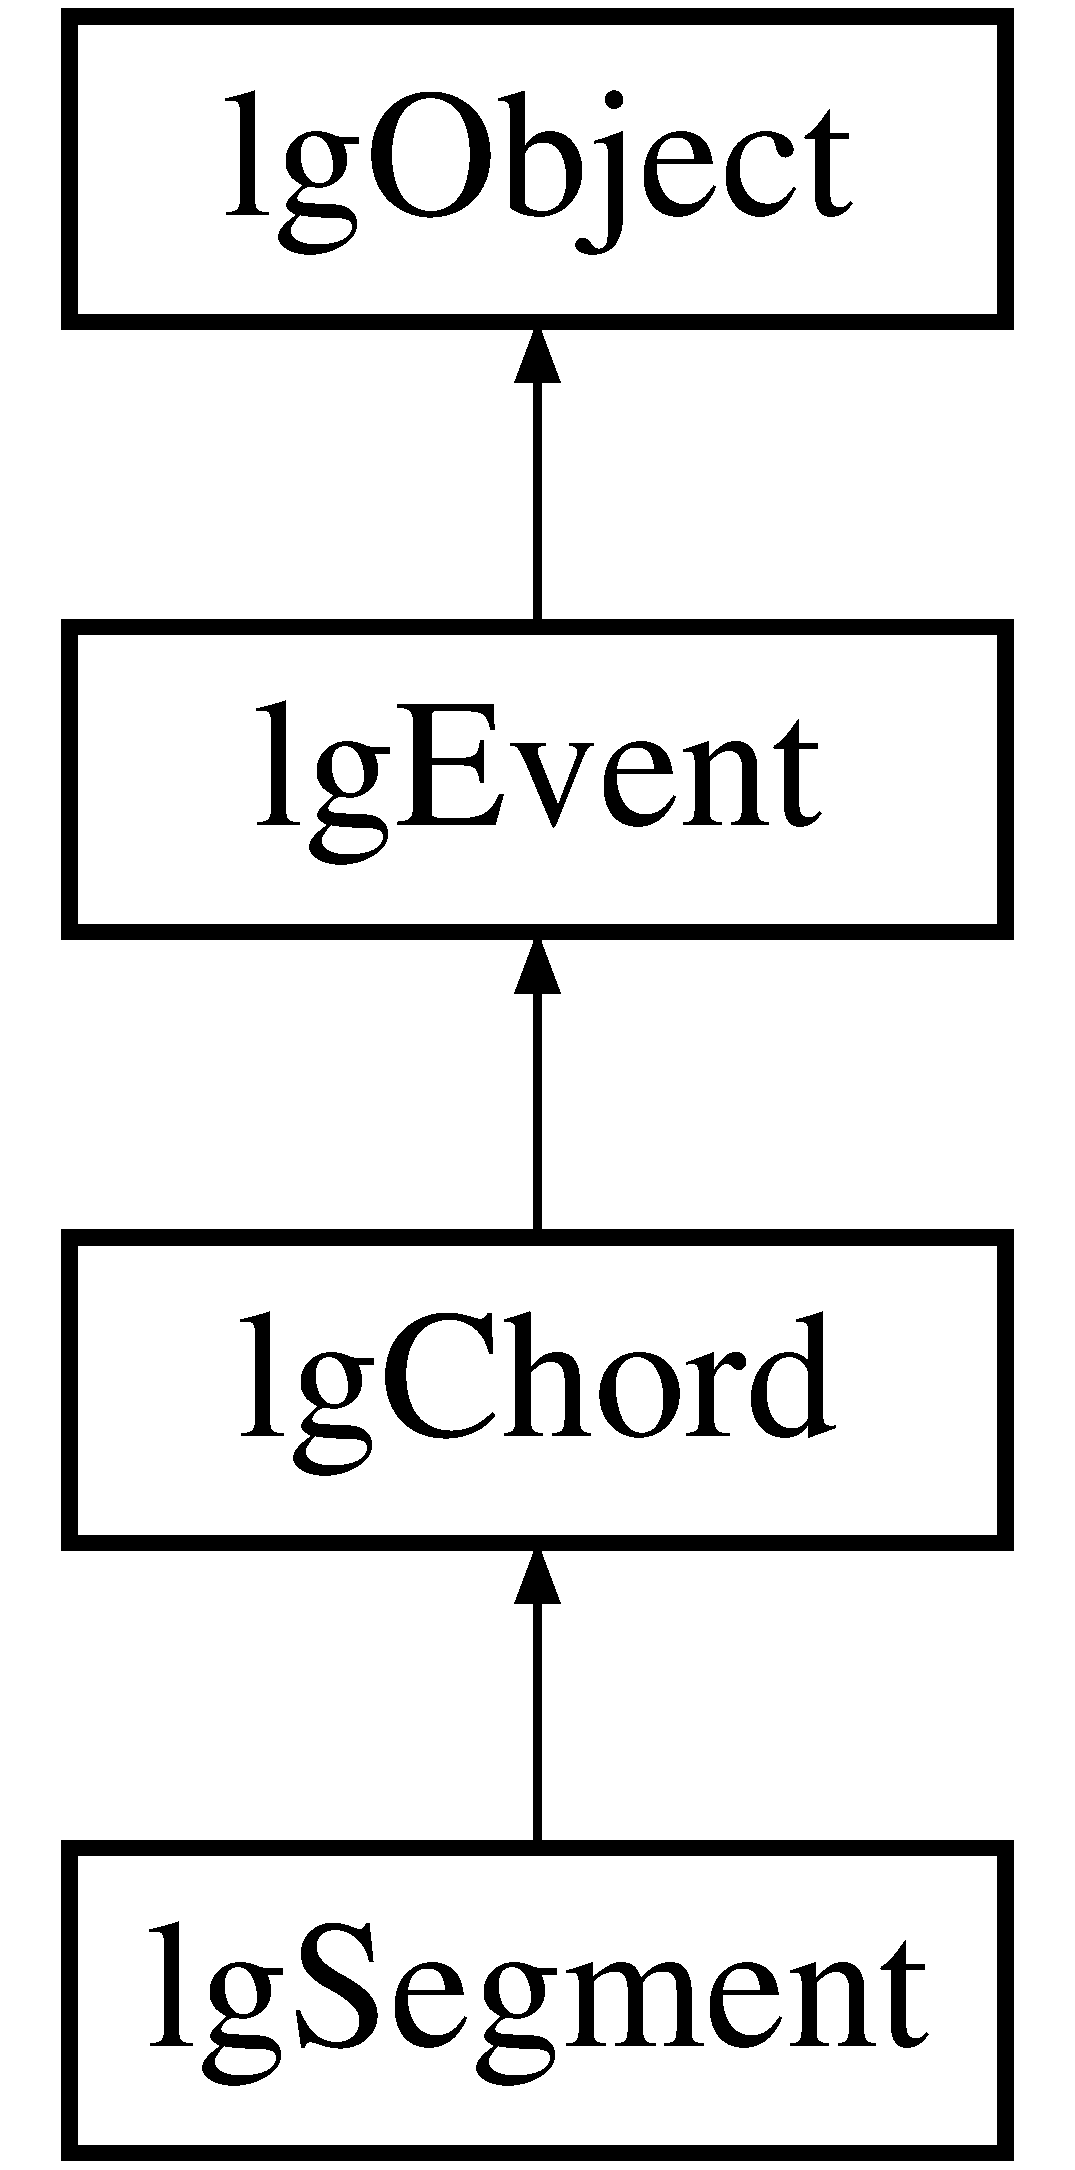
\includegraphics[height=4cm]{classlgChord}
\end{center}
\end{figure}
\subsection*{Public Member Functions}
\begin{CompactItemize}
\item 
void {\bf replace\-Range\-Ptr} ({\bf lg\-Event} $\ast$old, {\bf lg\-Event} $\ast$new\-Ev)
\begin{CompactList}\small\item\em replace in all tags with prev\-Ev\-I==old\-Ev, prev\-Ev by new\-Ev \item\end{CompactList}\item 
{\bf lg\-Chord} (long int pos\-Num, long int pos\-Denom)
\item 
virtual {\bf $\sim$lg\-Chord} (void)
\item 
virtual void {\bf append\-Event} ({\bf lg\-Event} $\ast$ev)
\begin{CompactList}\small\item\em append an event to voices\-Tail \item\end{CompactList}\item 
void {\bf append\-Voice} ({\bf lg\-Voice} $\ast$voice)
\item 
{\bf lg\-Voice} $\ast$ {\bf first\-Voice} (void)
\item 
virtual string {\bf to\-String} ({\bf lg\-Voice} $\ast$call\-Seq)
\begin{CompactList}\small\item\em reset the close\-Range stack for events/tags of all voices \item\end{CompactList}\item 
virtual void {\bf write} (FILE $\ast$out, {\bf lg\-Voice} $\ast$call\-Seq)
\begin{CompactList}\small\item\em write own data AND all tags starting in call\-Seq in (this-$>$pos...next-$>$pos] \item\end{CompactList}\item 
{\bf lg\-Tag} $\ast$ {\bf find\-Tag} (char $\ast$tag\-Name)
\begin{CompactList}\small\item\em search for a tag in all voices \item\end{CompactList}\item 
virtual {\bf lg\-Tag} $\ast$ {\bf find\-Tag} (long int id)
\begin{CompactList}\small\item\em search for a tag in all voices \item\end{CompactList}\item 
int {\bf split\-Tag\-Ranges} (void)
\begin{CompactList}\small\item\em split all explicit tag ranges (using \char`\"{}(....\char`\"{}) ) into $\backslash$...Begin and $\backslash$...End and return number of changed ranges \item\end{CompactList}\end{CompactItemize}
\subsection*{Protected Attributes}
\begin{CompactItemize}
\item 
{\bf lg\-Voice} $\ast$ {\bf voices\-I}
\item 
{\bf lg\-Voice} $\ast$ {\bf voices\-Tail}
\end{CompactItemize}


\subsection{Detailed Description}
a chord based on {\bf lg\-Note}, containing a list of {\bf lg\-Voice} 



\subsection{Constructor \& Destructor Documentation}
\index{lgChord@{lg\-Chord}!lgChord@{lgChord}}
\index{lgChord@{lgChord}!lgChord@{lg\-Chord}}
\subsubsection{\setlength{\rightskip}{0pt plus 5cm}lg\-Chord::lg\-Chord (long int {\em pos\-Num}, long int {\em pos\-Denom})}\label{classlgChord_a1}


\index{lgChord@{lg\-Chord}!~lgChord@{$\sim$lgChord}}
\index{~lgChord@{$\sim$lgChord}!lgChord@{lg\-Chord}}
\subsubsection{\setlength{\rightskip}{0pt plus 5cm}lg\-Chord::$\sim${\bf lg\-Chord} (void)\hspace{0.3cm}{\tt  [virtual]}}\label{classlgChord_a2}




\subsection{Member Function Documentation}
\index{lgChord@{lg\-Chord}!appendEvent@{appendEvent}}
\index{appendEvent@{appendEvent}!lgChord@{lg\-Chord}}
\subsubsection{\setlength{\rightskip}{0pt plus 5cm}void lg\-Chord::append\-Event ({\bf lg\-Event} $\ast$ {\em ev})\hspace{0.3cm}{\tt  [virtual]}}\label{classlgChord_a3}


append an event to voices\-Tail 



Reimplemented in {\bf lg\-Segment} {\rm (p.\,\pageref{classlgSegment_a6})}.\index{lgChord@{lg\-Chord}!appendVoice@{appendVoice}}
\index{appendVoice@{appendVoice}!lgChord@{lg\-Chord}}
\subsubsection{\setlength{\rightskip}{0pt plus 5cm}void lg\-Chord::append\-Voice ({\bf lg\-Voice} $\ast$ {\em v})}\label{classlgChord_a4}


append voice to chord, voices\-Tail must be up to date! \begin{Desc}
\item[Parameters: ]\par
\begin{description}
\item[{\em 
v}]sequence or voice \end{description}
\end{Desc}
\index{lgChord@{lg\-Chord}!findTag@{findTag}}
\index{findTag@{findTag}!lgChord@{lg\-Chord}}
\subsubsection{\setlength{\rightskip}{0pt plus 5cm}{\bf lg\-Tag} $\ast$ lg\-Chord::find\-Tag (long int {\em id})\hspace{0.3cm}{\tt  [virtual]}}\label{classlgChord_a9}


search for a tag in all voices 

\index{lgChord@{lg\-Chord}!findTag@{findTag}}
\index{findTag@{findTag}!lgChord@{lg\-Chord}}
\subsubsection{\setlength{\rightskip}{0pt plus 5cm}{\bf lg\-Tag} $\ast$ lg\-Chord::find\-Tag (char $\ast$ {\em tag\-Name})}\label{classlgChord_a8}


search for a tag in all voices 

\index{lgChord@{lg\-Chord}!firstVoice@{firstVoice}}
\index{firstVoice@{firstVoice}!lgChord@{lg\-Chord}}
\subsubsection{\setlength{\rightskip}{0pt plus 5cm}{\bf lg\-Voice}$\ast$ lg\-Chord::first\-Voice (void)\hspace{0.3cm}{\tt  [inline]}}\label{classlgChord_a5}


\index{lgChord@{lg\-Chord}!replaceRangePtr@{replaceRangePtr}}
\index{replaceRangePtr@{replaceRangePtr}!lgChord@{lg\-Chord}}
\subsubsection{\setlength{\rightskip}{0pt plus 5cm}void lg\-Chord::replace\-Range\-Ptr ({\bf lg\-Event} $\ast$ {\em old}, {\bf lg\-Event} $\ast$ {\em new\-Ev})}\label{classlgChord_a0}


replace in all tags with prev\-Ev\-I==old\-Ev, prev\-Ev by new\-Ev 

\index{lgChord@{lg\-Chord}!splitTagRanges@{splitTagRanges}}
\index{splitTagRanges@{splitTagRanges}!lgChord@{lg\-Chord}}
\subsubsection{\setlength{\rightskip}{0pt plus 5cm}int lg\-Chord::split\-Tag\-Ranges (void)}\label{classlgChord_a10}


split all explicit tag ranges (using \char`\"{}(....\char`\"{}) ) into $\backslash$...Begin and $\backslash$...End and return number of changed ranges 

\index{lgChord@{lg\-Chord}!toString@{toString}}
\index{toString@{toString}!lgChord@{lg\-Chord}}
\subsubsection{\setlength{\rightskip}{0pt plus 5cm}string lg\-Chord::to\-String ({\bf lg\-Voice} $\ast$ {\em call\-Seq})\hspace{0.3cm}{\tt  [virtual]}}\label{classlgChord_a6}


reset the close\-Range stack for events/tags of all voices 

write all tags between this and next call\-Seq might be NULL for Segements 

Reimplemented from {\bf lg\-Event} {\rm (p.\,\pageref{classlgEvent_a1})}.

Reimplemented in {\bf lg\-Segment} {\rm (p.\,\pageref{classlgSegment_a21})}.\index{lgChord@{lg\-Chord}!write@{write}}
\index{write@{write}!lgChord@{lg\-Chord}}
\subsubsection{\setlength{\rightskip}{0pt plus 5cm}void lg\-Chord::write (FILE $\ast$ {\em out}, {\bf lg\-Voice} $\ast$ {\em call\-Seq})\hspace{0.3cm}{\tt  [virtual]}}\label{classlgChord_a7}


write own data AND all tags starting in call\-Seq in (this-$>$pos...next-$>$pos] 



Reimplemented from {\bf lg\-Event} {\rm (p.\,\pageref{classlgEvent_a8})}.

Reimplemented in {\bf lg\-Segment} {\rm (p.\,\pageref{classlgSegment_a22})}.

\subsection{Member Data Documentation}
\index{lgChord@{lg\-Chord}!voicesI@{voicesI}}
\index{voicesI@{voicesI}!lgChord@{lg\-Chord}}
\subsubsection{\setlength{\rightskip}{0pt plus 5cm}{\bf lg\-Voice}$\ast$ {\bf lg\-Chord::voices\-I}\hspace{0.3cm}{\tt  [protected]}}\label{classlgChord_p0}


\index{lgChord@{lg\-Chord}!voicesTail@{voicesTail}}
\index{voicesTail@{voicesTail}!lgChord@{lg\-Chord}}
\subsubsection{\setlength{\rightskip}{0pt plus 5cm}{\bf lg\-Voice} $\ast$ {\bf lg\-Chord::voices\-Tail}\hspace{0.3cm}{\tt  [protected]}}\label{classlgChord_p1}




The documentation for this class was generated from the following files:\begin{CompactItemize}
\item 
{\bf lgchord.h}\item 
{\bf lgchord.cpp}\end{CompactItemize}

\section{lg\-Duration Class Reference}
\label{classlgDuration}\index{lgDuration@{lgDuration}}
generic fraction class. lg\-Duration is used to store the information pertaining to the duration/attacktime of a note.  


{\tt \#include $<$duration.h$>$}

\subsection*{Public Member Functions}
\begin{CompactItemize}
\item 
{\bf lg\-Duration} (long int num=0, long int denom=1)
\item 
{\bf lg\-Duration} (const {\bf lg\-Duration} \&d)
\item 
{\bf lg\-Duration} (const string \&str)
\item 
{\bf lg\-Duration} {\bf operator+} (const {\bf lg\-Duration} \&dur)
\item 
{\bf lg\-Duration} {\bf operator-} (const {\bf lg\-Duration} \&dur)
\item 
{\bf lg\-Duration} {\bf operator $\ast$} (const {\bf lg\-Duration} \&dur)
\begin{CompactList}\small\item\em Useful for notes with dots. \item\end{CompactList}\item 
{\bf lg\-Duration} {\bf operator/} (const {\bf lg\-Duration} \&dur)
\item 
{\bf lg\-Duration} \& {\bf operator+=} (const {\bf lg\-Duration} \&dur)
\item 
{\bf lg\-Duration} \& {\bf operator-=} (const {\bf lg\-Duration} \&dur)
\item 
{\bf lg\-Duration} \& {\bf operator $\ast$=} (const {\bf lg\-Duration} \&dur)
\begin{CompactList}\small\item\em Useful for notes with dots. \item\end{CompactList}\item 
{\bf lg\-Duration} \& {\bf operator/=} (const {\bf lg\-Duration} \&dur)
\item 
bool {\bf operator$>$} (const {\bf lg\-Duration} \&dur)
\item 
bool {\bf operator$>$=} (const {\bf lg\-Duration} \&dur)
\item 
bool {\bf operator$<$} (const {\bf lg\-Duration} \&dur)
\item 
bool {\bf operator$<$=} (const {\bf lg\-Duration} \&dur)
\item 
bool {\bf operator==} (const {\bf lg\-Duration} \&dur)
\item 
bool {\bf operator!=} (const {\bf lg\-Duration} \&dur)
\item 
void {\bf rationalise} (void)
\begin{CompactList}\small\item\em Used to \char`\"{}rationalise\char`\"{} duration. \item\end{CompactList}\item 
long int {\bf gcd} (long int a, long int b)
\begin{CompactList}\small\item\em Used by {\bf rationalise()}. greatest common divisor. \item\end{CompactList}\item 
virtual string {\bf to\-String} (void)
\item 
void {\bf write} (FILE $\ast$out)
\item 
double {\bf to\-Double} (void)
\end{CompactItemize}
\subsection*{Public Attributes}
\begin{CompactItemize}
\item 
long int {\bf dur\-N}
\begin{CompactList}\small\item\em numerator \item\end{CompactList}\item 
long int {\bf dur\-D}
\begin{CompactList}\small\item\em denominator \item\end{CompactList}\end{CompactItemize}


\subsection{Detailed Description}
generic fraction class. lg\-Duration is used to store the information pertaining to the duration/attacktime of a note. 



\subsection{Constructor \& Destructor Documentation}
\index{lgDuration@{lg\-Duration}!lgDuration@{lgDuration}}
\index{lgDuration@{lgDuration}!lgDuration@{lg\-Duration}}
\subsubsection{\setlength{\rightskip}{0pt plus 5cm}lg\-Duration::lg\-Duration (long int {\em num} = 0, long int {\em denom} = 1)}\label{classlgDuration_a0}


\index{lgDuration@{lg\-Duration}!lgDuration@{lgDuration}}
\index{lgDuration@{lgDuration}!lgDuration@{lg\-Duration}}
\subsubsection{\setlength{\rightskip}{0pt plus 5cm}lg\-Duration::lg\-Duration (const {\bf lg\-Duration} \& {\em d})}\label{classlgDuration_a1}


\index{lgDuration@{lg\-Duration}!lgDuration@{lgDuration}}
\index{lgDuration@{lgDuration}!lgDuration@{lg\-Duration}}
\subsubsection{\setlength{\rightskip}{0pt plus 5cm}lg\-Duration::lg\-Duration (const string \& {\em str})}\label{classlgDuration_a2}




\subsection{Member Function Documentation}
\index{lgDuration@{lg\-Duration}!gcd@{gcd}}
\index{gcd@{gcd}!lgDuration@{lg\-Duration}}
\subsubsection{\setlength{\rightskip}{0pt plus 5cm}long int lg\-Duration::gcd (long int {\em a}, long int {\em b})}\label{classlgDuration_a18}


Used by {\bf rationalise()}. greatest common divisor. 

\index{lgDuration@{lg\-Duration}!operator *@{operator $\ast$}}
\index{operator *@{operator $\ast$}!lgDuration@{lg\-Duration}}
\subsubsection{\setlength{\rightskip}{0pt plus 5cm}{\bf lg\-Duration} lg\-Duration::operator $\ast$ (const {\bf lg\-Duration} \& {\em dur})}\label{classlgDuration_a5}


Useful for notes with dots. 

\index{lgDuration@{lg\-Duration}!operator *=@{operator $\ast$=}}
\index{operator *=@{operator $\ast$=}!lgDuration@{lg\-Duration}}
\subsubsection{\setlength{\rightskip}{0pt plus 5cm}{\bf lg\-Duration} \& lg\-Duration::operator $\ast$= (const {\bf lg\-Duration} \& {\em dur})}\label{classlgDuration_a9}


Useful for notes with dots. 

\index{lgDuration@{lg\-Duration}!operator"!=@{operator"!=}}
\index{operator"!=@{operator"!=}!lgDuration@{lg\-Duration}}
\subsubsection{\setlength{\rightskip}{0pt plus 5cm}bool lg\-Duration::operator!= (const {\bf lg\-Duration} \& {\em dur})}\label{classlgDuration_a16}


\index{lgDuration@{lg\-Duration}!operator+@{operator+}}
\index{operator+@{operator+}!lgDuration@{lg\-Duration}}
\subsubsection{\setlength{\rightskip}{0pt plus 5cm}{\bf lg\-Duration} lg\-Duration::operator+ (const {\bf lg\-Duration} \& {\em dur})}\label{classlgDuration_a3}


\index{lgDuration@{lg\-Duration}!operator+=@{operator+=}}
\index{operator+=@{operator+=}!lgDuration@{lg\-Duration}}
\subsubsection{\setlength{\rightskip}{0pt plus 5cm}{\bf lg\-Duration} \& lg\-Duration::operator+= (const {\bf lg\-Duration} \& {\em dur})}\label{classlgDuration_a7}


\index{lgDuration@{lg\-Duration}!operator-@{operator-}}
\index{operator-@{operator-}!lgDuration@{lg\-Duration}}
\subsubsection{\setlength{\rightskip}{0pt plus 5cm}{\bf lg\-Duration} lg\-Duration::operator- (const {\bf lg\-Duration} \& {\em dur})}\label{classlgDuration_a4}


\index{lgDuration@{lg\-Duration}!operator-=@{operator-=}}
\index{operator-=@{operator-=}!lgDuration@{lg\-Duration}}
\subsubsection{\setlength{\rightskip}{0pt plus 5cm}{\bf lg\-Duration} \& lg\-Duration::operator-= (const {\bf lg\-Duration} \& {\em dur})}\label{classlgDuration_a8}


\index{lgDuration@{lg\-Duration}!operator/@{operator/}}
\index{operator/@{operator/}!lgDuration@{lg\-Duration}}
\subsubsection{\setlength{\rightskip}{0pt plus 5cm}{\bf lg\-Duration} lg\-Duration::operator/ (const {\bf lg\-Duration} \& {\em dur})}\label{classlgDuration_a6}


\index{lgDuration@{lg\-Duration}!operator/=@{operator/=}}
\index{operator/=@{operator/=}!lgDuration@{lg\-Duration}}
\subsubsection{\setlength{\rightskip}{0pt plus 5cm}{\bf lg\-Duration} \& lg\-Duration::operator/= (const {\bf lg\-Duration} \& {\em dur})}\label{classlgDuration_a10}


\index{lgDuration@{lg\-Duration}!operator<@{operator$<$}}
\index{operator<@{operator$<$}!lgDuration@{lg\-Duration}}
\subsubsection{\setlength{\rightskip}{0pt plus 5cm}bool lg\-Duration::operator$<$ (const {\bf lg\-Duration} \& {\em dur})}\label{classlgDuration_a13}


\index{lgDuration@{lg\-Duration}!operator<=@{operator$<$=}}
\index{operator<=@{operator$<$=}!lgDuration@{lg\-Duration}}
\subsubsection{\setlength{\rightskip}{0pt plus 5cm}bool lg\-Duration::operator$<$= (const {\bf lg\-Duration} \& {\em dur})\hspace{0.3cm}{\tt  [inline]}}\label{classlgDuration_a14}


\index{lgDuration@{lg\-Duration}!operator==@{operator==}}
\index{operator==@{operator==}!lgDuration@{lg\-Duration}}
\subsubsection{\setlength{\rightskip}{0pt plus 5cm}bool lg\-Duration::operator== (const {\bf lg\-Duration} \& {\em dur})}\label{classlgDuration_a15}


\index{lgDuration@{lg\-Duration}!operator>@{operator$>$}}
\index{operator>@{operator$>$}!lgDuration@{lg\-Duration}}
\subsubsection{\setlength{\rightskip}{0pt plus 5cm}bool lg\-Duration::operator$>$ (const {\bf lg\-Duration} \& {\em dur})}\label{classlgDuration_a11}


\index{lgDuration@{lg\-Duration}!operator>=@{operator$>$=}}
\index{operator>=@{operator$>$=}!lgDuration@{lg\-Duration}}
\subsubsection{\setlength{\rightskip}{0pt plus 5cm}bool lg\-Duration::operator$>$= (const {\bf lg\-Duration} \& {\em dur})\hspace{0.3cm}{\tt  [inline]}}\label{classlgDuration_a12}


\index{lgDuration@{lg\-Duration}!rationalise@{rationalise}}
\index{rationalise@{rationalise}!lgDuration@{lg\-Duration}}
\subsubsection{\setlength{\rightskip}{0pt plus 5cm}void lg\-Duration::rationalise (void)}\label{classlgDuration_a17}


Used to \char`\"{}rationalise\char`\"{} duration. 

\index{lgDuration@{lg\-Duration}!toDouble@{toDouble}}
\index{toDouble@{toDouble}!lgDuration@{lg\-Duration}}
\subsubsection{\setlength{\rightskip}{0pt plus 5cm}double lg\-Duration::to\-Double (void)}\label{classlgDuration_a21}


\index{lgDuration@{lg\-Duration}!toString@{toString}}
\index{toString@{toString}!lgDuration@{lg\-Duration}}
\subsubsection{\setlength{\rightskip}{0pt plus 5cm}string lg\-Duration::to\-String (void)\hspace{0.3cm}{\tt  [virtual]}}\label{classlgDuration_a19}


\index{lgDuration@{lg\-Duration}!write@{write}}
\index{write@{write}!lgDuration@{lg\-Duration}}
\subsubsection{\setlength{\rightskip}{0pt plus 5cm}void lg\-Duration::write (FILE $\ast$ {\em out})}\label{classlgDuration_a20}




\subsection{Member Data Documentation}
\index{lgDuration@{lg\-Duration}!durD@{durD}}
\index{durD@{durD}!lgDuration@{lg\-Duration}}
\subsubsection{\setlength{\rightskip}{0pt plus 5cm}long int {\bf lg\-Duration::dur\-D}}\label{classlgDuration_o1}


denominator 

\index{lgDuration@{lg\-Duration}!durN@{durN}}
\index{durN@{durN}!lgDuration@{lg\-Duration}}
\subsubsection{\setlength{\rightskip}{0pt plus 5cm}long int {\bf lg\-Duration::dur\-N}}\label{classlgDuration_o0}


numerator 



The documentation for this class was generated from the following files:\begin{CompactItemize}
\item 
{\bf duration.h}\item 
{\bf duration.cpp}\end{CompactItemize}

\section{lg\-Empty Class Reference}
\label{classlgEmpty}\index{lgEmpty@{lgEmpty}}
empty note based on {\bf lg\-Note} see GUIDO spec for description  


{\tt \#include $<$lgempty.h$>$}

Inheritance diagram for lg\-Empty::\begin{figure}[H]
\begin{center}
\leavevmode
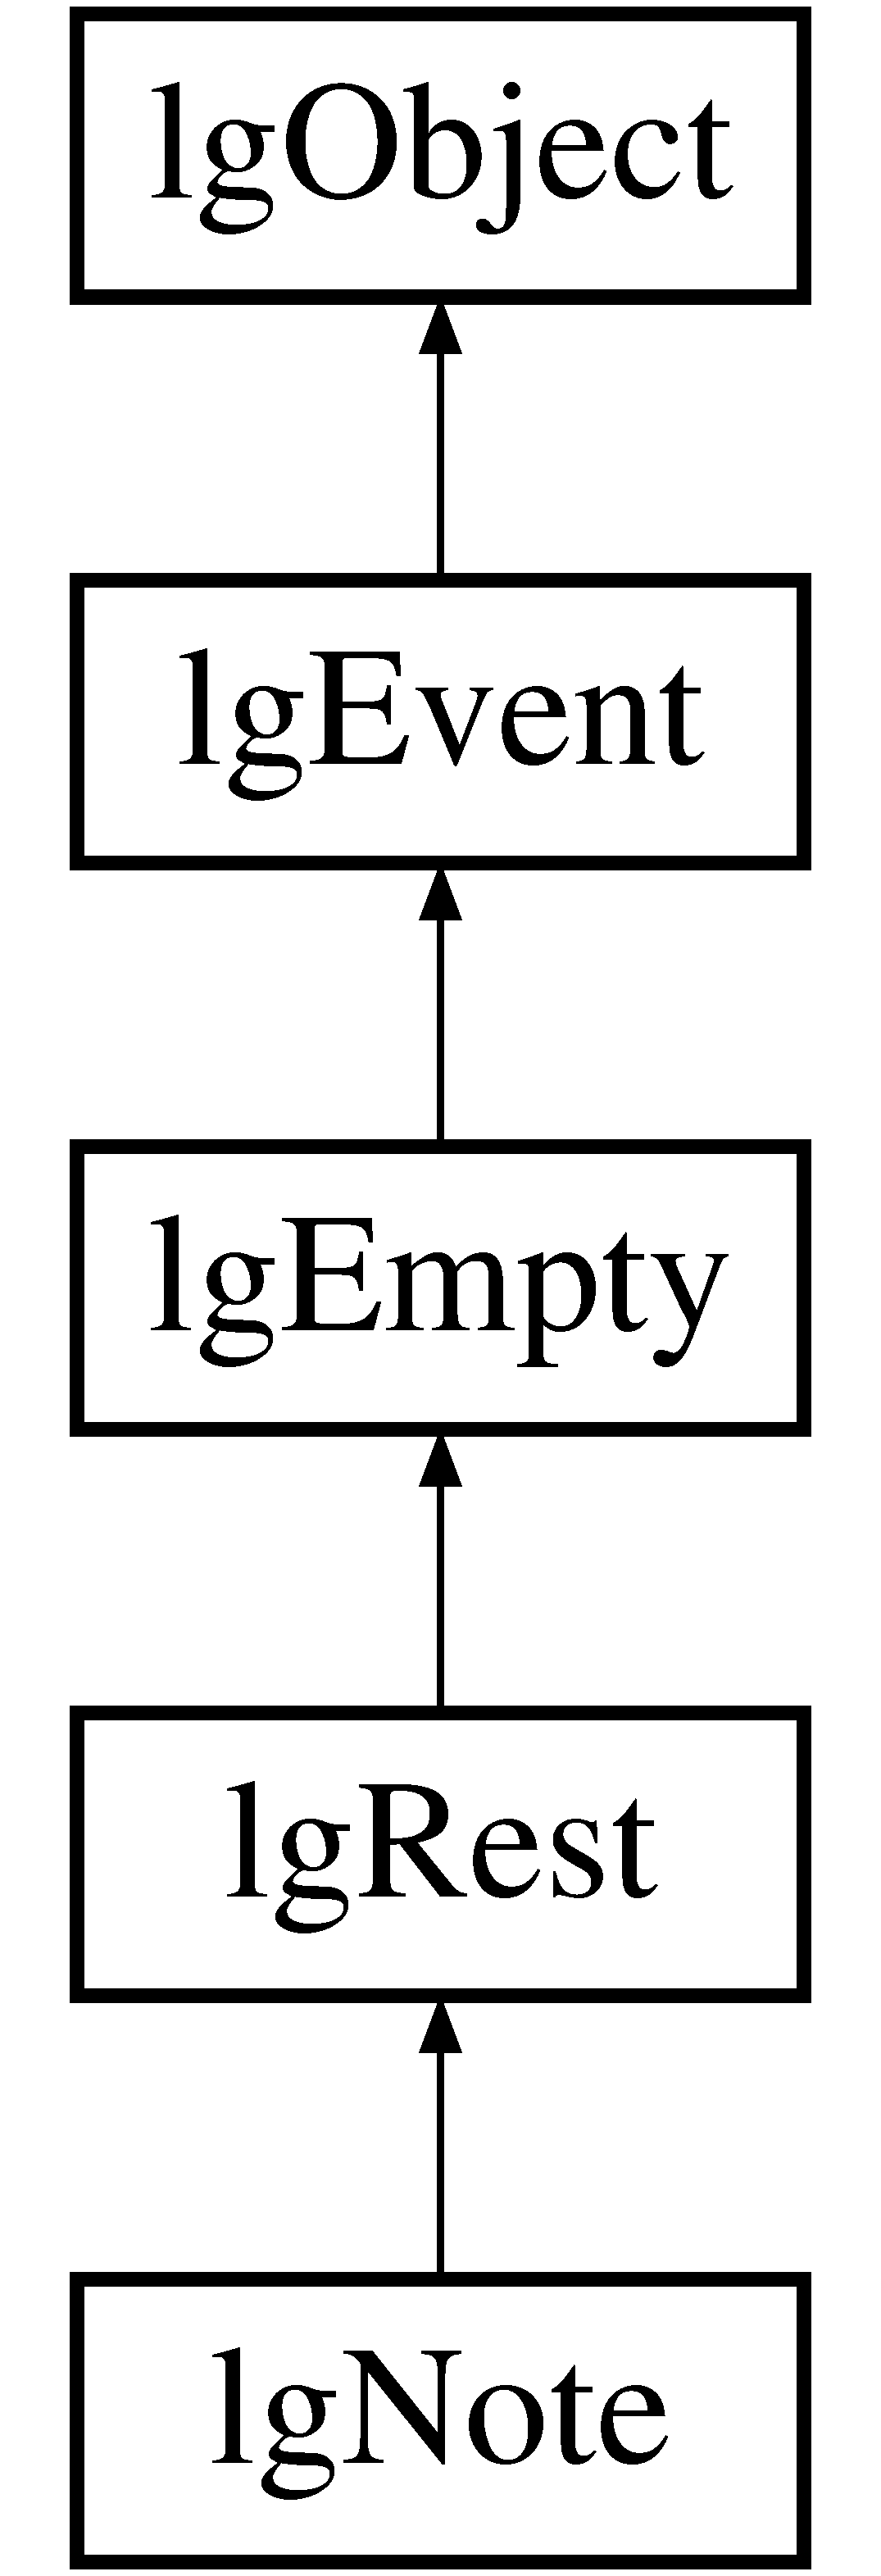
\includegraphics[height=5cm]{classlgEmpty}
\end{center}
\end{figure}
\subsection*{Public Member Functions}
\begin{CompactItemize}
\item 
virtual string {\bf to\-String} ({\bf lg\-Voice} $\ast$calling\-Seq=NULL)
\begin{CompactList}\small\item\em write \char`\"{}empty\char`\"{} \item\end{CompactList}\item 
{\bf lg\-Empty} (long int dur\-Num, long int dur\-Denom, int cdots, long int pos\-Num, long int pos\-Denom)
\end{CompactItemize}


\subsection{Detailed Description}
empty note based on {\bf lg\-Note} see GUIDO spec for description 



\subsection{Constructor \& Destructor Documentation}
\index{lgEmpty@{lg\-Empty}!lgEmpty@{lgEmpty}}
\index{lgEmpty@{lgEmpty}!lgEmpty@{lg\-Empty}}
\subsubsection{\setlength{\rightskip}{0pt plus 5cm}lg\-Empty::lg\-Empty (long int {\em dur\-Num}, long int {\em dur\-Denom}, int {\em cdots}, long int {\em pos\-Num}, long int {\em pos\-Denom})}\label{classlgEmpty_a1}




\subsection{Member Function Documentation}
\index{lgEmpty@{lg\-Empty}!toString@{toString}}
\index{toString@{toString}!lgEmpty@{lg\-Empty}}
\subsubsection{\setlength{\rightskip}{0pt plus 5cm}string lg\-Empty::to\-String ({\bf lg\-Voice} $\ast$ {\em calling\-Seq} = NULL)\hspace{0.3cm}{\tt  [virtual]}}\label{classlgEmpty_a0}


write \char`\"{}empty\char`\"{} 



Reimplemented from {\bf lg\-Event} {\rm (p.\,\pageref{classlgEvent_a1})}.

Reimplemented in {\bf lg\-Note} {\rm (p.\,\pageref{classlgNote_a0})}, and {\bf lg\-Rest} {\rm (p.\,\pageref{classlgRest_a0})}.

The documentation for this class was generated from the following files:\begin{CompactItemize}
\item 
{\bf lgempty.h}\item 
{\bf lgempty.cpp}\end{CompactItemize}

\section{lg\-Event Class Reference}
\label{classlgEvent}\index{lgEvent@{lgEvent}}
A {\bf lg\-Object} with duration and time-position.  


{\tt \#include $<$lgevent.h$>$}

Inheritance diagram for lg\-Event::\begin{figure}[H]
\begin{center}
\leavevmode
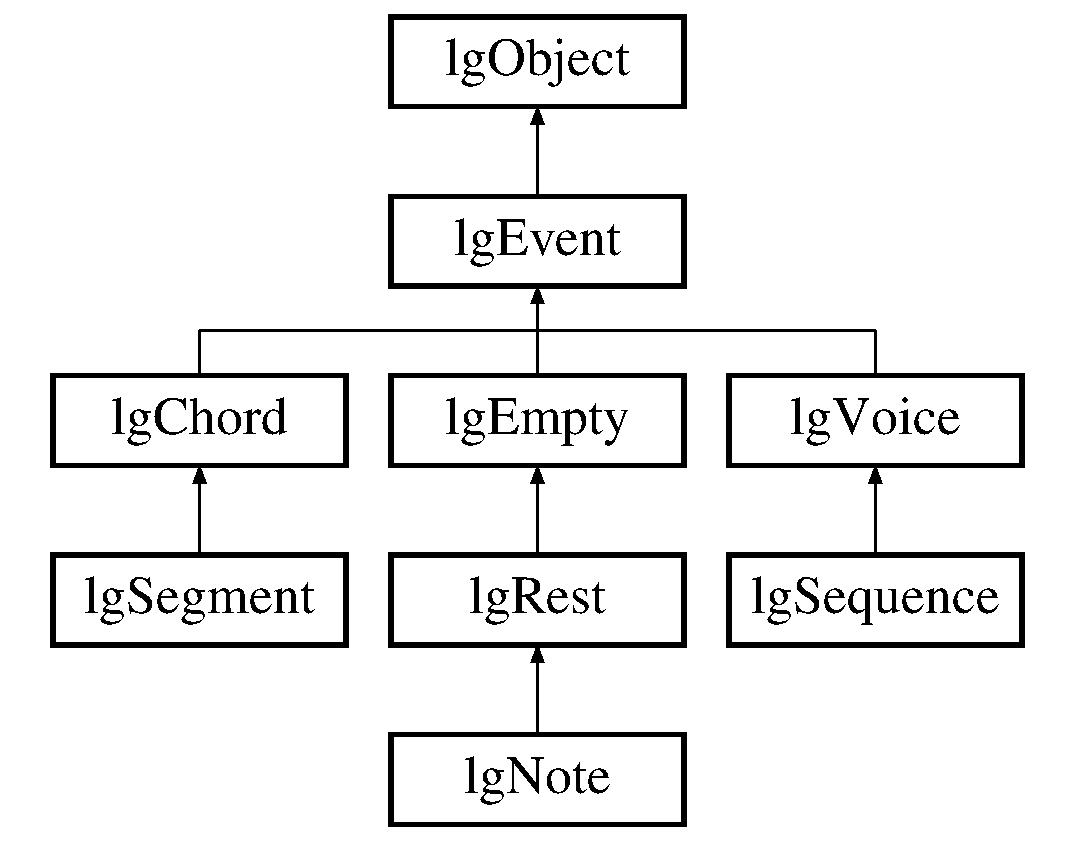
\includegraphics[height=5cm]{classlgEvent}
\end{center}
\end{figure}
\subsection*{Public Member Functions}
\begin{CompactItemize}
\item 
{\bf lg\-Event} (long int dur\-Num, long int dur\-Denom, int cdots, long int pos\-Num, long int pos\-Denom)
\item 
virtual string {\bf to\-String} ({\bf lg\-Voice} $\ast$calling\-Seq=NULL)
\begin{CompactList}\small\item\em lg\-Event returns only the duration as a string \item\end{CompactList}\item 
virtual lg\-Frac {\bf duration} (void)
\begin{CompactList}\small\item\em duration of event including c\-Dot info! \item\end{CompactList}\item 
virtual lg\-Frac {\bf head\-Duration} (void)
\begin{CompactList}\small\item\em return only explicite written duration without dots, is zero for lg\-Voice! \item\end{CompactList}\item 
int {\bf c\-Dots} (void)
\begin{CompactList}\small\item\em number of written dots \item\end{CompactList}\item 
virtual void {\bf set\-Duration} ({\bf lg\-Duration} dur, int dots=0)
\begin{CompactList}\small\item\em set the duration \item\end{CompactList}\item 
virtual lg\-Frac {\bf pos} (void)
\begin{CompactList}\small\item\em absolute time position. needs to be updated if previous events were inserted or deleted! \item\end{CompactList}\item 
virtual void {\bf set\-Pos} (const lg\-Frac \&pos)
\begin{CompactList}\small\item\em be carefull that list is consistent! \item\end{CompactList}\item 
virtual void {\bf write} (FILE $\ast$out, {\bf lg\-Voice} $\ast$call\-Seq)
\begin{CompactList}\small\item\em write own data AND all tags starting in call\-Seq in (this-$>$pos...next-$>$pos] \item\end{CompactList}\item 
{\bf lg\-Note} $\ast$ {\bf next\-Note} (void)
\begin{CompactList}\small\item\em skip all rests, etc. \item\end{CompactList}\end{CompactItemize}
\subsection*{Protected Member Functions}
\begin{CompactItemize}
\item 
virtual void {\bf write\-V} (FILE $\ast$out)
\end{CompactItemize}
\subsection*{Private Attributes}
\begin{CompactItemize}
\item 
{\bf lg\-Duration} {\bf pos\-I}
\begin{CompactList}\small\item\em time position of event, events of a voice must not overlap each other! \item\end{CompactList}\item 
{\bf lg\-Duration} {\bf duration\-I}
\begin{CompactList}\small\item\em the \char`\"{}written\char`\"{} duration excluding dots (= duration of notehead)! \item\end{CompactList}\item 
long int {\bf c\-Dots\-I}
\begin{CompactList}\small\item\em the number of dots \item\end{CompactList}\end{CompactItemize}
\subsection*{Friends}
\begin{CompactItemize}
\item 
class {\bf lg\-Voice}
\begin{CompactList}\small\item\em needs access to set\-Next \item\end{CompactList}\item 
class {\bf lg\-Chord}
\begin{CompactList}\small\item\em needs access to set\-Next \item\end{CompactList}\end{CompactItemize}


\subsection{Detailed Description}
A {\bf lg\-Object} with duration and time-position. 



\subsection{Constructor \& Destructor Documentation}
\index{lgEvent@{lg\-Event}!lgEvent@{lgEvent}}
\index{lgEvent@{lgEvent}!lgEvent@{lg\-Event}}
\subsubsection{\setlength{\rightskip}{0pt plus 5cm}lg\-Event::lg\-Event (long int {\em dur\-Num}, long int {\em dur\-Denom}, int {\em cdots}, long int {\em pos\-Num}, long int {\em pos\-Denom})}\label{classlgEvent_a0}


close range\-Stack gives the number of \char`\"{})\char`\"{} which should be placed after \char`\"{}this\char`\"{} in the .gmn out. If any tag or note is added/removed to/from the tag/note list, close\-Range needs to be updated -$>$ see {\bf lg\-Voice} 

\subsection{Member Function Documentation}
\index{lgEvent@{lg\-Event}!cDots@{cDots}}
\index{cDots@{cDots}!lgEvent@{lg\-Event}}
\subsubsection{\setlength{\rightskip}{0pt plus 5cm}int lg\-Event::c\-Dots (void)\hspace{0.3cm}{\tt  [inline]}}\label{classlgEvent_a4}


number of written dots 

\index{lgEvent@{lg\-Event}!duration@{duration}}
\index{duration@{duration}!lgEvent@{lg\-Event}}
\subsubsection{\setlength{\rightskip}{0pt plus 5cm}{\bf lg\-Duration} lg\-Event::duration (void)\hspace{0.3cm}{\tt  [virtual]}}\label{classlgEvent_a2}


duration of event including c\-Dot info! 



Reimplemented in {\bf lg\-Voice} {\rm (p.\,\pageref{classlgVoice_a22})}.\index{lgEvent@{lg\-Event}!headDuration@{headDuration}}
\index{headDuration@{headDuration}!lgEvent@{lg\-Event}}
\subsubsection{\setlength{\rightskip}{0pt plus 5cm}virtual lg\-Frac lg\-Event::head\-Duration (void)\hspace{0.3cm}{\tt  [inline, virtual]}}\label{classlgEvent_a3}


return only explicite written duration without dots, is zero for lg\-Voice! 

\index{lgEvent@{lg\-Event}!nextNote@{nextNote}}
\index{nextNote@{nextNote}!lgEvent@{lg\-Event}}
\subsubsection{\setlength{\rightskip}{0pt plus 5cm}{\bf lg\-Note} $\ast$ lg\-Event::next\-Note (void)}\label{classlgEvent_a9}


skip all rests, etc. 

\index{lgEvent@{lg\-Event}!pos@{pos}}
\index{pos@{pos}!lgEvent@{lg\-Event}}
\subsubsection{\setlength{\rightskip}{0pt plus 5cm}virtual lg\-Frac lg\-Event::pos (void)\hspace{0.3cm}{\tt  [inline, virtual]}}\label{classlgEvent_a6}


absolute time position. needs to be updated if previous events were inserted or deleted! 



Reimplemented from {\bf lg\-Object} {\rm (p.\,\pageref{classlgObject_a5})}.\index{lgEvent@{lg\-Event}!setDuration@{setDuration}}
\index{setDuration@{setDuration}!lgEvent@{lg\-Event}}
\subsubsection{\setlength{\rightskip}{0pt plus 5cm}virtual void lg\-Event::set\-Duration ({\bf lg\-Duration} {\em dur}, int {\em dots} = 0)\hspace{0.3cm}{\tt  [inline, virtual]}}\label{classlgEvent_a5}


set the duration 

\index{lgEvent@{lg\-Event}!setPos@{setPos}}
\index{setPos@{setPos}!lgEvent@{lg\-Event}}
\subsubsection{\setlength{\rightskip}{0pt plus 5cm}virtual void lg\-Event::set\-Pos (const lg\-Frac \& {\em pos})\hspace{0.3cm}{\tt  [inline, virtual]}}\label{classlgEvent_a7}


be carefull that list is consistent! 

\index{lgEvent@{lg\-Event}!toString@{toString}}
\index{toString@{toString}!lgEvent@{lg\-Event}}
\subsubsection{\setlength{\rightskip}{0pt plus 5cm}string lg\-Event::to\-String ({\bf lg\-Voice} $\ast$ {\em calling\-Seq} = NULL)\hspace{0.3cm}{\tt  [virtual]}}\label{classlgEvent_a1}


lg\-Event returns only the duration as a string 



Reimplemented from {\bf lg\-Object} {\rm (p.\,\pageref{classlgObject_a3})}.

Reimplemented in {\bf lg\-Chord} {\rm (p.\,\pageref{classlgChord_a6})}, {\bf lg\-Empty} {\rm (p.\,\pageref{classlgEmpty_a0})}, {\bf lg\-Note} {\rm (p.\,\pageref{classlgNote_a0})}, {\bf lg\-Rest} {\rm (p.\,\pageref{classlgRest_a0})}, {\bf lg\-Segment} {\rm (p.\,\pageref{classlgSegment_a21})}, {\bf lg\-Sequence} {\rm (p.\,\pageref{classlgSequence_a0})}, and {\bf lg\-Voice} {\rm (p.\,\pageref{classlgVoice_a20})}.\index{lgEvent@{lg\-Event}!write@{write}}
\index{write@{write}!lgEvent@{lg\-Event}}
\subsubsection{\setlength{\rightskip}{0pt plus 5cm}void lg\-Event::write (FILE $\ast$ {\em out}, {\bf lg\-Voice} $\ast$ {\em call\-Seq})\hspace{0.3cm}{\tt  [virtual]}}\label{classlgEvent_a8}


write own data AND all tags starting in call\-Seq in (this-$>$pos...next-$>$pos] 



Reimplemented from {\bf lg\-Object} {\rm (p.\,\pageref{classlgObject_a4})}.

Reimplemented in {\bf lg\-Chord} {\rm (p.\,\pageref{classlgChord_a7})}, {\bf lg\-Segment} {\rm (p.\,\pageref{classlgSegment_a22})}, and {\bf lg\-Voice} {\rm (p.\,\pageref{classlgVoice_a21})}.\index{lgEvent@{lg\-Event}!writeV@{writeV}}
\index{writeV@{writeV}!lgEvent@{lg\-Event}}
\subsubsection{\setlength{\rightskip}{0pt plus 5cm}virtual void lg\-Event::write\-V (FILE $\ast$ {\em out})\hspace{0.3cm}{\tt  [inline, protected, virtual]}}\label{classlgEvent_b0}


should be overwritten in derived classes write class spec values (pitch, \_\-, ..) 

\subsection{Friends And Related Function Documentation}
\index{lgEvent@{lg\-Event}!lgChord@{lgChord}}
\index{lgChord@{lgChord}!lgEvent@{lg\-Event}}
\subsubsection{\setlength{\rightskip}{0pt plus 5cm}friend class {\bf lg\-Chord}\hspace{0.3cm}{\tt  [friend]}}\label{classlgEvent_n1}


needs access to set\-Next 



Reimplemented from {\bf lg\-Object} {\rm (p.\,\pageref{classlgObject_n5})}.

Reimplemented in {\bf lg\-Voice} {\rm (p.\,\pageref{classlgVoice_n0})}.\index{lgEvent@{lg\-Event}!lgVoice@{lgVoice}}
\index{lgVoice@{lgVoice}!lgEvent@{lg\-Event}}
\subsubsection{\setlength{\rightskip}{0pt plus 5cm}friend class {\bf lg\-Voice}\hspace{0.3cm}{\tt  [friend]}}\label{classlgEvent_n0}


needs access to set\-Next 



Reimplemented from {\bf lg\-Object} {\rm (p.\,\pageref{classlgObject_n1})}.

\subsection{Member Data Documentation}
\index{lgEvent@{lg\-Event}!cDotsI@{cDotsI}}
\index{cDotsI@{cDotsI}!lgEvent@{lg\-Event}}
\subsubsection{\setlength{\rightskip}{0pt plus 5cm}long int {\bf lg\-Event::c\-Dots\-I}\hspace{0.3cm}{\tt  [private]}}\label{classlgEvent_r2}


the number of dots 

\index{lgEvent@{lg\-Event}!durationI@{durationI}}
\index{durationI@{durationI}!lgEvent@{lg\-Event}}
\subsubsection{\setlength{\rightskip}{0pt plus 5cm}{\bf lg\-Duration} {\bf lg\-Event::duration\-I}\hspace{0.3cm}{\tt  [private]}}\label{classlgEvent_r1}


the \char`\"{}written\char`\"{} duration excluding dots (= duration of notehead)! 

\index{lgEvent@{lg\-Event}!posI@{posI}}
\index{posI@{posI}!lgEvent@{lg\-Event}}
\subsubsection{\setlength{\rightskip}{0pt plus 5cm}{\bf lg\-Duration} {\bf lg\-Event::pos\-I}\hspace{0.3cm}{\tt  [private]}}\label{classlgEvent_r0}


time position of event, events of a voice must not overlap each other! 



The documentation for this class was generated from the following files:\begin{CompactItemize}
\item 
{\bf lgevent.h}\item 
{\bf lgevent.cpp}\end{CompactItemize}

\section{lg\-Factory Class Reference}
\label{classlgFactory}\index{lgFactory@{lgFactory}}
a factory class for {\bf lg\-Sequence}, {\bf lg\-Voice}, {\bf lg\-Note}, {\bf lg\-Event}, {\bf lg\-Chord}, {\bf lg\-Empty}, {\bf lg\-Rest}, {\bf lg\-Tag} .  


{\tt \#include $<$lgfactory.h$>$}

\subsection*{Public Member Functions}
\begin{CompactItemize}
\item 
{\bf lg\-Factory} (void)
\item 
virtual {\bf lg\-Voice} $\ast$ {\bf new\-Voice} (long int pos\-Num, long int pos\-Denom)
\begin{CompactList}\small\item\em overwrite this function for replacing {\bf lg\-Voice} \item\end{CompactList}\item 
virtual {\bf lg\-Sequence} $\ast$ {\bf new\-Sequence} (long int pos\-Num, long int pos\-Denom)
\begin{CompactList}\small\item\em overwrite this function for replacing {\bf lg\-Sequence} \item\end{CompactList}\item 
virtual {\bf lg\-Chord} $\ast$ {\bf new\-Chord} (long int pos\-Num, long int pos\-Denom)
\begin{CompactList}\small\item\em overwrite this for replacing {\bf lg\-Chord} \item\end{CompactList}\item 
virtual {\bf lg\-Note} $\ast$ {\bf new\-Note} (int pc, int oct, int acc, long int dur\-N, long int dur\-D, int dots, long int dur\-Pos\-N, long int dur\-Pos\-D)
\begin{CompactList}\small\item\em overwrite this function for replacing {\bf lg\-Note} \item\end{CompactList}\item 
virtual {\bf lg\-Empty} $\ast$ {\bf new\-Empty} (long int dur\-N, long int dur\-D, int dots, long int dur\-Pos\-N, long int dur\-Pos\-D)
\begin{CompactList}\small\item\em overwrite this function for replacing {\bf lg\-Empty} \item\end{CompactList}\item 
virtual {\bf lg\-Rest} $\ast$ {\bf new\-Rest} (long int dur\-N, long int dur\-D, int dots, long int dur\-Pos\-N, long int dur\-Pos\-D)
\begin{CompactList}\small\item\em overwrite this function for replacing {\bf lg\-Rest} \item\end{CompactList}\item 
virtual {\bf lg\-Tag} $\ast$ {\bf new\-Tag} (long int {\bf tagno}, {\bf lg\-Event} $\ast$p\-Ev, const char $\ast$tag\-Name)
\begin{CompactList}\small\item\em overwrite this function for replacing {\bf lg\-Tag} \item\end{CompactList}\end{CompactItemize}


\subsection{Detailed Description}
a factory class for {\bf lg\-Sequence}, {\bf lg\-Voice}, {\bf lg\-Note}, {\bf lg\-Event}, {\bf lg\-Chord}, {\bf lg\-Empty}, {\bf lg\-Rest}, {\bf lg\-Tag} . 



\subsection{Constructor \& Destructor Documentation}
\index{lgFactory@{lg\-Factory}!lgFactory@{lgFactory}}
\index{lgFactory@{lgFactory}!lgFactory@{lg\-Factory}}
\subsubsection{\setlength{\rightskip}{0pt plus 5cm}lg\-Factory::lg\-Factory (void)\hspace{0.3cm}{\tt  [inline]}}\label{classlgFactory_a0}




\subsection{Member Function Documentation}
\index{lgFactory@{lg\-Factory}!newChord@{newChord}}
\index{newChord@{newChord}!lgFactory@{lg\-Factory}}
\subsubsection{\setlength{\rightskip}{0pt plus 5cm}{\bf lg\-Chord} $\ast$ lg\-Factory::new\-Chord (long int {\em pos\-Num}, long int {\em pos\-Denom})\hspace{0.3cm}{\tt  [virtual]}}\label{classlgFactory_a3}


overwrite this for replacing {\bf lg\-Chord} 

\index{lgFactory@{lg\-Factory}!newEmpty@{newEmpty}}
\index{newEmpty@{newEmpty}!lgFactory@{lg\-Factory}}
\subsubsection{\setlength{\rightskip}{0pt plus 5cm}{\bf lg\-Empty} $\ast$ lg\-Factory::new\-Empty (long int {\em dur\-N}, long int {\em dur\-D}, int {\em dots}, long int {\em dur\-Pos\-N}, long int {\em dur\-Pos\-D})\hspace{0.3cm}{\tt  [virtual]}}\label{classlgFactory_a5}


overwrite this function for replacing {\bf lg\-Empty} 

\index{lgFactory@{lg\-Factory}!newNote@{newNote}}
\index{newNote@{newNote}!lgFactory@{lg\-Factory}}
\subsubsection{\setlength{\rightskip}{0pt plus 5cm}{\bf lg\-Note} $\ast$ lg\-Factory::new\-Note (int {\em pc}, int {\em oct}, int {\em acc}, long int {\em dur\-N}, long int {\em dur\-D}, int {\em dots}, long int {\em dur\-Pos\-N}, long int {\em dur\-Pos\-D})\hspace{0.3cm}{\tt  [virtual]}}\label{classlgFactory_a4}


overwrite this function for replacing {\bf lg\-Note} 

\index{lgFactory@{lg\-Factory}!newRest@{newRest}}
\index{newRest@{newRest}!lgFactory@{lg\-Factory}}
\subsubsection{\setlength{\rightskip}{0pt plus 5cm}{\bf lg\-Rest} $\ast$ lg\-Factory::new\-Rest (long int {\em dur\-N}, long int {\em dur\-D}, int {\em dots}, long int {\em dur\-Pos\-N}, long int {\em dur\-Pos\-D})\hspace{0.3cm}{\tt  [virtual]}}\label{classlgFactory_a6}


overwrite this function for replacing {\bf lg\-Rest} 

\index{lgFactory@{lg\-Factory}!newSequence@{newSequence}}
\index{newSequence@{newSequence}!lgFactory@{lg\-Factory}}
\subsubsection{\setlength{\rightskip}{0pt plus 5cm}{\bf lg\-Sequence} $\ast$ lg\-Factory::new\-Sequence (long int {\em pos\-Num}, long int {\em pos\-Denom})\hspace{0.3cm}{\tt  [virtual]}}\label{classlgFactory_a2}


overwrite this function for replacing {\bf lg\-Sequence} 

\index{lgFactory@{lg\-Factory}!newTag@{newTag}}
\index{newTag@{newTag}!lgFactory@{lg\-Factory}}
\subsubsection{\setlength{\rightskip}{0pt plus 5cm}{\bf lg\-Tag} $\ast$ lg\-Factory::new\-Tag (long int {\em tagno}, {\bf lg\-Event} $\ast$ {\em p\-Ev}, const char $\ast$ {\em tag\-Name})\hspace{0.3cm}{\tt  [virtual]}}\label{classlgFactory_a7}


overwrite this function for replacing {\bf lg\-Tag} 

\index{lgFactory@{lg\-Factory}!newVoice@{newVoice}}
\index{newVoice@{newVoice}!lgFactory@{lg\-Factory}}
\subsubsection{\setlength{\rightskip}{0pt plus 5cm}{\bf lg\-Voice} $\ast$ lg\-Factory::new\-Voice (long int {\em pos\-Num}, long int {\em pos\-Denom})\hspace{0.3cm}{\tt  [virtual]}}\label{classlgFactory_a1}


overwrite this function for replacing {\bf lg\-Voice} 



The documentation for this class was generated from the following files:\begin{CompactItemize}
\item 
{\bf lgfactory.h}\item 
{\bf lgfactory.cpp}\end{CompactItemize}

\section{lg\-Float\-Tag\-Arg Class Reference}
\label{classlgFloatTagArg}\index{lgFloatTagArg@{lgFloatTagArg}}
double tag argument  


{\tt \#include $<$lgtagarg.h$>$}

Inheritance diagram for lg\-Float\-Tag\-Arg::\begin{figure}[H]
\begin{center}
\leavevmode
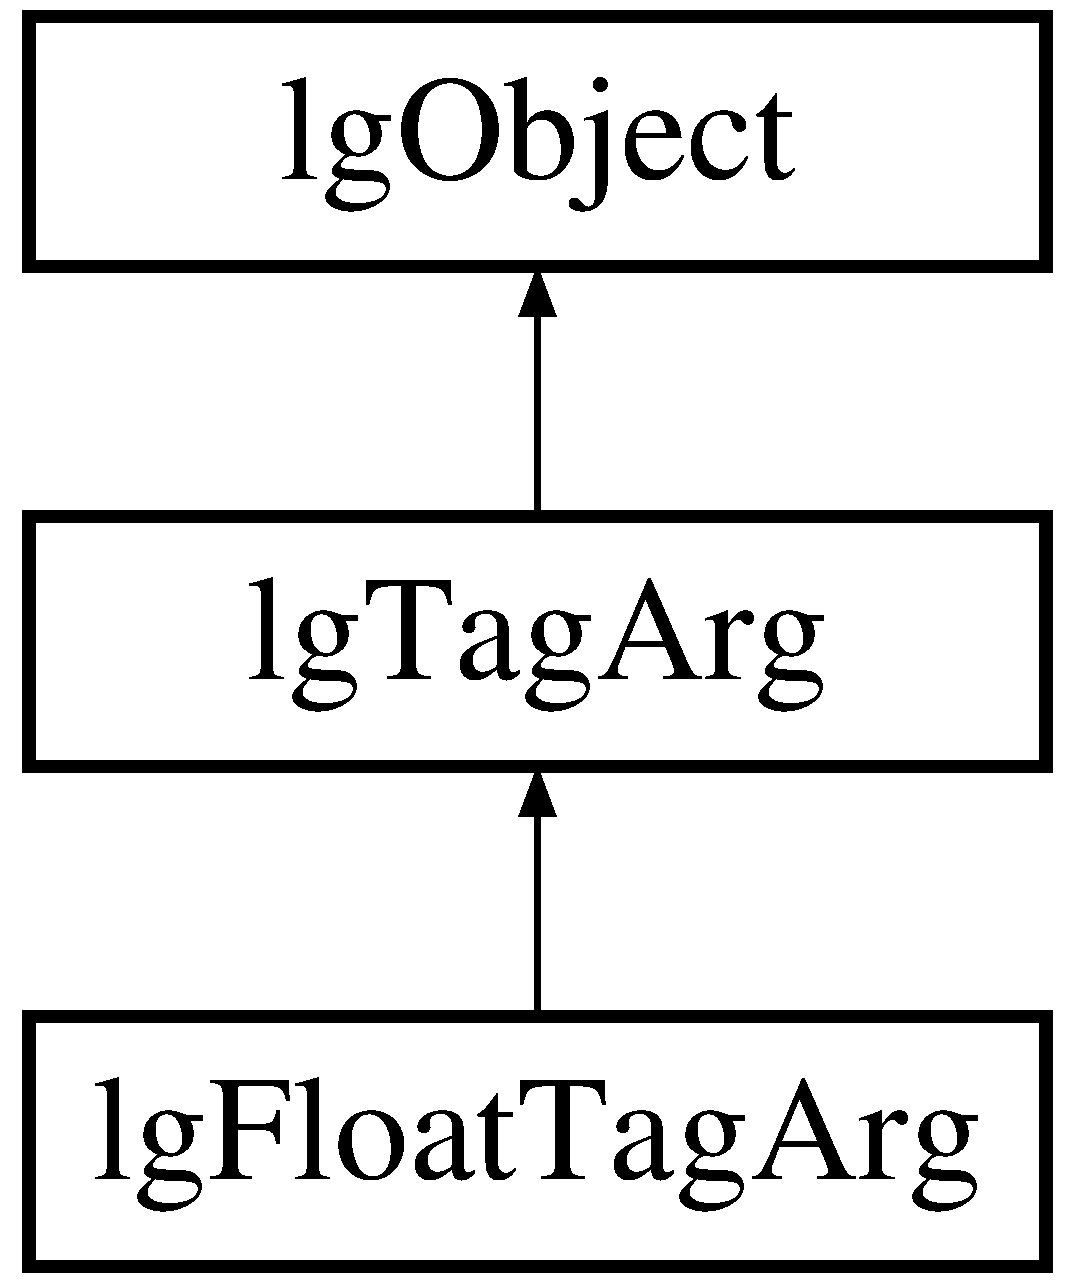
\includegraphics[height=3cm]{classlgFloatTagArg}
\end{center}
\end{figure}
\subsection*{Public Member Functions}
\begin{CompactItemize}
\item 
virtual string {\bf to\-String} ({\bf lg\-Voice} $\ast$seq=NULL)
\item 
{\bf lg\-Float\-Tag\-Arg} (const char $\ast$na, double v, const char $\ast$unit=\char`\"{}\char`\"{})
\item 
virtual double {\bf val\-Float} (void)
\item 
virtual string {\bf val\-Str} (void)
\item 
virtual int {\bf val\-Int} (void)
\item 
virtual void {\bf set\-Val\-Float} (double val)
\end{CompactItemize}
\subsection*{Private Attributes}
\begin{CompactItemize}
\item 
double {\bf val\-I}
\end{CompactItemize}


\subsection{Detailed Description}
double tag argument 



\subsection{Constructor \& Destructor Documentation}
\index{lgFloatTagArg@{lg\-Float\-Tag\-Arg}!lgFloatTagArg@{lgFloatTagArg}}
\index{lgFloatTagArg@{lgFloatTagArg}!lgFloatTagArg@{lg\-Float\-Tag\-Arg}}
\subsubsection{\setlength{\rightskip}{0pt plus 5cm}lg\-Float\-Tag\-Arg::lg\-Float\-Tag\-Arg (const char $\ast$ {\em na}, double {\em v}, const char $\ast$ {\em unit} = \char`\"{}\char`\"{})}\label{classlgFloatTagArg_a1}


\begin{Desc}
\item[Parameters: ]\par
\begin{description}
\item[{\em 
na}]argument name \item[{\em 
v}]argument value \end{description}
\end{Desc}


\subsection{Member Function Documentation}
\index{lgFloatTagArg@{lg\-Float\-Tag\-Arg}!setValFloat@{setValFloat}}
\index{setValFloat@{setValFloat}!lgFloatTagArg@{lg\-Float\-Tag\-Arg}}
\subsubsection{\setlength{\rightskip}{0pt plus 5cm}virtual void lg\-Float\-Tag\-Arg::set\-Val\-Float (double {\em val})\hspace{0.3cm}{\tt  [inline, virtual]}}\label{classlgFloatTagArg_a5}


\index{lgFloatTagArg@{lg\-Float\-Tag\-Arg}!toString@{toString}}
\index{toString@{toString}!lgFloatTagArg@{lg\-Float\-Tag\-Arg}}
\subsubsection{\setlength{\rightskip}{0pt plus 5cm}string lg\-Float\-Tag\-Arg::to\-String ({\bf lg\-Voice} $\ast$ {\em v} = NULL)\hspace{0.3cm}{\tt  [virtual]}}\label{classlgFloatTagArg_a0}


get GUIDO string should be redefined in all derived classes 

Reimplemented from {\bf lg\-Tag\-Arg} {\rm (p.\,\pageref{classlgTagArg_a0})}.\index{lgFloatTagArg@{lg\-Float\-Tag\-Arg}!valFloat@{valFloat}}
\index{valFloat@{valFloat}!lgFloatTagArg@{lg\-Float\-Tag\-Arg}}
\subsubsection{\setlength{\rightskip}{0pt plus 5cm}virtual double lg\-Float\-Tag\-Arg::val\-Float (void)\hspace{0.3cm}{\tt  [inline, virtual]}}\label{classlgFloatTagArg_a2}




Reimplemented from {\bf lg\-Tag\-Arg} {\rm (p.\,\pageref{classlgTagArg_a5})}.\index{lgFloatTagArg@{lg\-Float\-Tag\-Arg}!valInt@{valInt}}
\index{valInt@{valInt}!lgFloatTagArg@{lg\-Float\-Tag\-Arg}}
\subsubsection{\setlength{\rightskip}{0pt plus 5cm}virtual int lg\-Float\-Tag\-Arg::val\-Int (void)\hspace{0.3cm}{\tt  [inline, virtual]}}\label{classlgFloatTagArg_a4}




Reimplemented from {\bf lg\-Tag\-Arg} {\rm (p.\,\pageref{classlgTagArg_a4})}.\index{lgFloatTagArg@{lg\-Float\-Tag\-Arg}!valStr@{valStr}}
\index{valStr@{valStr}!lgFloatTagArg@{lg\-Float\-Tag\-Arg}}
\subsubsection{\setlength{\rightskip}{0pt plus 5cm}virtual string lg\-Float\-Tag\-Arg::val\-Str (void)\hspace{0.3cm}{\tt  [inline, virtual]}}\label{classlgFloatTagArg_a3}




Reimplemented from {\bf lg\-Tag\-Arg} {\rm (p.\,\pageref{classlgTagArg_a3})}.

\subsection{Member Data Documentation}
\index{lgFloatTagArg@{lg\-Float\-Tag\-Arg}!valI@{valI}}
\index{valI@{valI}!lgFloatTagArg@{lg\-Float\-Tag\-Arg}}
\subsubsection{\setlength{\rightskip}{0pt plus 5cm}double {\bf lg\-Float\-Tag\-Arg::val\-I}\hspace{0.3cm}{\tt  [private]}}\label{classlgFloatTagArg_r0}




The documentation for this class was generated from the following files:\begin{CompactItemize}
\item 
{\bf lgtagarg.h}\item 
{\bf lgtagarg.cpp}\end{CompactItemize}

\section{lg\-Int\-Tag\-Arg Class Reference}
\label{classlgIntTagArg}\index{lgIntTagArg@{lgIntTagArg}}
integer tag argument  


{\tt \#include $<$lgtagarg.h$>$}

Inheritance diagram for lg\-Int\-Tag\-Arg::\begin{figure}[H]
\begin{center}
\leavevmode
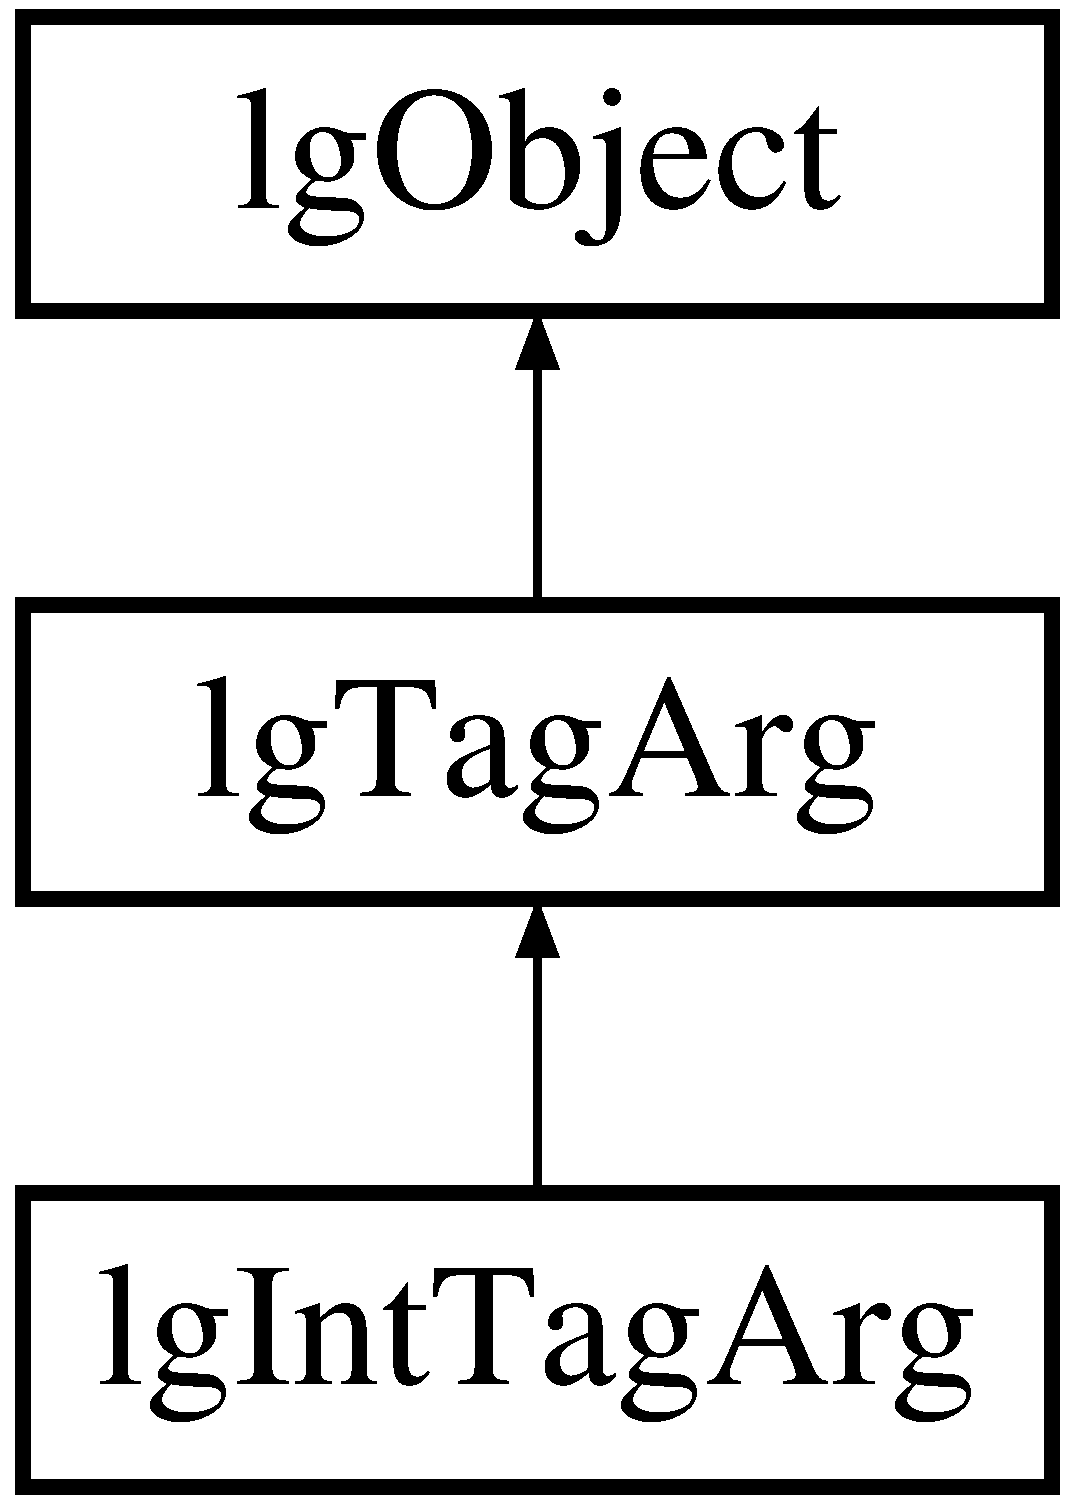
\includegraphics[height=3cm]{classlgIntTagArg}
\end{center}
\end{figure}
\subsection*{Public Member Functions}
\begin{CompactItemize}
\item 
virtual string {\bf to\-String} ({\bf lg\-Voice} $\ast$seq=NULL)
\item 
{\bf lg\-Int\-Tag\-Arg} (const char $\ast$na, int v, const char $\ast$unit=\char`\"{}\char`\"{})
\item 
virtual int {\bf val\-Int} (void)
\item 
virtual double {\bf val\-Float} (void)
\item 
virtual string {\bf val\-Str} (void)
\item 
virtual void {\bf set\-Val\-Int} (int val)
\end{CompactItemize}
\subsection*{Private Attributes}
\begin{CompactItemize}
\item 
int {\bf val\-I}
\end{CompactItemize}


\subsection{Detailed Description}
integer tag argument 



\subsection{Constructor \& Destructor Documentation}
\index{lgIntTagArg@{lg\-Int\-Tag\-Arg}!lgIntTagArg@{lgIntTagArg}}
\index{lgIntTagArg@{lgIntTagArg}!lgIntTagArg@{lg\-Int\-Tag\-Arg}}
\subsubsection{\setlength{\rightskip}{0pt plus 5cm}lg\-Int\-Tag\-Arg::lg\-Int\-Tag\-Arg (const char $\ast$ {\em na}, int {\em v}, const char $\ast$ {\em unit} = \char`\"{}\char`\"{})}\label{classlgIntTagArg_a1}


\begin{Desc}
\item[Parameters: ]\par
\begin{description}
\item[{\em 
na}]argument name, might be \char`\"{}\char`\"{} \item[{\em 
v}]argument value \end{description}
\end{Desc}


\subsection{Member Function Documentation}
\index{lgIntTagArg@{lg\-Int\-Tag\-Arg}!setValInt@{setValInt}}
\index{setValInt@{setValInt}!lgIntTagArg@{lg\-Int\-Tag\-Arg}}
\subsubsection{\setlength{\rightskip}{0pt plus 5cm}virtual void lg\-Int\-Tag\-Arg::set\-Val\-Int (int {\em val})\hspace{0.3cm}{\tt  [inline, virtual]}}\label{classlgIntTagArg_a5}


\index{lgIntTagArg@{lg\-Int\-Tag\-Arg}!toString@{toString}}
\index{toString@{toString}!lgIntTagArg@{lg\-Int\-Tag\-Arg}}
\subsubsection{\setlength{\rightskip}{0pt plus 5cm}string lg\-Int\-Tag\-Arg::to\-String ({\bf lg\-Voice} $\ast$ {\em v} = NULL)\hspace{0.3cm}{\tt  [virtual]}}\label{classlgIntTagArg_a0}


get GUIDO string should be redefined in all derived classes 

Reimplemented from {\bf lg\-Tag\-Arg} {\rm (p.\,\pageref{classlgTagArg_a0})}.\index{lgIntTagArg@{lg\-Int\-Tag\-Arg}!valFloat@{valFloat}}
\index{valFloat@{valFloat}!lgIntTagArg@{lg\-Int\-Tag\-Arg}}
\subsubsection{\setlength{\rightskip}{0pt plus 5cm}virtual double lg\-Int\-Tag\-Arg::val\-Float (void)\hspace{0.3cm}{\tt  [inline, virtual]}}\label{classlgIntTagArg_a3}




Reimplemented from {\bf lg\-Tag\-Arg} {\rm (p.\,\pageref{classlgTagArg_a5})}.\index{lgIntTagArg@{lg\-Int\-Tag\-Arg}!valInt@{valInt}}
\index{valInt@{valInt}!lgIntTagArg@{lg\-Int\-Tag\-Arg}}
\subsubsection{\setlength{\rightskip}{0pt plus 5cm}virtual int lg\-Int\-Tag\-Arg::val\-Int (void)\hspace{0.3cm}{\tt  [inline, virtual]}}\label{classlgIntTagArg_a2}




Reimplemented from {\bf lg\-Tag\-Arg} {\rm (p.\,\pageref{classlgTagArg_a4})}.\index{lgIntTagArg@{lg\-Int\-Tag\-Arg}!valStr@{valStr}}
\index{valStr@{valStr}!lgIntTagArg@{lg\-Int\-Tag\-Arg}}
\subsubsection{\setlength{\rightskip}{0pt plus 5cm}virtual string lg\-Int\-Tag\-Arg::val\-Str (void)\hspace{0.3cm}{\tt  [inline, virtual]}}\label{classlgIntTagArg_a4}




Reimplemented from {\bf lg\-Tag\-Arg} {\rm (p.\,\pageref{classlgTagArg_a3})}.

\subsection{Member Data Documentation}
\index{lgIntTagArg@{lg\-Int\-Tag\-Arg}!valI@{valI}}
\index{valI@{valI}!lgIntTagArg@{lg\-Int\-Tag\-Arg}}
\subsubsection{\setlength{\rightskip}{0pt plus 5cm}int {\bf lg\-Int\-Tag\-Arg::val\-I}\hspace{0.3cm}{\tt  [private]}}\label{classlgIntTagArg_r0}




The documentation for this class was generated from the following files:\begin{CompactItemize}
\item 
{\bf lgtagarg.h}\item 
{\bf lgtagarg.cpp}\end{CompactItemize}

\section{lg\-Note Class Reference}
\label{classlgNote}\index{lgNote@{lgNote}}
A {\bf lg\-Event} with additional pitch info.  


{\tt \#include $<$lgnote.h$>$}

Inheritance diagram for lg\-Note::\begin{figure}[H]
\begin{center}
\leavevmode
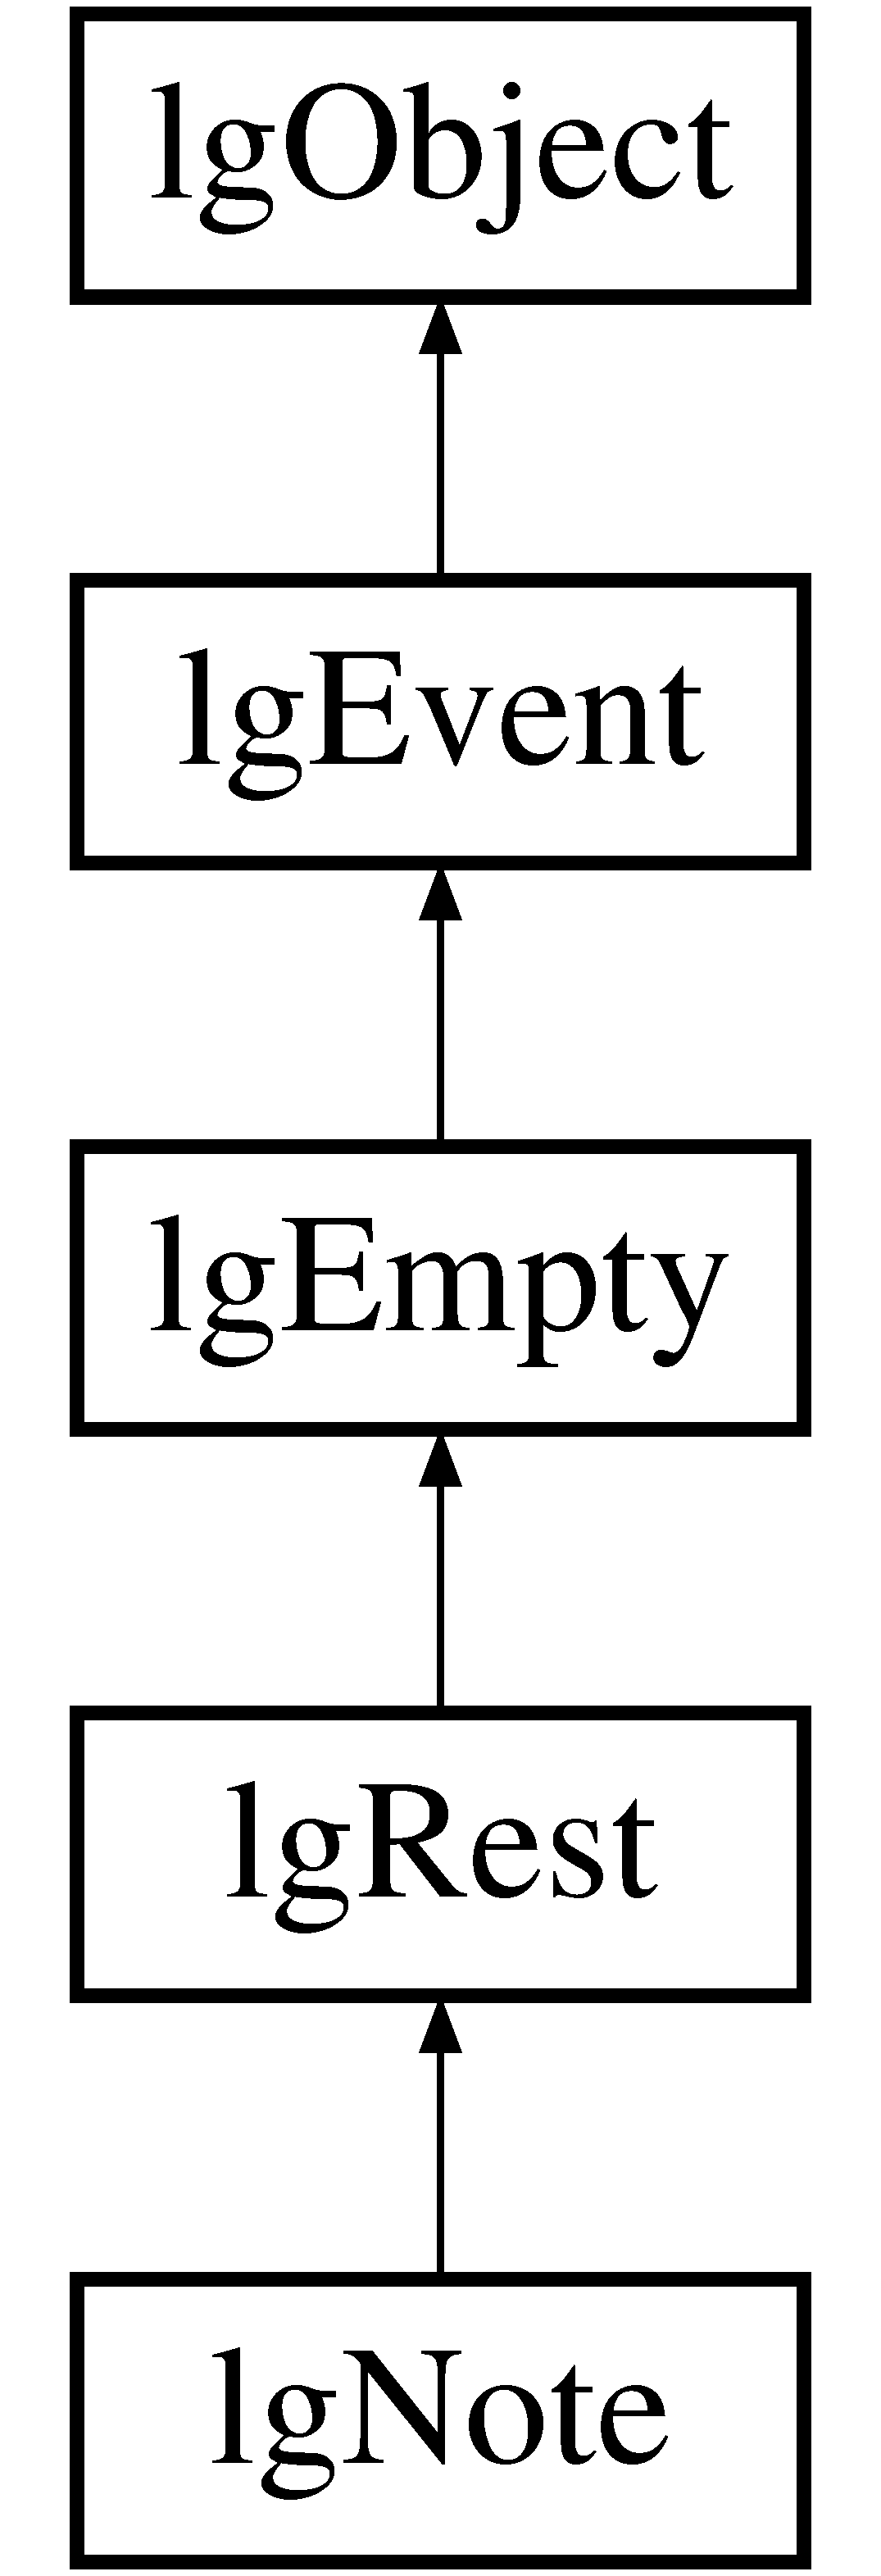
\includegraphics[height=5cm]{classlgNote}
\end{center}
\end{figure}
\subsection*{Public Member Functions}
\begin{CompactItemize}
\item 
virtual string {\bf to\-String} ({\bf lg\-Voice} $\ast$calling\-Seq=NULL)
\begin{CompactList}\small\item\em pitch accidentals octave $\ast$ duration \item\end{CompactList}\item 
int {\bf octave} (void)
\begin{CompactList}\small\item\em -oo...+oo, 0 == c' \item\end{CompactList}\item 
void {\bf set\-Octave} (int i)
\begin{CompactList}\small\item\em -oo...+oo, 0 == c' \item\end{CompactList}\item 
int {\bf pitch\-Class} (void)
\begin{CompactList}\small\item\em 0...11 = c,cis, ... b \item\end{CompactList}\item 
void {\bf set\-Pitch\-Class} (int i)
\begin{CompactList}\small\item\em 0...11 = c,cis, ... b \item\end{CompactList}\item 
int {\bf accidentals} (void)
\begin{CompactList}\small\item\em -oo..+oo \item\end{CompactList}\item 
void {\bf set\-Accidentals} (int i)
\begin{CompactList}\small\item\em -oo..+oo \item\end{CompactList}\item 
{\bf lg\-Note} (int pc, int oct, int acc, long int dur\-Num, long int dur\-Denom, int cdots, long int pos\-Num, long int pos\-Denom)
\item 
string {\bf pitch} (void)
\begin{CompactList}\small\item\em pitch as string \char`\"{}c\char`\"{}, \char`\"{}c\#\char`\"{}, \char`\"{}gis\char`\"{}, \char`\"{}g\#\char`\"{}, ... \item\end{CompactList}\end{CompactItemize}
\subsection*{Private Attributes}
\begin{CompactItemize}
\item 
int {\bf pitch\-Class\-I}
\begin{CompactList}\small\item\em 0..11 = c,cis,...,b \item\end{CompactList}\item 
int {\bf octave\-I}
\begin{CompactList}\small\item\em -oo .. +oo, 0 = c' \item\end{CompactList}\item 
int {\bf accidentals\-I}
\begin{CompactList}\small\item\em -oo .. +oo \item\end{CompactList}\end{CompactItemize}


\subsection{Detailed Description}
A {\bf lg\-Event} with additional pitch info. 



\subsection{Constructor \& Destructor Documentation}
\index{lgNote@{lg\-Note}!lgNote@{lgNote}}
\index{lgNote@{lgNote}!lgNote@{lg\-Note}}
\subsubsection{\setlength{\rightskip}{0pt plus 5cm}lg\-Note::lg\-Note (int {\em pc}, int {\em oct}, int {\em acc}, long int {\em dur\-Num}, long int {\em dur\-Denom}, int {\em cdots}, long int {\em pos\-Num}, long int {\em pos\-Denom})}\label{classlgNote_a7}


\begin{Desc}
\item[Parameters: ]\par
\begin{description}
\item[{\em 
pc}]pitchclass 0..11 \item[{\em 
oct}]octave -oo..+oo, 0 = c' \item[{\em 
acc}]\# of accidentals -oo .. +oo \item[{\em 
dur\-Num}]duration numerator \item[{\em 
dur\-Denom}]duration denominator \item[{\em 
cdots}]\# of dots \item[{\em 
pos\-Num}]position numerator \item[{\em 
pos\-Denom}]position denominator \end{description}
\end{Desc}


\subsection{Member Function Documentation}
\index{lgNote@{lg\-Note}!accidentals@{accidentals}}
\index{accidentals@{accidentals}!lgNote@{lg\-Note}}
\subsubsection{\setlength{\rightskip}{0pt plus 5cm}int lg\-Note::accidentals (void)\hspace{0.3cm}{\tt  [inline]}}\label{classlgNote_a5}


-oo..+oo 

\index{lgNote@{lg\-Note}!octave@{octave}}
\index{octave@{octave}!lgNote@{lg\-Note}}
\subsubsection{\setlength{\rightskip}{0pt plus 5cm}int lg\-Note::octave (void)}\label{classlgNote_a1}


-oo...+oo, 0 == c' 

\index{lgNote@{lg\-Note}!pitch@{pitch}}
\index{pitch@{pitch}!lgNote@{lg\-Note}}
\subsubsection{\setlength{\rightskip}{0pt plus 5cm}string lg\-Note::pitch (void)}\label{classlgNote_a8}


pitch as string \char`\"{}c\char`\"{}, \char`\"{}c\#\char`\"{}, \char`\"{}gis\char`\"{}, \char`\"{}g\#\char`\"{}, ... 

copy pitch class \index{lgNote@{lg\-Note}!pitchClass@{pitchClass}}
\index{pitchClass@{pitchClass}!lgNote@{lg\-Note}}
\subsubsection{\setlength{\rightskip}{0pt plus 5cm}int lg\-Note::pitch\-Class (void)}\label{classlgNote_a3}


0...11 = c,cis, ... b 

\index{lgNote@{lg\-Note}!setAccidentals@{setAccidentals}}
\index{setAccidentals@{setAccidentals}!lgNote@{lg\-Note}}
\subsubsection{\setlength{\rightskip}{0pt plus 5cm}void lg\-Note::set\-Accidentals (int {\em i})\hspace{0.3cm}{\tt  [inline]}}\label{classlgNote_a6}


-oo..+oo 

\index{lgNote@{lg\-Note}!setOctave@{setOctave}}
\index{setOctave@{setOctave}!lgNote@{lg\-Note}}
\subsubsection{\setlength{\rightskip}{0pt plus 5cm}void lg\-Note::set\-Octave (int {\em i})\hspace{0.3cm}{\tt  [inline]}}\label{classlgNote_a2}


-oo...+oo, 0 == c' 

\index{lgNote@{lg\-Note}!setPitchClass@{setPitchClass}}
\index{setPitchClass@{setPitchClass}!lgNote@{lg\-Note}}
\subsubsection{\setlength{\rightskip}{0pt plus 5cm}void lg\-Note::set\-Pitch\-Class (int {\em i})\hspace{0.3cm}{\tt  [inline]}}\label{classlgNote_a4}


0...11 = c,cis, ... b 

\index{lgNote@{lg\-Note}!toString@{toString}}
\index{toString@{toString}!lgNote@{lg\-Note}}
\subsubsection{\setlength{\rightskip}{0pt plus 5cm}string lg\-Note::to\-String ({\bf lg\-Voice} $\ast$ {\em calling\-Seq} = NULL)\hspace{0.3cm}{\tt  [virtual]}}\label{classlgNote_a0}


pitch accidentals octave $\ast$ duration 



Reimplemented from {\bf lg\-Rest} {\rm (p.\,\pageref{classlgRest_a0})}.

\subsection{Member Data Documentation}
\index{lgNote@{lg\-Note}!accidentalsI@{accidentalsI}}
\index{accidentalsI@{accidentalsI}!lgNote@{lg\-Note}}
\subsubsection{\setlength{\rightskip}{0pt plus 5cm}int {\bf lg\-Note::accidentals\-I}\hspace{0.3cm}{\tt  [private]}}\label{classlgNote_r2}


-oo .. +oo 

\index{lgNote@{lg\-Note}!octaveI@{octaveI}}
\index{octaveI@{octaveI}!lgNote@{lg\-Note}}
\subsubsection{\setlength{\rightskip}{0pt plus 5cm}int {\bf lg\-Note::octave\-I}\hspace{0.3cm}{\tt  [private]}}\label{classlgNote_r1}


-oo .. +oo, 0 = c' 

\index{lgNote@{lg\-Note}!pitchClassI@{pitchClassI}}
\index{pitchClassI@{pitchClassI}!lgNote@{lg\-Note}}
\subsubsection{\setlength{\rightskip}{0pt plus 5cm}int {\bf lg\-Note::pitch\-Class\-I}\hspace{0.3cm}{\tt  [private]}}\label{classlgNote_r0}


0..11 = c,cis,...,b 



The documentation for this class was generated from the following files:\begin{CompactItemize}
\item 
{\bf lgnote.h}\item 
{\bf lgnote.cpp}\end{CompactItemize}

\section{lg\-Object Class Reference}
\label{classlgObject}\index{lgObject@{lgObject}}
a GUIDO object with no additional specific info  


{\tt \#include $<$lgobject.h$>$}

Inheritance diagram for lg\-Object::\begin{figure}[H]
\begin{center}
\leavevmode
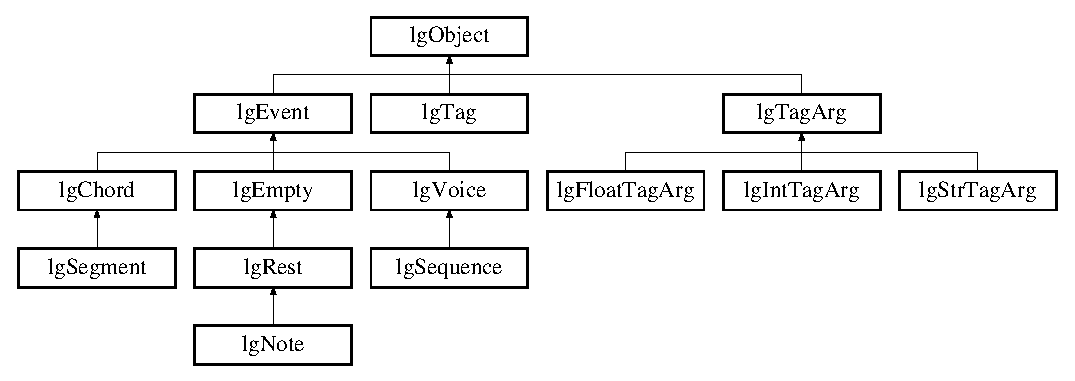
\includegraphics[height=4.66667cm]{classlgObject}
\end{center}
\end{figure}
\subsection*{Public Member Functions}
\begin{CompactItemize}
\item 
void {\bf accept} ({\bf string\-Visitor} v)
\item 
{\bf lg\-Object} $\ast$ {\bf next} (void)
\item 
{\bf lg\-Object} (void)
\item 
virtual string {\bf to\-String} ({\bf lg\-Voice} $\ast$calling\-Seq=NULL)
\item 
virtual void {\bf write} (FILE $\ast$out, {\bf lg\-Voice} $\ast$=NULL)
\begin{CompactList}\small\item\em write in GUIDO Syntax \item\end{CompactList}\item 
virtual {\bf lg\-Duration} {\bf pos} (void)
\end{CompactItemize}
\subsection*{Protected Member Functions}
\begin{CompactItemize}
\item 
virtual void {\bf set\-Next} ({\bf lg\-Object} $\ast$ptr)
\end{CompactItemize}
\subsection*{Protected Attributes}
\begin{CompactItemize}
\item 
{\bf lg\-Object} $\ast$ {\bf next\-I}
\end{CompactItemize}
\subsection*{Friends}
\begin{CompactItemize}
\item 
class {\bf lg\-Event}
\item 
class {\bf lg\-Voice}
\item 
class {\bf lg\-Sequence}
\item 
class {\bf lg\-Segment}
\item 
class {\bf lg\-Tag}
\item 
class {\bf lg\-Chord}
\end{CompactItemize}


\subsection{Detailed Description}
a GUIDO object with no additional specific info 



\subsection{Constructor \& Destructor Documentation}
\index{lgObject@{lg\-Object}!lgObject@{lgObject}}
\index{lgObject@{lgObject}!lgObject@{lg\-Object}}
\subsubsection{\setlength{\rightskip}{0pt plus 5cm}lg\-Object::lg\-Object (void)}\label{classlgObject_a2}




\subsection{Member Function Documentation}
\index{lgObject@{lg\-Object}!accept@{accept}}
\index{accept@{accept}!lgObject@{lg\-Object}}
\subsubsection{\setlength{\rightskip}{0pt plus 5cm}void lg\-Object::accept ({\bf string\-Visitor} {\em v})}\label{classlgObject_a0}




Reimplemented in {\bf lg\-Tag} {\rm (p.\,\pageref{classlgTag_a4})}.\index{lgObject@{lg\-Object}!next@{next}}
\index{next@{next}!lgObject@{lg\-Object}}
\subsubsection{\setlength{\rightskip}{0pt plus 5cm}{\bf lg\-Object}$\ast$ lg\-Object::next (void)\hspace{0.3cm}{\tt  [inline]}}\label{classlgObject_a1}


\index{lgObject@{lg\-Object}!pos@{pos}}
\index{pos@{pos}!lgObject@{lg\-Object}}
\subsubsection{\setlength{\rightskip}{0pt plus 5cm}virtual {\bf lg\-Duration} lg\-Object::pos (void)\hspace{0.3cm}{\tt  [inline, virtual]}}\label{classlgObject_a5}




Reimplemented in {\bf lg\-Event} {\rm (p.\,\pageref{classlgEvent_a6})}, and {\bf lg\-Tag} {\rm (p.\,\pageref{classlgTag_a25})}.\index{lgObject@{lg\-Object}!setNext@{setNext}}
\index{setNext@{setNext}!lgObject@{lg\-Object}}
\subsubsection{\setlength{\rightskip}{0pt plus 5cm}void lg\-Object::set\-Next ({\bf lg\-Object} $\ast$ {\em ptr})\hspace{0.3cm}{\tt  [protected, virtual]}}\label{classlgObject_b0}


\index{lgObject@{lg\-Object}!toString@{toString}}
\index{toString@{toString}!lgObject@{lg\-Object}}
\subsubsection{\setlength{\rightskip}{0pt plus 5cm}virtual string lg\-Object::to\-String ({\bf lg\-Voice} $\ast$ {\em calling\-Seq} = NULL)\hspace{0.3cm}{\tt  [inline, virtual]}}\label{classlgObject_a3}


get GUIDO string should be redefined in all derived classes 

Reimplemented in {\bf lg\-Chord} {\rm (p.\,\pageref{classlgChord_a6})}, {\bf lg\-Empty} {\rm (p.\,\pageref{classlgEmpty_a0})}, {\bf lg\-Event} {\rm (p.\,\pageref{classlgEvent_a1})}, {\bf lg\-Note} {\rm (p.\,\pageref{classlgNote_a0})}, {\bf lg\-Rest} {\rm (p.\,\pageref{classlgRest_a0})}, {\bf lg\-Segment} {\rm (p.\,\pageref{classlgSegment_a21})}, {\bf lg\-Sequence} {\rm (p.\,\pageref{classlgSequence_a0})}, {\bf lg\-Tag} {\rm (p.\,\pageref{classlgTag_a5})}, {\bf lg\-Tag\-Arg} {\rm (p.\,\pageref{classlgTagArg_a0})}, {\bf lg\-Str\-Tag\-Arg} {\rm (p.\,\pageref{classlgStrTagArg_a0})}, {\bf lg\-Int\-Tag\-Arg} {\rm (p.\,\pageref{classlgIntTagArg_a0})}, {\bf lg\-Float\-Tag\-Arg} {\rm (p.\,\pageref{classlgFloatTagArg_a0})}, and {\bf lg\-Voice} {\rm (p.\,\pageref{classlgVoice_a20})}.\index{lgObject@{lg\-Object}!write@{write}}
\index{write@{write}!lgObject@{lg\-Object}}
\subsubsection{\setlength{\rightskip}{0pt plus 5cm}virtual void lg\-Object::write (FILE $\ast$ {\em out}, {\bf lg\-Voice} $\ast$ = NULL)\hspace{0.3cm}{\tt  [inline, virtual]}}\label{classlgObject_a4}


write in GUIDO Syntax 



Reimplemented in {\bf lg\-Chord} {\rm (p.\,\pageref{classlgChord_a7})}, {\bf lg\-Event} {\rm (p.\,\pageref{classlgEvent_a8})}, {\bf lg\-Segment} {\rm (p.\,\pageref{classlgSegment_a22})}, and {\bf lg\-Voice} {\rm (p.\,\pageref{classlgVoice_a21})}.

\subsection{Friends And Related Function Documentation}
\index{lgObject@{lg\-Object}!lgChord@{lgChord}}
\index{lgChord@{lgChord}!lgObject@{lg\-Object}}
\subsubsection{\setlength{\rightskip}{0pt plus 5cm}friend class {\bf lg\-Chord}\hspace{0.3cm}{\tt  [friend]}}\label{classlgObject_n5}




Reimplemented in {\bf lg\-Event} {\rm (p.\,\pageref{classlgEvent_n1})}, {\bf lg\-Tag} {\rm (p.\,\pageref{classlgTag_n0})}, and {\bf lg\-Voice} {\rm (p.\,\pageref{classlgVoice_n0})}.\index{lgObject@{lg\-Object}!lgEvent@{lgEvent}}
\index{lgEvent@{lgEvent}!lgObject@{lg\-Object}}
\subsubsection{\setlength{\rightskip}{0pt plus 5cm}friend class {\bf lg\-Event}\hspace{0.3cm}{\tt  [friend]}}\label{classlgObject_n0}


\index{lgObject@{lg\-Object}!lgSegment@{lgSegment}}
\index{lgSegment@{lgSegment}!lgObject@{lg\-Object}}
\subsubsection{\setlength{\rightskip}{0pt plus 5cm}friend class {\bf lg\-Segment}\hspace{0.3cm}{\tt  [friend]}}\label{classlgObject_n3}




Reimplemented in {\bf lg\-Voice} {\rm (p.\,\pageref{classlgVoice_n1})}.\index{lgObject@{lg\-Object}!lgSequence@{lgSequence}}
\index{lgSequence@{lgSequence}!lgObject@{lg\-Object}}
\subsubsection{\setlength{\rightskip}{0pt plus 5cm}friend class {\bf lg\-Sequence}\hspace{0.3cm}{\tt  [friend]}}\label{classlgObject_n2}


\index{lgObject@{lg\-Object}!lgTag@{lgTag}}
\index{lgTag@{lgTag}!lgObject@{lg\-Object}}
\subsubsection{\setlength{\rightskip}{0pt plus 5cm}friend class {\bf lg\-Tag}\hspace{0.3cm}{\tt  [friend]}}\label{classlgObject_n4}


\index{lgObject@{lg\-Object}!lgVoice@{lgVoice}}
\index{lgVoice@{lgVoice}!lgObject@{lg\-Object}}
\subsubsection{\setlength{\rightskip}{0pt plus 5cm}friend class {\bf lg\-Voice}\hspace{0.3cm}{\tt  [friend]}}\label{classlgObject_n1}




Reimplemented in {\bf lg\-Event} {\rm (p.\,\pageref{classlgEvent_n0})}, and {\bf lg\-Tag} {\rm (p.\,\pageref{classlgTag_n1})}.

\subsection{Member Data Documentation}
\index{lgObject@{lg\-Object}!nextI@{nextI}}
\index{nextI@{nextI}!lgObject@{lg\-Object}}
\subsubsection{\setlength{\rightskip}{0pt plus 5cm}{\bf lg\-Object}$\ast$ {\bf lg\-Object::next\-I}\hspace{0.3cm}{\tt  [protected]}}\label{classlgObject_p0}




The documentation for this class was generated from the following files:\begin{CompactItemize}
\item 
{\bf lgobject.h}\item 
{\bf lgobject.cpp}\end{CompactItemize}

\section{lg\-Rest Class Reference}
\label{classlgRest}\index{lgRest@{lgRest}}
a GUIDO rest based on {\bf lg\-Empty} with Duration  


{\tt \#include $<$lgrest.h$>$}

Inheritance diagram for lg\-Rest::\begin{figure}[H]
\begin{center}
\leavevmode
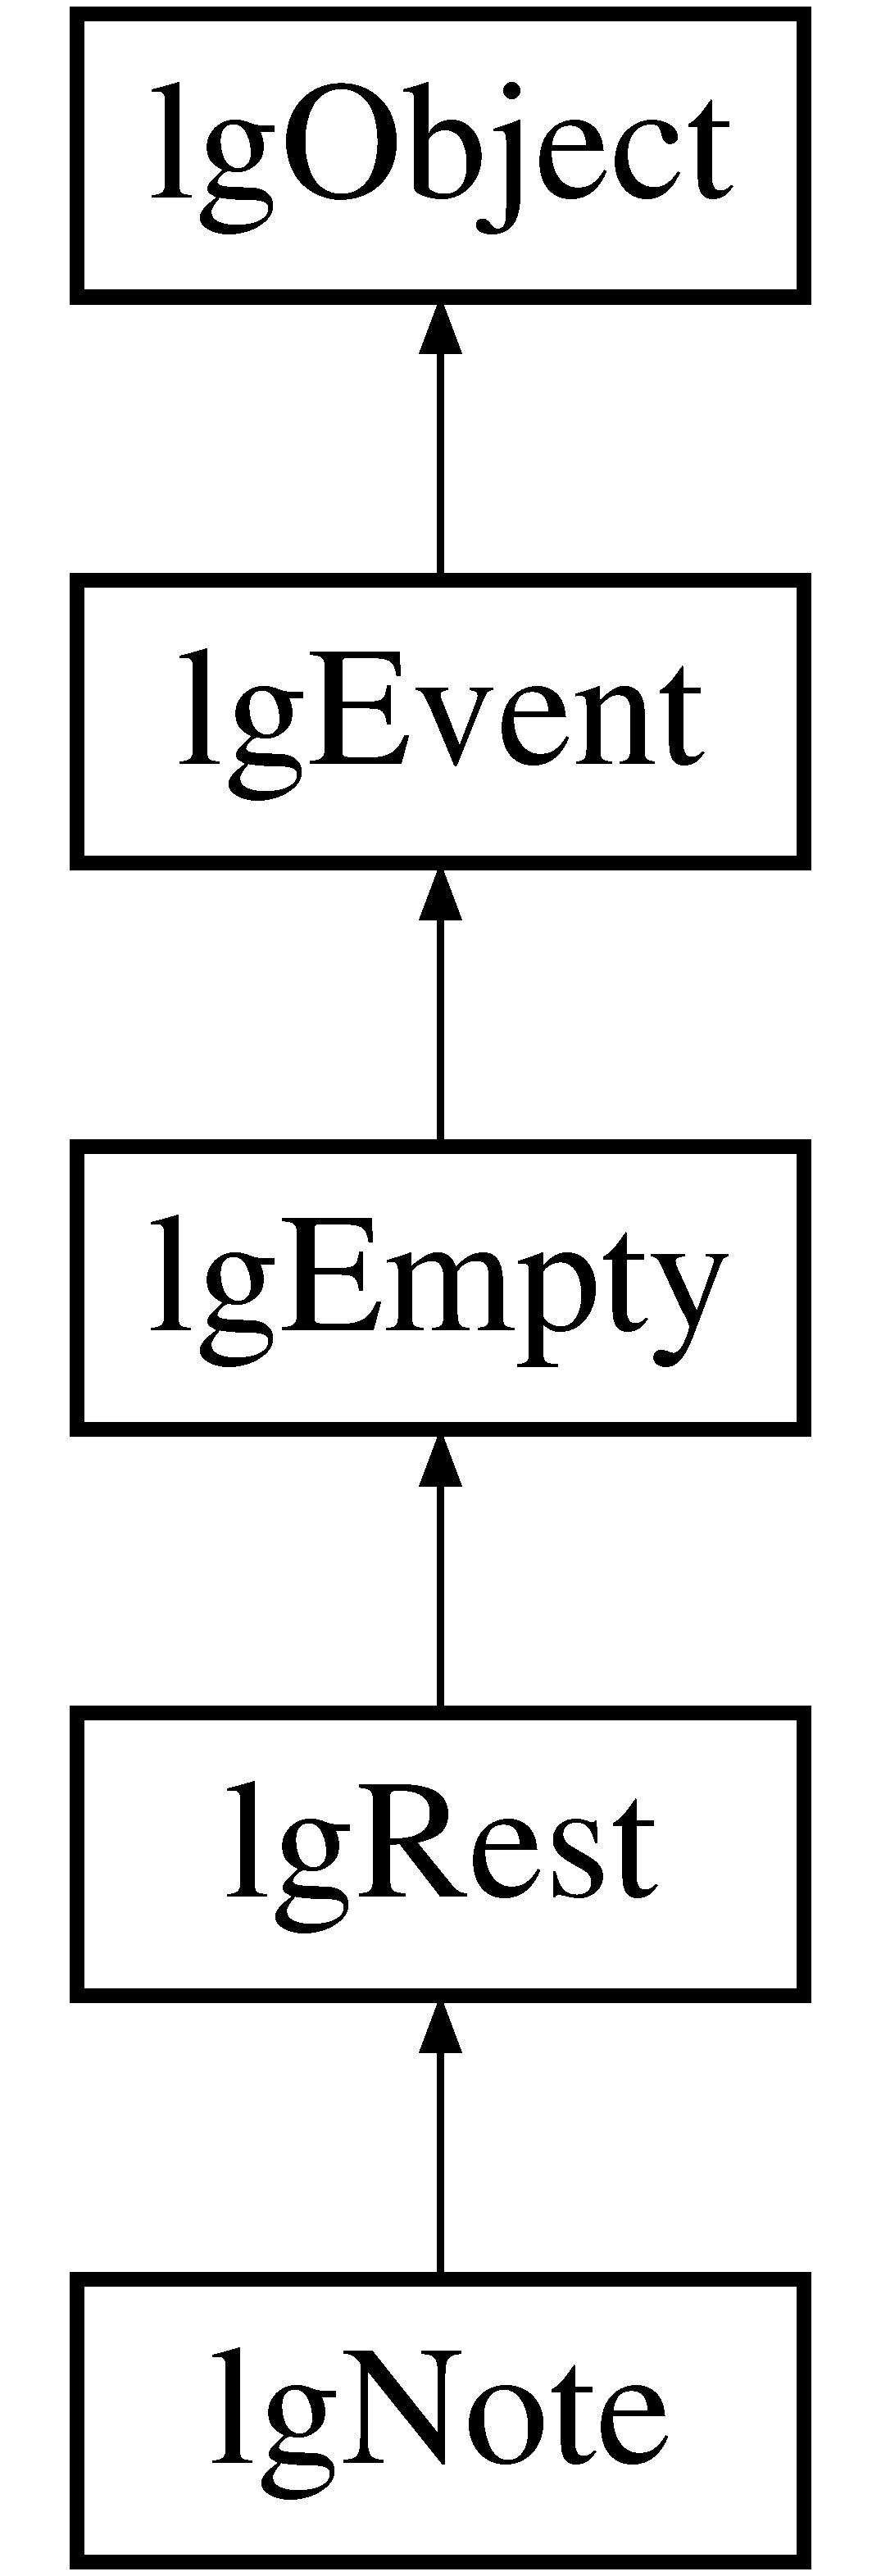
\includegraphics[height=5cm]{classlgRest}
\end{center}
\end{figure}
\subsection*{Public Member Functions}
\begin{CompactItemize}
\item 
virtual string {\bf to\-String} ({\bf lg\-Voice} $\ast$calling\-Seq=NULL)
\begin{CompactList}\small\item\em write \char`\"{}\_\-$\ast$\char`\"{}Duration \item\end{CompactList}\item 
{\bf lg\-Rest} (long int dur\-Nnum, long int dur\-Denom, int cdots, long int pos\-Num, long int pos\-Denom)
\end{CompactItemize}


\subsection{Detailed Description}
a GUIDO rest based on {\bf lg\-Empty} with Duration 



\subsection{Constructor \& Destructor Documentation}
\index{lgRest@{lg\-Rest}!lgRest@{lgRest}}
\index{lgRest@{lgRest}!lgRest@{lg\-Rest}}
\subsubsection{\setlength{\rightskip}{0pt plus 5cm}lg\-Rest::lg\-Rest (long int {\em dur\-Nnum}, long int {\em dur\-Denom}, int {\em cdots}, long int {\em pos\-Num}, long int {\em pos\-Denom})}\label{classlgRest_a1}




\subsection{Member Function Documentation}
\index{lgRest@{lg\-Rest}!toString@{toString}}
\index{toString@{toString}!lgRest@{lg\-Rest}}
\subsubsection{\setlength{\rightskip}{0pt plus 5cm}string lg\-Rest::to\-String ({\bf lg\-Voice} $\ast$ {\em calling\-Seq} = NULL)\hspace{0.3cm}{\tt  [virtual]}}\label{classlgRest_a0}


write \char`\"{}\_\-$\ast$\char`\"{}Duration 



Reimplemented from {\bf lg\-Empty} {\rm (p.\,\pageref{classlgEmpty_a0})}.

Reimplemented in {\bf lg\-Note} {\rm (p.\,\pageref{classlgNote_a0})}.

The documentation for this class was generated from the following files:\begin{CompactItemize}
\item 
{\bf lgrest.h}\item 
{\bf lgrest.cpp}\end{CompactItemize}

\section{lg\-Segment Class Reference}
\label{classlgSegment}\index{lgSegment@{lgSegment}}
GUIDO Segment based on {\bf lg\-Chord} with parsing support.  


{\tt \#include $<$lgsegment.h$>$}

Inheritance diagram for lg\-Segment::\begin{figure}[H]
\begin{center}
\leavevmode
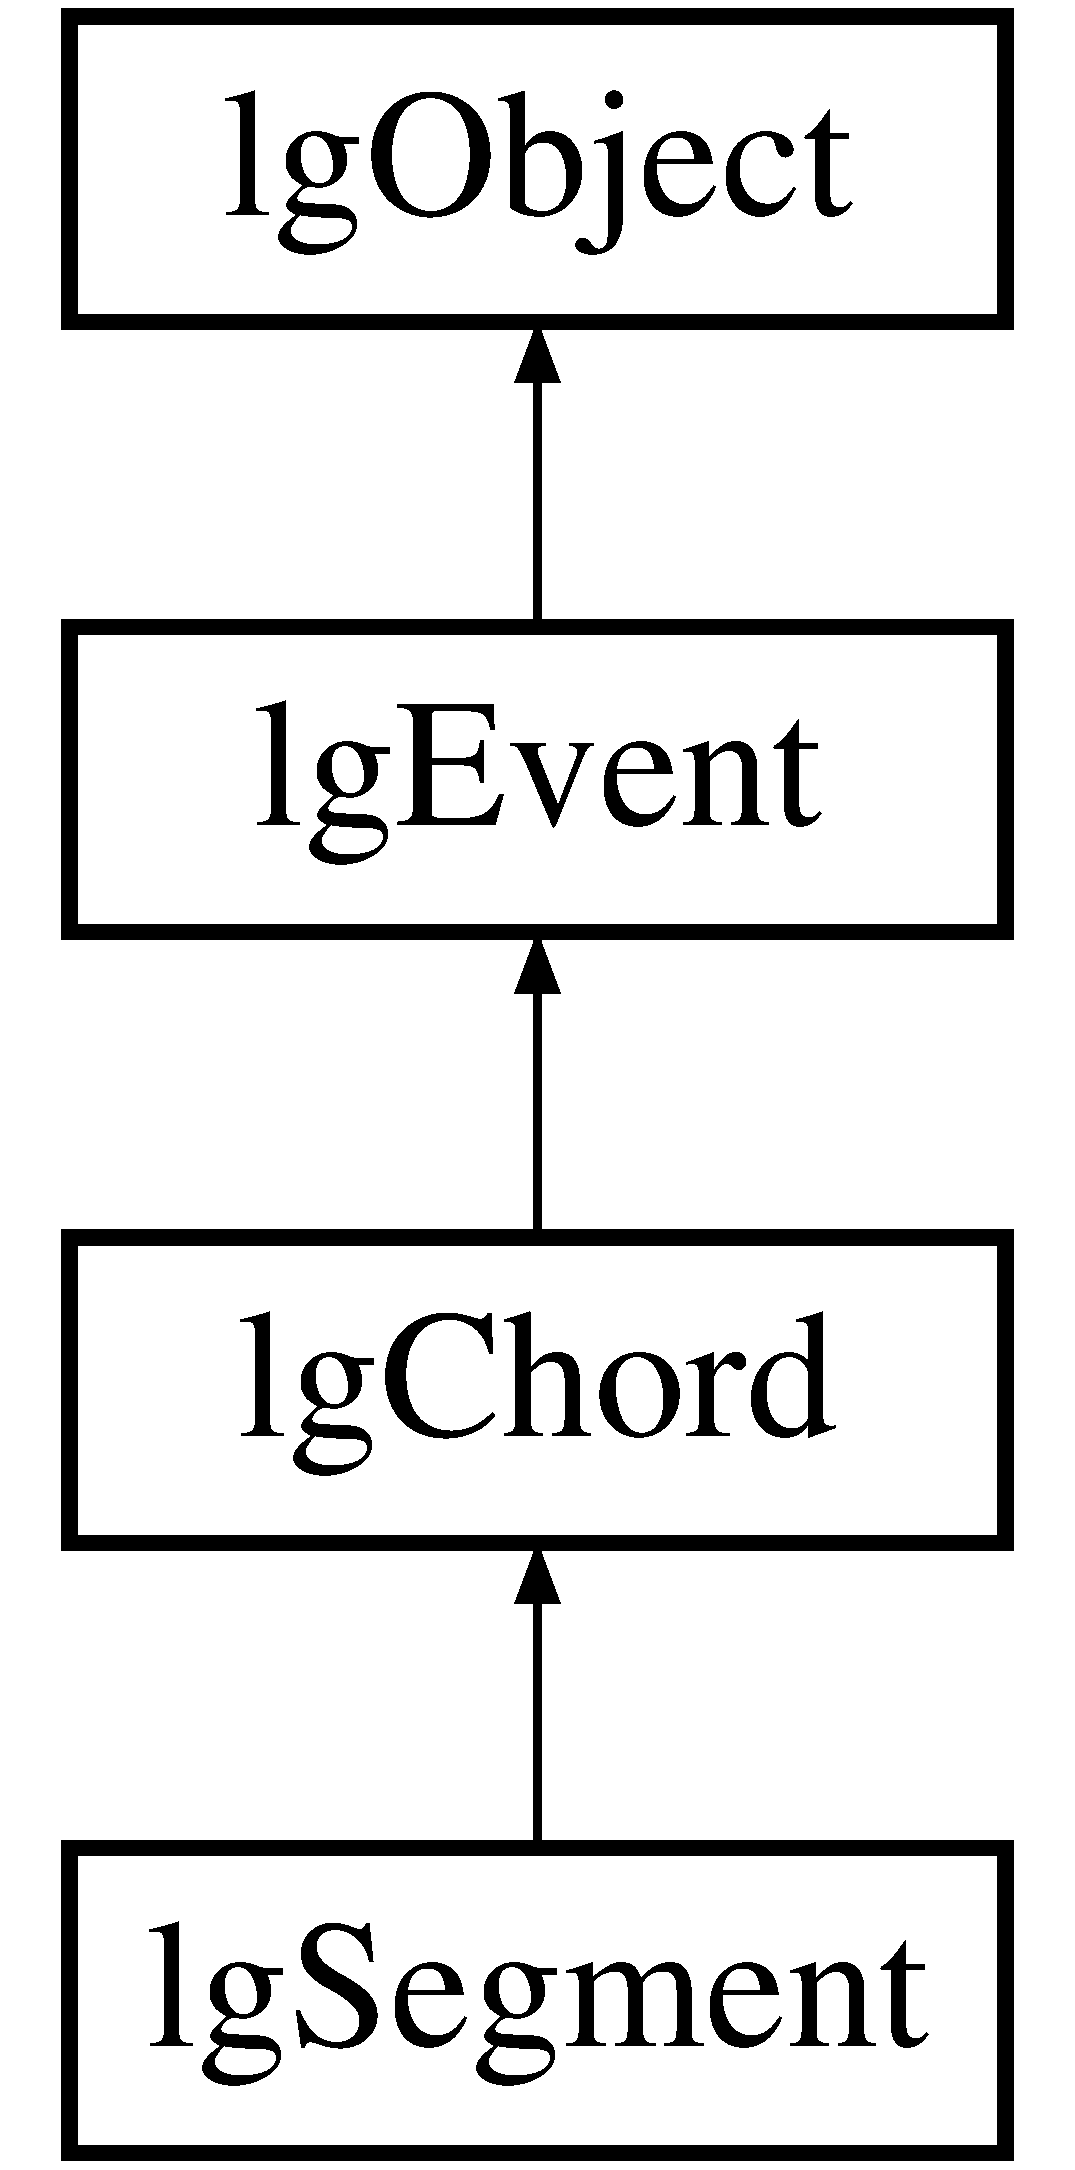
\includegraphics[height=4cm]{classlgSegment}
\end{center}
\end{figure}
\subsection*{Public Member Functions}
\begin{CompactItemize}
\item 
{\bf lg\-Segment} ({\bf lg\-Factory} $\ast$fy)
\item 
int {\bf parse\-GMNFile} (FILE $\ast$file)
\begin{CompactList}\small\item\em result: 0 == ok, 1 == parse error \item\end{CompactList}\item 
int {\bf parse\-GMNFile} (const char $\ast$filename)
\begin{CompactList}\small\item\em result: 0 == ok, 1 == parse error \item\end{CompactList}\item 
int {\bf parse\-String} (char $\ast$str)
\begin{CompactList}\small\item\em result: 0 == ok, 1 == parse error \item\end{CompactList}\item 
int {\bf parse\-String} (string str)
\begin{CompactList}\small\item\em result: 0 == ok, 1 == parse error \item\end{CompactList}\item 
virtual {\bf $\sim$lg\-Segment} (void)
\item 
virtual void {\bf append\-Event} ({\bf lg\-Event} $\ast$ev)
\begin{CompactList}\small\item\em append event in cur\-Sequence OR cur\-Chord!!! \item\end{CompactList}\item 
{\bf lg\-Rest} $\ast$ {\bf append\-Rest} (long int dur\-N, long int dur\-D, int dots, long int dur\-Pos\-N, long int dur\-Pos\-D)
\begin{CompactList}\small\item\em create a new virtual {\bf lg\-Rest} event and append \item\end{CompactList}\item 
void {\bf append\-Empty} (long int dur\-N, long int dur\-D, int dots, long int dur\-Pos\-N, long int dur\-Pos\-D)
\begin{CompactList}\small\item\em create a new virtual {\bf lg\-Empty} and append \item\end{CompactList}\item 
{\bf lg\-Note} $\ast$ {\bf append\-Note} (int pc, int oct, int acc, long int dur\-N, long int dur\-D, int dots, long int dur\-Pos\-N, long int dur\-Pos\-D)
\begin{CompactList}\small\item\em create a new virtual {\bf lg\-Note} and append \item\end{CompactList}\item 
{\bf lg\-Chord} $\ast$ {\bf append\-Chord} ({\bf lg\-Chord} $\ast$ch)
\begin{CompactList}\small\item\em append chord in cur\-Sequence, if ch == NULL -$>$ close current chord, return == appended chord! \item\end{CompactList}\item 
void {\bf insert\-Tag} ({\bf lg\-Tag} $\ast${\bf tag})
\begin{CompactList}\small\item\em append tag in cur\-Sequence \item\end{CompactList}\item 
virtual {\bf lg\-Tag} $\ast$ {\bf append\-Tag} (long int {\bf tagno}, const char $\ast$tagname)
\begin{CompactList}\small\item\em append a tag to cur\-Sequence-$>$[cur\-Chord\-Voice] \item\end{CompactList}\item 
{\bf lg\-Chord} $\ast$ {\bf init\-Chord} (long int pos\-Num, long int pos\-Denom)
\begin{CompactList}\small\item\em create a new chord in cur\-Sequence \item\end{CompactList}\item 
void {\bf init\-Chord\-Voice} (void)
\begin{CompactList}\small\item\em create a new voice in cur\-Chord \item\end{CompactList}\item 
void {\bf exit\-Chord\-Voice} (void)
\begin{CompactList}\small\item\em close cur\-Voice \item\end{CompactList}\item 
virtual {\bf lg\-Sequence} $\ast$ {\bf append\-Sequence} ({\bf lg\-Sequence} $\ast$seq=NULL)
\begin{CompactList}\small\item\em append a new sequence and store in cur\-Sequence, if seq == NULL a sequence will be created \item\end{CompactList}\item 
void {\bf exit\-Sequence} (void)
\begin{CompactList}\small\item\em leave, close the current sequence if parsing a ']' \item\end{CompactList}\item 
void {\bf close\-Tag} (long int id)
\item 
{\bf lg\-Sequence} $\ast$ {\bf first\-Sequence} (void)
\item 
{\bf lg\-Sequence} $\ast$ {\bf next\-Sequence} (void)
\item 
virtual string {\bf to\-String} ({\bf lg\-Voice} $\ast$calling\-Seq=NULL)
\begin{CompactList}\small\item\em reset the close\-Range stack for events/tags of all voices \item\end{CompactList}\item 
virtual void {\bf write} (FILE $\ast$out, {\bf lg\-Voice} $\ast$v=NULL)
\begin{CompactList}\small\item\em write own data AND all tags starting in call\-Seq in (this-$>$pos...next-$>$pos] \item\end{CompactList}\item 
virtual void {\bf write\-File} (const char $\ast$fname)
\item 
{\bf lg\-Sequence} $\ast$ {\bf search\-By\-ID} (int n)
\end{CompactItemize}
\subsection*{Public Attributes}
\begin{CompactItemize}
\item 
{\bf lg\-Factory} $\ast$ {\bf factory}
\begin{CompactList}\small\item\em ptr to the factory object \item\end{CompactList}\end{CompactItemize}
\subsection*{Private Attributes}
\begin{CompactItemize}
\item 
{\bf lg\-Sequence} $\ast$ {\bf cur\-Sequence}
\begin{CompactList}\small\item\em cur\-Pointers for parsing \item\end{CompactList}\item 
{\bf lg\-Chord} $\ast$ {\bf cur\-Chord}
\item 
{\bf lg\-Event} $\ast$ {\bf cur\-Event}
\item 
{\bf lg\-Tag} $\ast$ {\bf cur\-Tag}
\item 
{\bf lg\-Voice} $\ast$ {\bf cur\-Chord\-Voice}
\end{CompactItemize}


\subsection{Detailed Description}
GUIDO Segment based on {\bf lg\-Chord} with parsing support. 



\subsection{Constructor \& Destructor Documentation}
\index{lgSegment@{lg\-Segment}!lgSegment@{lgSegment}}
\index{lgSegment@{lgSegment}!lgSegment@{lg\-Segment}}
\subsubsection{\setlength{\rightskip}{0pt plus 5cm}lg\-Segment::lg\-Segment ({\bf lg\-Factory} $\ast$ {\em fy})}\label{classlgSegment_a0}


\index{lgSegment@{lg\-Segment}!~lgSegment@{$\sim$lgSegment}}
\index{~lgSegment@{$\sim$lgSegment}!lgSegment@{lg\-Segment}}
\subsubsection{\setlength{\rightskip}{0pt plus 5cm}lg\-Segment::$\sim${\bf lg\-Segment} (void)\hspace{0.3cm}{\tt  [virtual]}}\label{classlgSegment_a5}




\subsection{Member Function Documentation}
\index{lgSegment@{lg\-Segment}!appendChord@{appendChord}}
\index{appendChord@{appendChord}!lgSegment@{lg\-Segment}}
\subsubsection{\setlength{\rightskip}{0pt plus 5cm}{\bf lg\-Chord} $\ast$ lg\-Segment::append\-Chord ({\bf lg\-Chord} $\ast$ {\em ch})}\label{classlgSegment_a10}


append chord in cur\-Sequence, if ch == NULL -$>$ close current chord, return == appended chord! 

\index{lgSegment@{lg\-Segment}!appendEmpty@{appendEmpty}}
\index{appendEmpty@{appendEmpty}!lgSegment@{lg\-Segment}}
\subsubsection{\setlength{\rightskip}{0pt plus 5cm}void lg\-Segment::append\-Empty (long int {\em dur\-N}, long int {\em dur\-D}, int {\em dots}, long int {\em dur\-Pos\-N}, long int {\em dur\-Pos\-D})\hspace{0.3cm}{\tt  [inline]}}\label{classlgSegment_a8}


create a new virtual {\bf lg\-Empty} and append 

\index{lgSegment@{lg\-Segment}!appendEvent@{appendEvent}}
\index{appendEvent@{appendEvent}!lgSegment@{lg\-Segment}}
\subsubsection{\setlength{\rightskip}{0pt plus 5cm}void lg\-Segment::append\-Event ({\bf lg\-Event} $\ast$ {\em ev})\hspace{0.3cm}{\tt  [virtual]}}\label{classlgSegment_a6}


append event in cur\-Sequence OR cur\-Chord!!! 

we are inside a chord

create new voice in chord! 

Reimplemented from {\bf lg\-Chord} {\rm (p.\,\pageref{classlgChord_a3})}.\index{lgSegment@{lg\-Segment}!appendNote@{appendNote}}
\index{appendNote@{appendNote}!lgSegment@{lg\-Segment}}
\subsubsection{\setlength{\rightskip}{0pt plus 5cm}{\bf lg\-Note}$\ast$ lg\-Segment::append\-Note (int {\em pc}, int {\em oct}, int {\em acc}, long int {\em dur\-N}, long int {\em dur\-D}, int {\em dots}, long int {\em dur\-Pos\-N}, long int {\em dur\-Pos\-D})\hspace{0.3cm}{\tt  [inline]}}\label{classlgSegment_a9}


create a new virtual {\bf lg\-Note} and append 

\index{lgSegment@{lg\-Segment}!appendRest@{appendRest}}
\index{appendRest@{appendRest}!lgSegment@{lg\-Segment}}
\subsubsection{\setlength{\rightskip}{0pt plus 5cm}{\bf lg\-Rest}$\ast$ lg\-Segment::append\-Rest (long int {\em dur\-N}, long int {\em dur\-D}, int {\em dots}, long int {\em dur\-Pos\-N}, long int {\em dur\-Pos\-D})\hspace{0.3cm}{\tt  [inline]}}\label{classlgSegment_a7}


create a new virtual {\bf lg\-Rest} event and append 

\index{lgSegment@{lg\-Segment}!appendSequence@{appendSequence}}
\index{appendSequence@{appendSequence}!lgSegment@{lg\-Segment}}
\subsubsection{\setlength{\rightskip}{0pt plus 5cm}{\bf lg\-Sequence} $\ast$ lg\-Segment::append\-Sequence ({\bf lg\-Sequence} $\ast$ {\em seq} = NULL)\hspace{0.3cm}{\tt  [virtual]}}\label{classlgSegment_a16}


append a new sequence and store in cur\-Sequence, if seq == NULL a sequence will be created 

\index{lgSegment@{lg\-Segment}!appendTag@{appendTag}}
\index{appendTag@{appendTag}!lgSegment@{lg\-Segment}}
\subsubsection{\setlength{\rightskip}{0pt plus 5cm}{\bf lg\-Tag} $\ast$ lg\-Segment::append\-Tag (long int {\em tagno}, const char $\ast$ {\em tagname})\hspace{0.3cm}{\tt  [virtual]}}\label{classlgSegment_a12}


append a tag to cur\-Sequence-$>$[cur\-Chord\-Voice] 

create a new tag and append overwrite this function for tag semantics check! \index{lgSegment@{lg\-Segment}!closeTag@{closeTag}}
\index{closeTag@{closeTag}!lgSegment@{lg\-Segment}}
\subsubsection{\setlength{\rightskip}{0pt plus 5cm}void lg\-Segment::close\-Tag (long int {\em id})}\label{classlgSegment_a18}


\index{lgSegment@{lg\-Segment}!exitChordVoice@{exitChordVoice}}
\index{exitChordVoice@{exitChordVoice}!lgSegment@{lg\-Segment}}
\subsubsection{\setlength{\rightskip}{0pt plus 5cm}void lg\-Segment::exit\-Chord\-Voice (void)}\label{classlgSegment_a15}


close cur\-Voice 

\index{lgSegment@{lg\-Segment}!exitSequence@{exitSequence}}
\index{exitSequence@{exitSequence}!lgSegment@{lg\-Segment}}
\subsubsection{\setlength{\rightskip}{0pt plus 5cm}void lg\-Segment::exit\-Sequence (void)}\label{classlgSegment_a17}


leave, close the current sequence if parsing a ']' 

\index{lgSegment@{lg\-Segment}!firstSequence@{firstSequence}}
\index{firstSequence@{firstSequence}!lgSegment@{lg\-Segment}}
\subsubsection{\setlength{\rightskip}{0pt plus 5cm}{\bf lg\-Sequence}$\ast$ lg\-Segment::first\-Sequence (void)\hspace{0.3cm}{\tt  [inline]}}\label{classlgSegment_a19}


\index{lgSegment@{lg\-Segment}!initChord@{initChord}}
\index{initChord@{initChord}!lgSegment@{lg\-Segment}}
\subsubsection{\setlength{\rightskip}{0pt plus 5cm}{\bf lg\-Chord} $\ast$ lg\-Segment::init\-Chord (long int {\em pos\-Num}, long int {\em pos\-Denom})}\label{classlgSegment_a13}


create a new chord in cur\-Sequence 

\index{lgSegment@{lg\-Segment}!initChordVoice@{initChordVoice}}
\index{initChordVoice@{initChordVoice}!lgSegment@{lg\-Segment}}
\subsubsection{\setlength{\rightskip}{0pt plus 5cm}void lg\-Segment::init\-Chord\-Voice (void)}\label{classlgSegment_a14}


create a new voice in cur\-Chord 

\index{lgSegment@{lg\-Segment}!insertTag@{insertTag}}
\index{insertTag@{insertTag}!lgSegment@{lg\-Segment}}
\subsubsection{\setlength{\rightskip}{0pt plus 5cm}void lg\-Segment::insert\-Tag ({\bf lg\-Tag} $\ast$ {\em tag})}\label{classlgSegment_a11}


append tag in cur\-Sequence 

tag might be NULLL if it should be ignored! \index{lgSegment@{lg\-Segment}!nextSequence@{nextSequence}}
\index{nextSequence@{nextSequence}!lgSegment@{lg\-Segment}}
\subsubsection{\setlength{\rightskip}{0pt plus 5cm}{\bf lg\-Sequence}$\ast$ lg\-Segment::next\-Sequence (void)\hspace{0.3cm}{\tt  [inline]}}\label{classlgSegment_a20}


\index{lgSegment@{lg\-Segment}!parseGMNFile@{parseGMNFile}}
\index{parseGMNFile@{parseGMNFile}!lgSegment@{lg\-Segment}}
\subsubsection{\setlength{\rightskip}{0pt plus 5cm}int lg\-Segment::parse\-GMNFile (const char $\ast$ {\em filename})}\label{classlgSegment_a2}


result: 0 == ok, 1 == parse error 

parse a .gmn file and fille the data structure result: 0 = ok 1 = error

pointers for parsing \index{lgSegment@{lg\-Segment}!parseGMNFile@{parseGMNFile}}
\index{parseGMNFile@{parseGMNFile}!lgSegment@{lg\-Segment}}
\subsubsection{\setlength{\rightskip}{0pt plus 5cm}int lg\-Segment::parse\-GMNFile (FILE $\ast$ {\em file})}\label{classlgSegment_a1}


result: 0 == ok, 1 == parse error 

\index{lgSegment@{lg\-Segment}!parseString@{parseString}}
\index{parseString@{parseString}!lgSegment@{lg\-Segment}}
\subsubsection{\setlength{\rightskip}{0pt plus 5cm}int lg\-Segment::parse\-String (string {\em str})\hspace{0.3cm}{\tt  [inline]}}\label{classlgSegment_a4}


result: 0 == ok, 1 == parse error 

\index{lgSegment@{lg\-Segment}!parseString@{parseString}}
\index{parseString@{parseString}!lgSegment@{lg\-Segment}}
\subsubsection{\setlength{\rightskip}{0pt plus 5cm}int lg\-Segment::parse\-String (char $\ast$ {\em str})}\label{classlgSegment_a3}


result: 0 == ok, 1 == parse error 

\index{lgSegment@{lg\-Segment}!searchByID@{searchByID}}
\index{searchByID@{searchByID}!lgSegment@{lg\-Segment}}
\subsubsection{\setlength{\rightskip}{0pt plus 5cm}{\bf lg\-Sequence}$\ast$ lg\-Segment::search\-By\-ID (int {\em n})\hspace{0.3cm}{\tt  [inline]}}\label{classlgSegment_a24}


\index{lgSegment@{lg\-Segment}!toString@{toString}}
\index{toString@{toString}!lgSegment@{lg\-Segment}}
\subsubsection{\setlength{\rightskip}{0pt plus 5cm}virtual string lg\-Segment::to\-String ({\bf lg\-Voice} $\ast$ {\em calling\-Seq} = NULL)\hspace{0.3cm}{\tt  [inline, virtual]}}\label{classlgSegment_a21}


reset the close\-Range stack for events/tags of all voices 

write all tags between this and next call\-Seq might be NULL for Segements 

Reimplemented from {\bf lg\-Chord} {\rm (p.\,\pageref{classlgChord_a6})}.\index{lgSegment@{lg\-Segment}!write@{write}}
\index{write@{write}!lgSegment@{lg\-Segment}}
\subsubsection{\setlength{\rightskip}{0pt plus 5cm}virtual void lg\-Segment::write (FILE $\ast$ {\em out}, {\bf lg\-Voice} $\ast$ {\em v} = NULL)\hspace{0.3cm}{\tt  [inline, virtual]}}\label{classlgSegment_a22}


write own data AND all tags starting in call\-Seq in (this-$>$pos...next-$>$pos] 



Reimplemented from {\bf lg\-Chord} {\rm (p.\,\pageref{classlgChord_a7})}.\index{lgSegment@{lg\-Segment}!writeFile@{writeFile}}
\index{writeFile@{writeFile}!lgSegment@{lg\-Segment}}
\subsubsection{\setlength{\rightskip}{0pt plus 5cm}virtual void lg\-Segment::write\-File (const char $\ast$ {\em fname})\hspace{0.3cm}{\tt  [inline, virtual]}}\label{classlgSegment_a23}




\subsection{Member Data Documentation}
\index{lgSegment@{lg\-Segment}!curChord@{curChord}}
\index{curChord@{curChord}!lgSegment@{lg\-Segment}}
\subsubsection{\setlength{\rightskip}{0pt plus 5cm}{\bf lg\-Chord}$\ast$ {\bf lg\-Segment::cur\-Chord}\hspace{0.3cm}{\tt  [private]}}\label{classlgSegment_r1}


\index{lgSegment@{lg\-Segment}!curChordVoice@{curChordVoice}}
\index{curChordVoice@{curChordVoice}!lgSegment@{lg\-Segment}}
\subsubsection{\setlength{\rightskip}{0pt plus 5cm}{\bf lg\-Voice}$\ast$ {\bf lg\-Segment::cur\-Chord\-Voice}\hspace{0.3cm}{\tt  [private]}}\label{classlgSegment_r4}


\index{lgSegment@{lg\-Segment}!curEvent@{curEvent}}
\index{curEvent@{curEvent}!lgSegment@{lg\-Segment}}
\subsubsection{\setlength{\rightskip}{0pt plus 5cm}{\bf lg\-Event}$\ast$ {\bf lg\-Segment::cur\-Event}\hspace{0.3cm}{\tt  [private]}}\label{classlgSegment_r2}


\index{lgSegment@{lg\-Segment}!curSequence@{curSequence}}
\index{curSequence@{curSequence}!lgSegment@{lg\-Segment}}
\subsubsection{\setlength{\rightskip}{0pt plus 5cm}{\bf lg\-Sequence}$\ast$ {\bf lg\-Segment::cur\-Sequence}\hspace{0.3cm}{\tt  [private]}}\label{classlgSegment_r0}


cur\-Pointers for parsing 

\index{lgSegment@{lg\-Segment}!curTag@{curTag}}
\index{curTag@{curTag}!lgSegment@{lg\-Segment}}
\subsubsection{\setlength{\rightskip}{0pt plus 5cm}{\bf lg\-Tag}$\ast$ {\bf lg\-Segment::cur\-Tag}\hspace{0.3cm}{\tt  [private]}}\label{classlgSegment_r3}


\index{lgSegment@{lg\-Segment}!factory@{factory}}
\index{factory@{factory}!lgSegment@{lg\-Segment}}
\subsubsection{\setlength{\rightskip}{0pt plus 5cm}{\bf lg\-Factory}$\ast$ {\bf lg\-Segment::factory}}\label{classlgSegment_o0}


ptr to the factory object 



The documentation for this class was generated from the following files:\begin{CompactItemize}
\item 
{\bf lgsegment.h}\item 
{\bf lgsegment.cpp}\end{CompactItemize}

\section{lg\-Sequence Class Reference}
\label{classlgSequence}\index{lgSequence@{lgSequence}}
a {\bf lg\-Voice} used as GUIDO Sequence  


{\tt \#include $<$lgsequence.h$>$}

Inheritance diagram for lg\-Sequence::\begin{figure}[H]
\begin{center}
\leavevmode
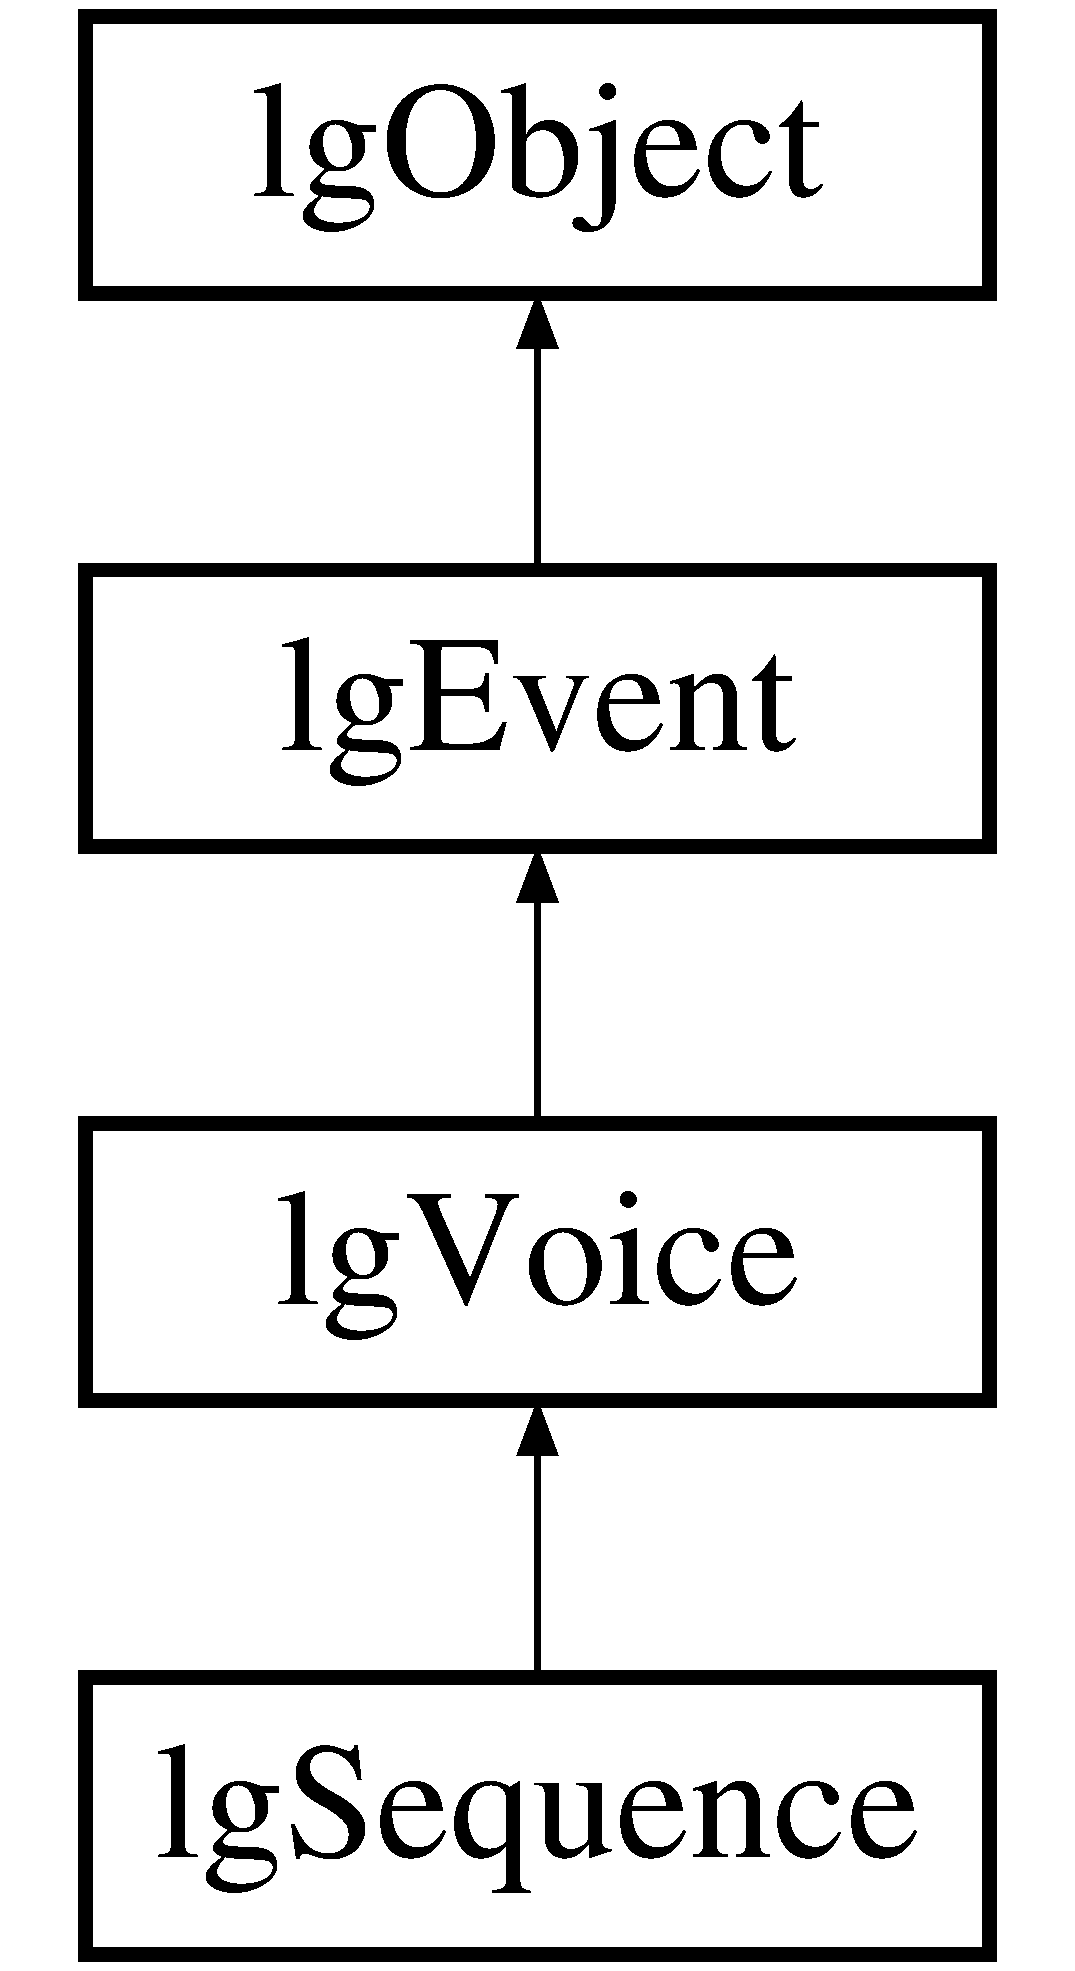
\includegraphics[height=4cm]{classlgSequence}
\end{center}
\end{figure}
\subsection*{Public Member Functions}
\begin{CompactItemize}
\item 
virtual string {\bf to\-String} ({\bf lg\-Voice} $\ast$calling\-Seq=NULL)
\item 
{\bf lg\-Sequence} (long int pos\-Num, long int pos\-Denom)
\item 
void {\bf set\-ID} (int id)
\item 
int {\bf get\-ID} (void)
\end{CompactItemize}
\subsection*{Private Attributes}
\begin{CompactItemize}
\item 
int {\bf ID}
\end{CompactItemize}


\subsection{Detailed Description}
a {\bf lg\-Voice} used as GUIDO Sequence 



\subsection{Constructor \& Destructor Documentation}
\index{lgSequence@{lg\-Sequence}!lgSequence@{lgSequence}}
\index{lgSequence@{lgSequence}!lgSequence@{lg\-Sequence}}
\subsubsection{\setlength{\rightskip}{0pt plus 5cm}lg\-Sequence::lg\-Sequence (long int {\em pos\-Num}, long int {\em pos\-Denom})}\label{classlgSequence_a1}




\subsection{Member Function Documentation}
\index{lgSequence@{lg\-Sequence}!getID@{getID}}
\index{getID@{getID}!lgSequence@{lg\-Sequence}}
\subsubsection{\setlength{\rightskip}{0pt plus 5cm}int lg\-Sequence::get\-ID (void)}\label{classlgSequence_a3}


\index{lgSequence@{lg\-Sequence}!setID@{setID}}
\index{setID@{setID}!lgSequence@{lg\-Sequence}}
\subsubsection{\setlength{\rightskip}{0pt plus 5cm}void lg\-Sequence::set\-ID (int {\em id})}\label{classlgSequence_a2}


\index{lgSequence@{lg\-Sequence}!toString@{toString}}
\index{toString@{toString}!lgSequence@{lg\-Sequence}}
\subsubsection{\setlength{\rightskip}{0pt plus 5cm}string lg\-Sequence::to\-String ({\bf lg\-Voice} $\ast$ {\em calling\-Seq} = NULL)\hspace{0.3cm}{\tt  [virtual]}}\label{classlgSequence_a0}


tags at beginn of the voice 

write event

write all tags after event 

Reimplemented from {\bf lg\-Voice} {\rm (p.\,\pageref{classlgVoice_a20})}.

\subsection{Member Data Documentation}
\index{lgSequence@{lg\-Sequence}!ID@{ID}}
\index{ID@{ID}!lgSequence@{lg\-Sequence}}
\subsubsection{\setlength{\rightskip}{0pt plus 5cm}int {\bf lg\-Sequence::ID}\hspace{0.3cm}{\tt  [private]}}\label{classlgSequence_r0}




The documentation for this class was generated from the following files:\begin{CompactItemize}
\item 
{\bf lgsequence.h}\item 
{\bf lgsequence.cpp}\end{CompactItemize}

\section{lg\-Str\-Tag\-Arg Class Reference}
\label{classlgStrTagArg}\index{lgStrTagArg@{lgStrTagArg}}
string tag argument  


{\tt \#include $<$lgtagarg.h$>$}

Inheritance diagram for lg\-Str\-Tag\-Arg::\begin{figure}[H]
\begin{center}
\leavevmode
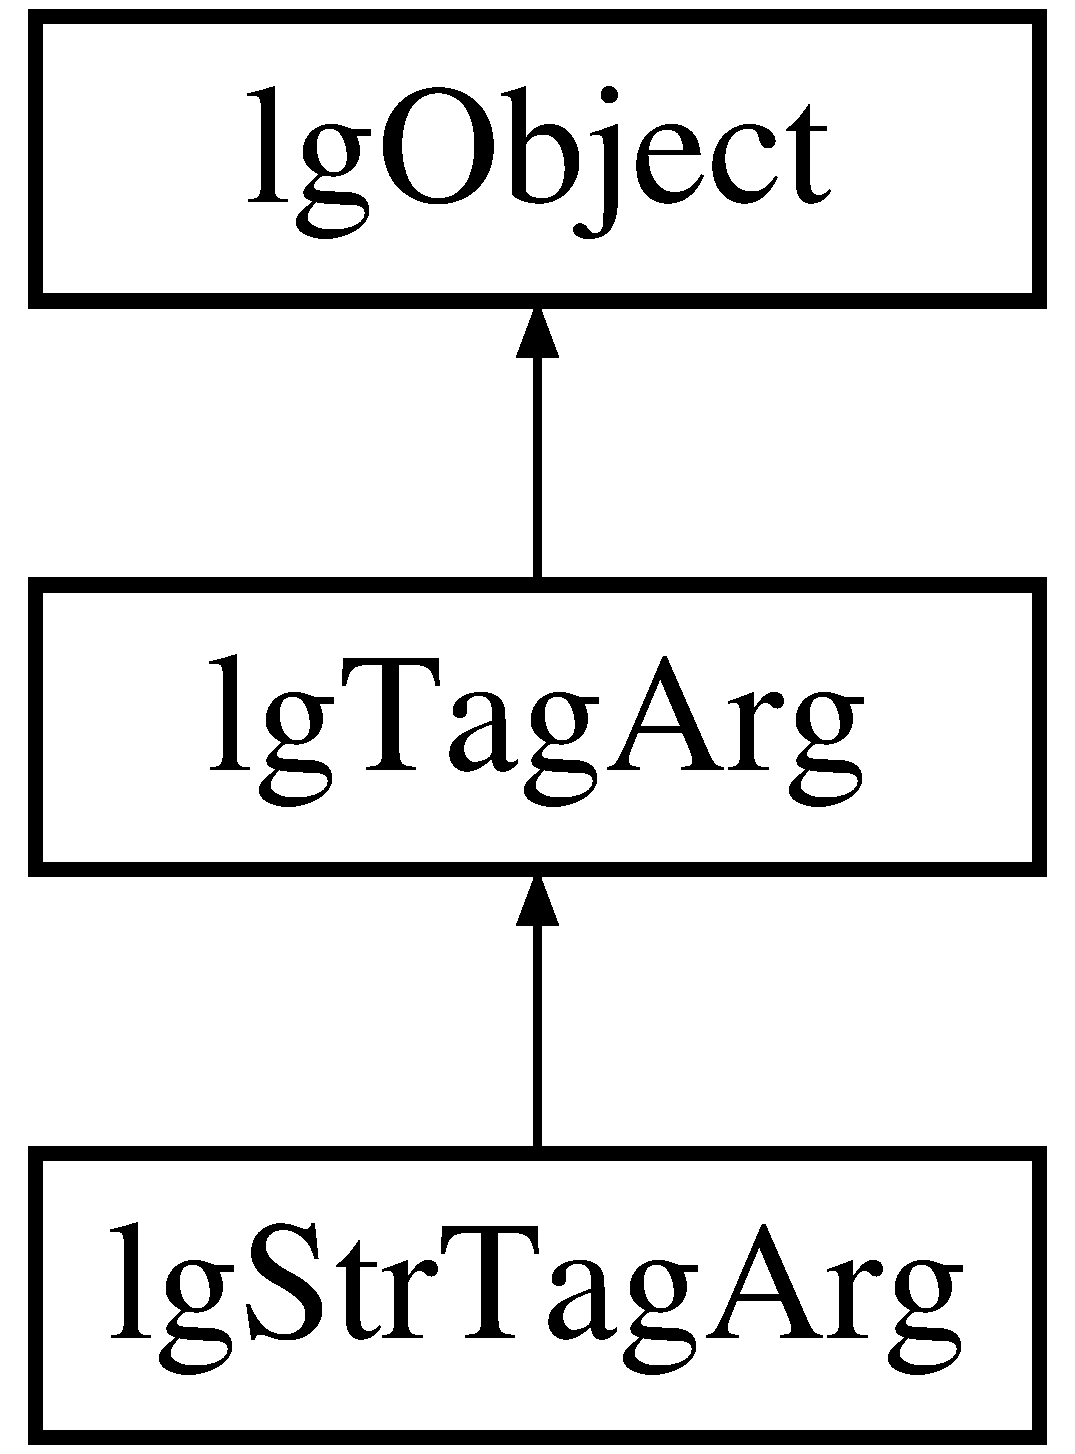
\includegraphics[height=3cm]{classlgStrTagArg}
\end{center}
\end{figure}
\subsection*{Public Member Functions}
\begin{CompactItemize}
\item 
virtual string {\bf to\-String} ({\bf lg\-Voice} $\ast$seq=NULL)
\item 
{\bf lg\-Str\-Tag\-Arg} (const char $\ast$na, const char $\ast$v)
\item 
virtual {\bf $\sim$lg\-Str\-Tag\-Arg} (void)
\item 
virtual string {\bf val\-Str} (void)
\item 
virtual int {\bf val\-Int} (void)
\item 
virtual double {\bf val\-Float} (void)
\item 
virtual void {\bf set\-Val\-Str} (const char $\ast$val)
\end{CompactItemize}
\subsection*{Private Attributes}
\begin{CompactItemize}
\item 
string {\bf val\-I}
\end{CompactItemize}


\subsection{Detailed Description}
string tag argument 



\subsection{Constructor \& Destructor Documentation}
\index{lgStrTagArg@{lg\-Str\-Tag\-Arg}!lgStrTagArg@{lgStrTagArg}}
\index{lgStrTagArg@{lgStrTagArg}!lgStrTagArg@{lg\-Str\-Tag\-Arg}}
\subsubsection{\setlength{\rightskip}{0pt plus 5cm}lg\-Str\-Tag\-Arg::lg\-Str\-Tag\-Arg (const char $\ast$ {\em na}, const char $\ast$ {\em v})}\label{classlgStrTagArg_a1}


\begin{Desc}
\item[Parameters: ]\par
\begin{description}
\item[{\em 
na}]argument name \item[{\em 
v}]argument value \end{description}
\end{Desc}
\index{lgStrTagArg@{lg\-Str\-Tag\-Arg}!~lgStrTagArg@{$\sim$lgStrTagArg}}
\index{~lgStrTagArg@{$\sim$lgStrTagArg}!lgStrTagArg@{lg\-Str\-Tag\-Arg}}
\subsubsection{\setlength{\rightskip}{0pt plus 5cm}lg\-Str\-Tag\-Arg::$\sim${\bf lg\-Str\-Tag\-Arg} (void)\hspace{0.3cm}{\tt  [virtual]}}\label{classlgStrTagArg_a2}




\subsection{Member Function Documentation}
\index{lgStrTagArg@{lg\-Str\-Tag\-Arg}!setValStr@{setValStr}}
\index{setValStr@{setValStr}!lgStrTagArg@{lg\-Str\-Tag\-Arg}}
\subsubsection{\setlength{\rightskip}{0pt plus 5cm}virtual void lg\-Str\-Tag\-Arg::set\-Val\-Str (const char $\ast$ {\em val})\hspace{0.3cm}{\tt  [inline, virtual]}}\label{classlgStrTagArg_a6}


\index{lgStrTagArg@{lg\-Str\-Tag\-Arg}!toString@{toString}}
\index{toString@{toString}!lgStrTagArg@{lg\-Str\-Tag\-Arg}}
\subsubsection{\setlength{\rightskip}{0pt plus 5cm}string lg\-Str\-Tag\-Arg::to\-String ({\bf lg\-Voice} $\ast$ {\em v} = NULL)\hspace{0.3cm}{\tt  [virtual]}}\label{classlgStrTagArg_a0}


get GUIDO string should be redefined in all derived classes 

Reimplemented from {\bf lg\-Tag\-Arg} {\rm (p.\,\pageref{classlgTagArg_a0})}.\index{lgStrTagArg@{lg\-Str\-Tag\-Arg}!valFloat@{valFloat}}
\index{valFloat@{valFloat}!lgStrTagArg@{lg\-Str\-Tag\-Arg}}
\subsubsection{\setlength{\rightskip}{0pt plus 5cm}virtual double lg\-Str\-Tag\-Arg::val\-Float (void)\hspace{0.3cm}{\tt  [inline, virtual]}}\label{classlgStrTagArg_a5}




Reimplemented from {\bf lg\-Tag\-Arg} {\rm (p.\,\pageref{classlgTagArg_a5})}.\index{lgStrTagArg@{lg\-Str\-Tag\-Arg}!valInt@{valInt}}
\index{valInt@{valInt}!lgStrTagArg@{lg\-Str\-Tag\-Arg}}
\subsubsection{\setlength{\rightskip}{0pt plus 5cm}virtual int lg\-Str\-Tag\-Arg::val\-Int (void)\hspace{0.3cm}{\tt  [inline, virtual]}}\label{classlgStrTagArg_a4}




Reimplemented from {\bf lg\-Tag\-Arg} {\rm (p.\,\pageref{classlgTagArg_a4})}.\index{lgStrTagArg@{lg\-Str\-Tag\-Arg}!valStr@{valStr}}
\index{valStr@{valStr}!lgStrTagArg@{lg\-Str\-Tag\-Arg}}
\subsubsection{\setlength{\rightskip}{0pt plus 5cm}virtual string lg\-Str\-Tag\-Arg::val\-Str (void)\hspace{0.3cm}{\tt  [inline, virtual]}}\label{classlgStrTagArg_a3}




Reimplemented from {\bf lg\-Tag\-Arg} {\rm (p.\,\pageref{classlgTagArg_a3})}.

\subsection{Member Data Documentation}
\index{lgStrTagArg@{lg\-Str\-Tag\-Arg}!valI@{valI}}
\index{valI@{valI}!lgStrTagArg@{lg\-Str\-Tag\-Arg}}
\subsubsection{\setlength{\rightskip}{0pt plus 5cm}string {\bf lg\-Str\-Tag\-Arg::val\-I}\hspace{0.3cm}{\tt  [private]}}\label{classlgStrTagArg_r0}




The documentation for this class was generated from the following files:\begin{CompactItemize}
\item 
{\bf lgtagarg.h}\item 
{\bf lgtagarg.cpp}\end{CompactItemize}

\section{lg\-Tag Class Reference}
\label{classlgTag}\index{lgTag@{lgTag}}
GUIDO tag with name and a list of arguments given as {\bf lg\-Tag\-Arg}.  


{\tt \#include $<$lgtag.h$>$}

Inheritance diagram for lg\-Tag::\begin{figure}[H]
\begin{center}
\leavevmode
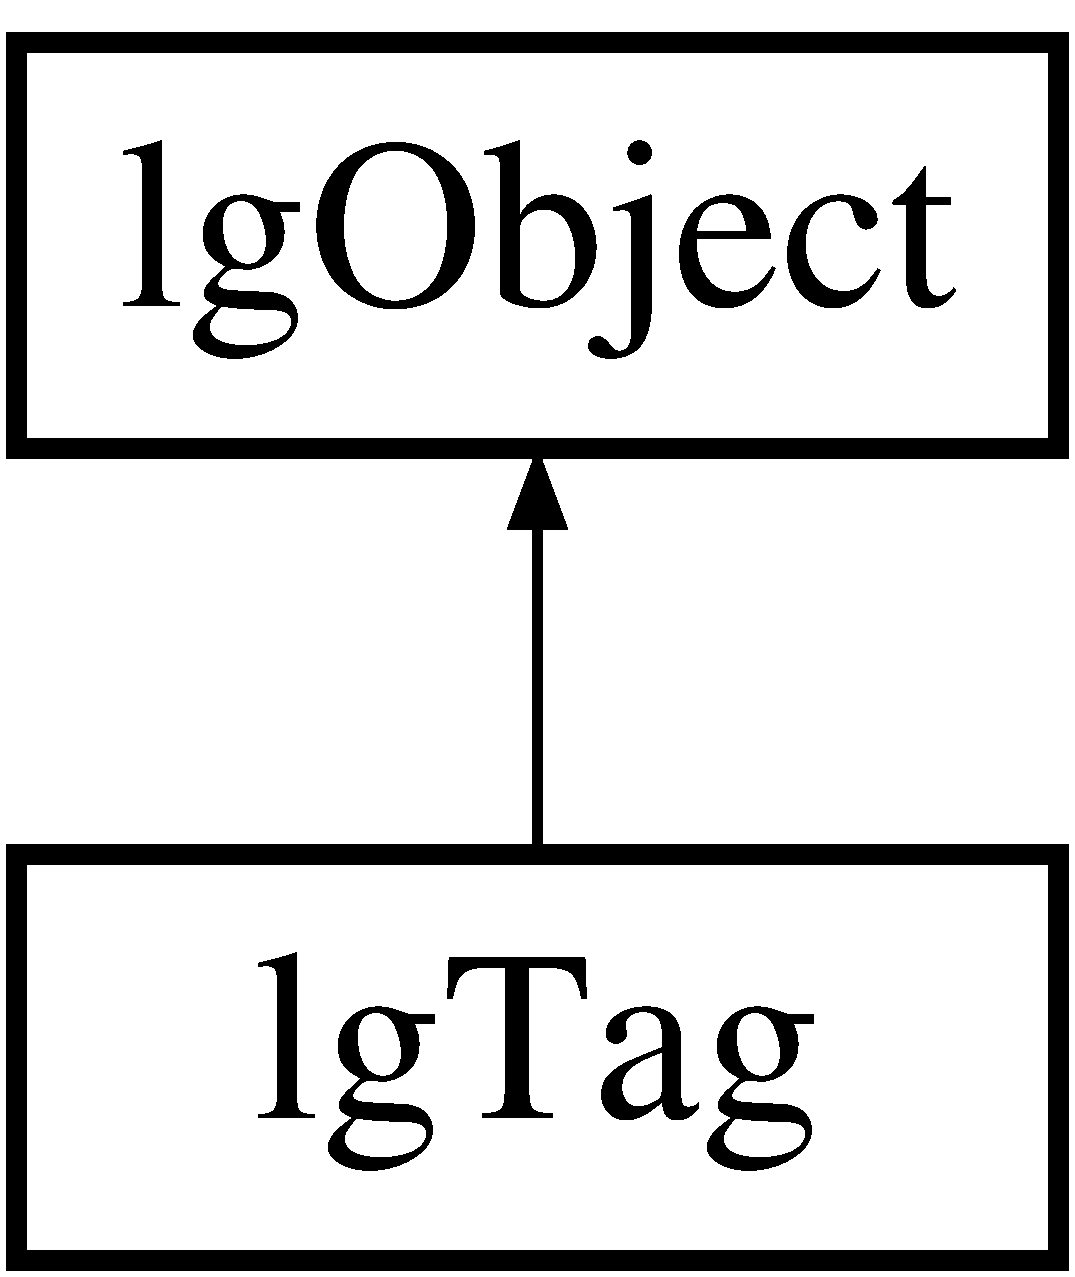
\includegraphics[height=2cm]{classlgTag}
\end{center}
\end{figure}
\subsection*{Public Member Functions}
\begin{CompactItemize}
\item 
int {\bf tag\-Type} (void)
\item 
int {\bf get\-Param\-Char} (const char $\ast$pname, int def\-Pos, string \&value, string \&unit)
\begin{CompactList}\small\item\em get parameter value as a string, return 0 if parameter does not exist \item\end{CompactList}\item 
int {\bf get\-Param\-Int} (const char $\ast$pname, int def\-Pos, int \&value, string \&unit)
\begin{CompactList}\small\item\em get parameter value as an int, return 0 if parameter does not exist \item\end{CompactList}\item 
int {\bf get\-Param\-Float} (const char $\ast$pname, int def\-Pos, double \&value, string \&unit)
\begin{CompactList}\small\item\em get parameter value as a double, return 0 if parameter does not exist \item\end{CompactList}\item 
void {\bf accept} ({\bf string\-Visitor} v)
\begin{CompactList}\small\item\em prototype, not used at the moment \item\end{CompactList}\item 
virtual string {\bf to\-String} ({\bf lg\-Voice} $\ast$v=NULL)
\begin{CompactList}\small\item\em convert tag and arguments into a string, add a range open \char`\"{}(\char`\"{} if needed \item\end{CompactList}\item 
string {\bf name} (void)
\item 
void {\bf set\-Name} (const char $\ast$str, const char $\ast$str2=NULL)
\item 
{\bf lg\-Tag} (long int id, {\bf lg\-Event} $\ast$p\-Ev, const char $\ast${\bf name\-I})
\begin{CompactList}\small\item\em create a new tag \item\end{CompactList}\item 
virtual {\bf $\sim$lg\-Tag} (void)
\item 
long int {\bf id} (void)
\begin{CompactList}\small\item\em unique tag id generated by the parser or given by user \item\end{CompactList}\item 
int {\bf c\-Args} (void)
\begin{CompactList}\small\item\em number of args \item\end{CompactList}\item 
{\bf lg\-Tag\-Arg} $\ast$ {\bf first\-Arg} (void)
\item 
{\bf lg\-Tag\-Arg} $\ast$ {\bf find\-Arg} (const char $\ast$name, int def\-Pos=0)
\begin{CompactList}\small\item\em search forargument by name, if not exists and def\-Pos $>$ -1 search at def\-Pos \item\end{CompactList}\item 
{\bf lg\-Tag\-Arg} $\ast$ {\bf get\-Arg} (int id)
\begin{CompactList}\small\item\em get tag arg 1...n \item\end{CompactList}\item 
void {\bf add\-Arg} ({\bf lg\-Tag\-Arg} $\ast$pa)
\begin{CompactList}\small\item\em add argument \item\end{CompactList}\item 
void {\bf remove\-Arg} ({\bf lg\-Tag\-Arg} $\ast$pa)
\begin{CompactList}\small\item\em remove arguemnt \item\end{CompactList}\item 
{\bf lg\-Event} $\ast$ {\bf p\-Event} (void)
\begin{CompactList}\small\item\em get event before tag, points to {\bf lg\-Sequence} at begin of sequence!! \item\end{CompactList}\item 
{\bf lg\-Event} $\ast$ {\bf first\-In\-Range} (void)
\begin{CompactList}\small\item\em get first event in range \item\end{CompactList}\item 
{\bf lg\-Event} $\ast$ {\bf last\-In\-Range} (void)
\begin{CompactList}\small\item\em get last event in range \item\end{CompactList}\item 
void {\bf set\-Range} ({\bf lg\-Tag} $\ast$ta)
\begin{CompactList}\small\item\em set a range by attavhing an \char`\"{})\char`\"{} or  tag \item\end{CompactList}\item 
{\bf lg\-Tag} $\ast$ {\bf end\-Range} (void)
\begin{CompactList}\small\item\em return end\-Range tag \char`\"{})\char`\"{} or \char`\"{}$\backslash$$\backslash$tag\-End\char`\"{} \item\end{CompactList}\item 
char {\bf has\-Range} (void)
\begin{CompactList}\small\item\em 1 if explicite range has been set \item\end{CompactList}\item 
char {\bf empty\-Range} (void)
\begin{CompactList}\small\item\em true if has\-Range and no notes inside! \item\end{CompactList}\item 
int {\bf split\-Range} (void)
\begin{CompactList}\small\item\em split (...) into   if tag has a range, and return 1 if range has been converted \item\end{CompactList}\item 
virtual lg\-Frac {\bf pos} (void)
\begin{CompactList}\small\item\em == prev\-I-$>$Attack + prev\-Ev-$>$Dur \item\end{CompactList}\item 
lg\-Frac {\bf end\-Pos} (void)
\begin{CompactList}\small\item\em result $<$ 0 if no range, please see readme.txt for issues \item\end{CompactList}\end{CompactItemize}
\subsection*{Private Attributes}
\begin{CompactItemize}
\item 
string {\bf name\-I}
\begin{CompactList}\small\item\em tag name including \char`\"{}$\backslash$\char`\"{} \item\end{CompactList}\item 
long int {\bf id\-I}
\begin{CompactList}\small\item\em unique id given by parser, end range tags have -1 $\ast$ startrange-$>$id \item\end{CompactList}\item 
{\bf lg\-Tag\-Arg} $\ast$ {\bf args\-I}
\begin{CompactList}\small\item\em list of arguments \item\end{CompactList}\item 
{\bf lg\-Event} $\ast$ {\bf prev\-Ev\-I}
\begin{CompactList}\small\item\em pointer to previous event, tag-range starts AFTER prev\-Ev\-I, is NULL if tag starts before first note of sequence! \item\end{CompactList}\item 
{\bf lg\-Tag} $\ast$ {\bf range\-End}
\begin{CompactList}\small\item\em pointer to close range tag \char`\"{})\char`\"{} or  \item\end{CompactList}\end{CompactItemize}
\subsection*{Friends}
\begin{CompactItemize}
\item 
class {\bf lg\-Chord}
\item 
class {\bf lg\-Voice}
\end{CompactItemize}


\subsection{Detailed Description}
GUIDO tag with name and a list of arguments given as {\bf lg\-Tag\-Arg}. 



\subsection{Constructor \& Destructor Documentation}
\index{lgTag@{lg\-Tag}!lgTag@{lgTag}}
\index{lgTag@{lgTag}!lgTag@{lg\-Tag}}
\subsubsection{\setlength{\rightskip}{0pt plus 5cm}lg\-Tag::lg\-Tag (long int {\em id}, {\bf lg\-Event} $\ast$ {\em p\-Ev}, const char $\ast$ {\em name\-I})}\label{classlgTag_a8}


create a new tag 

\begin{Desc}
\item[Parameters: ]\par
\begin{description}
\item[{\em 
id}]unique id \item[{\em 
p\-Ev}]previous event -$>$ time position of tag, if timepos == 0 -$>$ p\-Ev == {\bf lg\-Voice} \end{description}
\end{Desc}
\index{lgTag@{lg\-Tag}!~lgTag@{$\sim$lgTag}}
\index{~lgTag@{$\sim$lgTag}!lgTag@{lg\-Tag}}
\subsubsection{\setlength{\rightskip}{0pt plus 5cm}lg\-Tag::$\sim${\bf lg\-Tag} (void)\hspace{0.3cm}{\tt  [virtual]}}\label{classlgTag_a9}




\subsection{Member Function Documentation}
\index{lgTag@{lg\-Tag}!accept@{accept}}
\index{accept@{accept}!lgTag@{lg\-Tag}}
\subsubsection{\setlength{\rightskip}{0pt plus 5cm}void lg\-Tag::accept ({\bf string\-Visitor} {\em v})\hspace{0.3cm}{\tt  [inline]}}\label{classlgTag_a4}


prototype, not used at the moment 



Reimplemented from {\bf lg\-Object} {\rm (p.\,\pageref{classlgObject_a0})}.\index{lgTag@{lg\-Tag}!addArg@{addArg}}
\index{addArg@{addArg}!lgTag@{lg\-Tag}}
\subsubsection{\setlength{\rightskip}{0pt plus 5cm}void lg\-Tag::add\-Arg ({\bf lg\-Tag\-Arg} $\ast$ {\em pa})}\label{classlgTag_a15}


add argument 

\index{lgTag@{lg\-Tag}!cArgs@{cArgs}}
\index{cArgs@{cArgs}!lgTag@{lg\-Tag}}
\subsubsection{\setlength{\rightskip}{0pt plus 5cm}int lg\-Tag::c\-Args (void)}\label{classlgTag_a11}


number of args 

\index{lgTag@{lg\-Tag}!emptyRange@{emptyRange}}
\index{emptyRange@{emptyRange}!lgTag@{lg\-Tag}}
\subsubsection{\setlength{\rightskip}{0pt plus 5cm}char lg\-Tag::empty\-Range (void)}\label{classlgTag_a23}


true if has\-Range and no notes inside! 

\index{lgTag@{lg\-Tag}!endPos@{endPos}}
\index{endPos@{endPos}!lgTag@{lg\-Tag}}
\subsubsection{\setlength{\rightskip}{0pt plus 5cm}lg\-Frac lg\-Tag::end\-Pos (void)}\label{classlgTag_a26}


result $<$ 0 if no range, please see readme.txt for issues 

\index{lgTag@{lg\-Tag}!endRange@{endRange}}
\index{endRange@{endRange}!lgTag@{lg\-Tag}}
\subsubsection{\setlength{\rightskip}{0pt plus 5cm}{\bf lg\-Tag}$\ast$ lg\-Tag::end\-Range (void)\hspace{0.3cm}{\tt  [inline]}}\label{classlgTag_a21}


return end\-Range tag \char`\"{})\char`\"{} or \char`\"{}$\backslash$$\backslash$tag\-End\char`\"{} 

\index{lgTag@{lg\-Tag}!findArg@{findArg}}
\index{findArg@{findArg}!lgTag@{lg\-Tag}}
\subsubsection{\setlength{\rightskip}{0pt plus 5cm}{\bf lg\-Tag\-Arg} $\ast$ lg\-Tag::find\-Arg (const char $\ast$ {\em name}, int {\em def\-Pos} = 0)}\label{classlgTag_a13}


search forargument by name, if not exists and def\-Pos $>$ -1 search at def\-Pos 

\begin{Desc}
\item[Parameters: ]\par
\begin{description}
\item[{\em 
def\-Pos}]1...n \end{description}
\end{Desc}
\index{lgTag@{lg\-Tag}!firstArg@{firstArg}}
\index{firstArg@{firstArg}!lgTag@{lg\-Tag}}
\subsubsection{\setlength{\rightskip}{0pt plus 5cm}{\bf lg\-Tag\-Arg} $\ast$ lg\-Tag::first\-Arg (void)}\label{classlgTag_a12}


\index{lgTag@{lg\-Tag}!firstInRange@{firstInRange}}
\index{firstInRange@{firstInRange}!lgTag@{lg\-Tag}}
\subsubsection{\setlength{\rightskip}{0pt plus 5cm}{\bf lg\-Event} $\ast$ lg\-Tag::first\-In\-Range (void)}\label{classlgTag_a18}


get first event in range 

tag range starts at beginning of sequence \index{lgTag@{lg\-Tag}!getArg@{getArg}}
\index{getArg@{getArg}!lgTag@{lg\-Tag}}
\subsubsection{\setlength{\rightskip}{0pt plus 5cm}{\bf lg\-Tag\-Arg} $\ast$ lg\-Tag::get\-Arg (int {\em id})}\label{classlgTag_a14}


get tag arg 1...n 

\begin{Desc}
\item[Parameters: ]\par
\begin{description}
\item[{\em 
id}]1...n \end{description}
\end{Desc}
\index{lgTag@{lg\-Tag}!getParamChar@{getParamChar}}
\index{getParamChar@{getParamChar}!lgTag@{lg\-Tag}}
\subsubsection{\setlength{\rightskip}{0pt plus 5cm}int lg\-Tag::get\-Param\-Char (const char $\ast$ {\em pname}, int {\em def\-Pos}, string \& {\em value}, string \& {\em unit})}\label{classlgTag_a1}


get parameter value as a string, return 0 if parameter does not exist 

\begin{Desc}
\item[Parameters: ]\par
\begin{description}
\item[{\em 
pname}]parameter name (might be NULL) \item[{\em 
def\-Pos}]default position of paramter 1...n \item[{\em 
value}]value \item[{\em 
unit}]unit if available \end{description}
\end{Desc}
\index{lgTag@{lg\-Tag}!getParamFloat@{getParamFloat}}
\index{getParamFloat@{getParamFloat}!lgTag@{lg\-Tag}}
\subsubsection{\setlength{\rightskip}{0pt plus 5cm}int lg\-Tag::get\-Param\-Float (const char $\ast$ {\em pname}, int {\em def\-Pos}, double \& {\em value}, string \& {\em unit})}\label{classlgTag_a3}


get parameter value as a double, return 0 if parameter does not exist 

\begin{Desc}
\item[Parameters: ]\par
\begin{description}
\item[{\em 
pname}]parameter name (might be NULL) \item[{\em 
def\-Pos}]default position of paramter, 1...n \item[{\em 
value}]value \item[{\em 
unit}]unit if available \end{description}
\end{Desc}
\index{lgTag@{lg\-Tag}!getParamInt@{getParamInt}}
\index{getParamInt@{getParamInt}!lgTag@{lg\-Tag}}
\subsubsection{\setlength{\rightskip}{0pt plus 5cm}int lg\-Tag::get\-Param\-Int (const char $\ast$ {\em pname}, int {\em def\-Pos}, int \& {\em value}, string \& {\em unit})}\label{classlgTag_a2}


get parameter value as an int, return 0 if parameter does not exist 

\begin{Desc}
\item[Parameters: ]\par
\begin{description}
\item[{\em 
pname}]parameter name (might be NULL) \item[{\em 
def\-Pos}]default position of paramter, 1...n \item[{\em 
value}]value \item[{\em 
unit}]unit if available \end{description}
\end{Desc}
\index{lgTag@{lg\-Tag}!hasRange@{hasRange}}
\index{hasRange@{hasRange}!lgTag@{lg\-Tag}}
\subsubsection{\setlength{\rightskip}{0pt plus 5cm}char lg\-Tag::has\-Range (void)}\label{classlgTag_a22}


1 if explicite range has been set 

\index{lgTag@{lg\-Tag}!id@{id}}
\index{id@{id}!lgTag@{lg\-Tag}}
\subsubsection{\setlength{\rightskip}{0pt plus 5cm}long int lg\-Tag::id (void)\hspace{0.3cm}{\tt  [inline]}}\label{classlgTag_a10}


unique tag id generated by the parser or given by user 

\index{lgTag@{lg\-Tag}!lastInRange@{lastInRange}}
\index{lastInRange@{lastInRange}!lgTag@{lg\-Tag}}
\subsubsection{\setlength{\rightskip}{0pt plus 5cm}{\bf lg\-Event} $\ast$ lg\-Tag::last\-In\-Range (void)}\label{classlgTag_a19}


get last event in range 

\index{lgTag@{lg\-Tag}!name@{name}}
\index{name@{name}!lgTag@{lg\-Tag}}
\subsubsection{\setlength{\rightskip}{0pt plus 5cm}string lg\-Tag::name (void)}\label{classlgTag_a6}


\index{lgTag@{lg\-Tag}!pEvent@{pEvent}}
\index{pEvent@{pEvent}!lgTag@{lg\-Tag}}
\subsubsection{\setlength{\rightskip}{0pt plus 5cm}{\bf lg\-Event}$\ast$ lg\-Tag::p\-Event (void)\hspace{0.3cm}{\tt  [inline]}}\label{classlgTag_a17}


get event before tag, points to {\bf lg\-Sequence} at begin of sequence!! 

\index{lgTag@{lg\-Tag}!pos@{pos}}
\index{pos@{pos}!lgTag@{lg\-Tag}}
\subsubsection{\setlength{\rightskip}{0pt plus 5cm}lg\-Frac lg\-Tag::pos (void)\hspace{0.3cm}{\tt  [virtual]}}\label{classlgTag_a25}


== prev\-I-$>$Attack + prev\-Ev-$>$Dur 

check an event before the tag

the tag is first tag in voice 

Reimplemented from {\bf lg\-Object} {\rm (p.\,\pageref{classlgObject_a5})}.\index{lgTag@{lg\-Tag}!removeArg@{removeArg}}
\index{removeArg@{removeArg}!lgTag@{lg\-Tag}}
\subsubsection{\setlength{\rightskip}{0pt plus 5cm}void lg\-Tag::remove\-Arg ({\bf lg\-Tag\-Arg} $\ast$ {\em pa})}\label{classlgTag_a16}


remove arguemnt 

\index{lgTag@{lg\-Tag}!setName@{setName}}
\index{setName@{setName}!lgTag@{lg\-Tag}}
\subsubsection{\setlength{\rightskip}{0pt plus 5cm}void lg\-Tag::set\-Name (const char $\ast$ {\em str}, const char $\ast$ {\em str2} = NULL)\hspace{0.3cm}{\tt  [inline]}}\label{classlgTag_a7}


\begin{Desc}
\item[Parameters: ]\par
\begin{description}
\item[{\em 
str}]neq name of this \item[{\em 
str2}]name of end range tag \end{description}
\end{Desc}
\index{lgTag@{lg\-Tag}!setRange@{setRange}}
\index{setRange@{setRange}!lgTag@{lg\-Tag}}
\subsubsection{\setlength{\rightskip}{0pt plus 5cm}void lg\-Tag::set\-Range ({\bf lg\-Tag} $\ast$ {\em ta})}\label{classlgTag_a20}


set a range by attavhing an \char`\"{})\char`\"{} or  tag 

\index{lgTag@{lg\-Tag}!splitRange@{splitRange}}
\index{splitRange@{splitRange}!lgTag@{lg\-Tag}}
\subsubsection{\setlength{\rightskip}{0pt plus 5cm}int lg\-Tag::split\-Range (void)}\label{classlgTag_a24}


split (...) into   if tag has a range, and return 1 if range has been converted 

split (..) ranges into   ranges if the last\-In\-Range and prev\-Ev events are located in different voices (should never happen) the $\backslash$...end should be placed in the voice of last\-In\-Range! \index{lgTag@{lg\-Tag}!tagType@{tagType}}
\index{tagType@{tagType}!lgTag@{lg\-Tag}}
\subsubsection{\setlength{\rightskip}{0pt plus 5cm}int lg\-Tag::tag\-Type (void)}\label{classlgTag_a0}


\index{lgTag@{lg\-Tag}!toString@{toString}}
\index{toString@{toString}!lgTag@{lg\-Tag}}
\subsubsection{\setlength{\rightskip}{0pt plus 5cm}string lg\-Tag::to\-String ({\bf lg\-Voice} $\ast$ {\em v} = NULL)\hspace{0.3cm}{\tt  [virtual]}}\label{classlgTag_a5}


convert tag and arguments into a string, add a range open \char`\"{}(\char`\"{} if needed 



Reimplemented from {\bf lg\-Object} {\rm (p.\,\pageref{classlgObject_a3})}.

\subsection{Friends And Related Function Documentation}
\index{lgTag@{lg\-Tag}!lgChord@{lgChord}}
\index{lgChord@{lgChord}!lgTag@{lg\-Tag}}
\subsubsection{\setlength{\rightskip}{0pt plus 5cm}friend class {\bf lg\-Chord}\hspace{0.3cm}{\tt  [friend]}}\label{classlgTag_n0}




Reimplemented from {\bf lg\-Object} {\rm (p.\,\pageref{classlgObject_n5})}.\index{lgTag@{lg\-Tag}!lgVoice@{lgVoice}}
\index{lgVoice@{lgVoice}!lgTag@{lg\-Tag}}
\subsubsection{\setlength{\rightskip}{0pt plus 5cm}friend class {\bf lg\-Voice}\hspace{0.3cm}{\tt  [friend]}}\label{classlgTag_n1}




Reimplemented from {\bf lg\-Object} {\rm (p.\,\pageref{classlgObject_n1})}.

\subsection{Member Data Documentation}
\index{lgTag@{lg\-Tag}!argsI@{argsI}}
\index{argsI@{argsI}!lgTag@{lg\-Tag}}
\subsubsection{\setlength{\rightskip}{0pt plus 5cm}{\bf lg\-Tag\-Arg}$\ast$ {\bf lg\-Tag::args\-I}\hspace{0.3cm}{\tt  [private]}}\label{classlgTag_r2}


list of arguments 

\index{lgTag@{lg\-Tag}!idI@{idI}}
\index{idI@{idI}!lgTag@{lg\-Tag}}
\subsubsection{\setlength{\rightskip}{0pt plus 5cm}long int {\bf lg\-Tag::id\-I}\hspace{0.3cm}{\tt  [private]}}\label{classlgTag_r1}


unique id given by parser, end range tags have -1 $\ast$ startrange-$>$id 

\index{lgTag@{lg\-Tag}!nameI@{nameI}}
\index{nameI@{nameI}!lgTag@{lg\-Tag}}
\subsubsection{\setlength{\rightskip}{0pt plus 5cm}string {\bf lg\-Tag::name\-I}\hspace{0.3cm}{\tt  [private]}}\label{classlgTag_r0}


tag name including \char`\"{}$\backslash$\char`\"{} 

\index{lgTag@{lg\-Tag}!prevEvI@{prevEvI}}
\index{prevEvI@{prevEvI}!lgTag@{lg\-Tag}}
\subsubsection{\setlength{\rightskip}{0pt plus 5cm}{\bf lg\-Event}$\ast$ {\bf lg\-Tag::prev\-Ev\-I}\hspace{0.3cm}{\tt  [private]}}\label{classlgTag_r3}


pointer to previous event, tag-range starts AFTER prev\-Ev\-I, is NULL if tag starts before first note of sequence! 

\index{lgTag@{lg\-Tag}!rangeEnd@{rangeEnd}}
\index{rangeEnd@{rangeEnd}!lgTag@{lg\-Tag}}
\subsubsection{\setlength{\rightskip}{0pt plus 5cm}{\bf lg\-Tag}$\ast$ {\bf lg\-Tag::range\-End}\hspace{0.3cm}{\tt  [private]}}\label{classlgTag_r4}


pointer to close range tag \char`\"{})\char`\"{} or  



The documentation for this class was generated from the following files:\begin{CompactItemize}
\item 
{\bf lgtag.h}\item 
{\bf lgtag.cpp}\end{CompactItemize}

\section{lg\-Tag\-Arg Class Reference}
\label{classlgTagArg}\index{lgTagArg@{lgTagArg}}
generic tag argument without value  


{\tt \#include $<$lgtagarg.h$>$}

Inheritance diagram for lg\-Tag\-Arg::\begin{figure}[H]
\begin{center}
\leavevmode
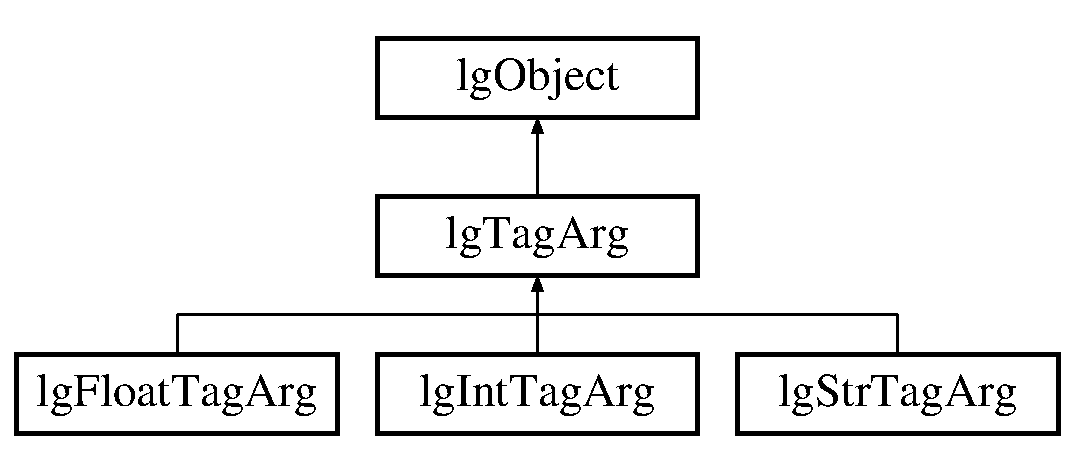
\includegraphics[height=3cm]{classlgTagArg}
\end{center}
\end{figure}
\subsection*{Public Member Functions}
\begin{CompactItemize}
\item 
virtual string {\bf to\-String} ({\bf lg\-Voice} $\ast$seq=NULL)
\item 
{\bf lg\-Tag\-Arg} (const char $\ast$na, const char $\ast$un)
\item 
virtual {\bf $\sim$lg\-Tag\-Arg} (void)
\item 
virtual string {\bf val\-Str} (void)
\item 
virtual int {\bf val\-Int} (void)
\item 
virtual double {\bf val\-Float} (void)
\item 
virtual string {\bf unit} (void)
\item 
const string {\bf name} (void)
\begin{CompactList}\small\item\em argument name, might be \char`\"{}\char`\"{} if unnamed \item\end{CompactList}\end{CompactItemize}
\subsection*{Protected Attributes}
\begin{CompactItemize}
\item 
string {\bf unit\-I}
\begin{CompactList}\small\item\em unit string, is \char`\"{}\char`\"{} for string\-Tag\-Args \item\end{CompactList}\end{CompactItemize}
\subsection*{Private Attributes}
\begin{CompactItemize}
\item 
string {\bf name\-I}
\end{CompactItemize}


\subsection{Detailed Description}
generic tag argument without value 



\subsection{Constructor \& Destructor Documentation}
\index{lgTagArg@{lg\-Tag\-Arg}!lgTagArg@{lgTagArg}}
\index{lgTagArg@{lgTagArg}!lgTagArg@{lg\-Tag\-Arg}}
\subsubsection{\setlength{\rightskip}{0pt plus 5cm}lg\-Tag\-Arg::lg\-Tag\-Arg (const char $\ast$ {\em na}, const char $\ast$ {\em un})}\label{classlgTagArg_a1}


\begin{Desc}
\item[Parameters: ]\par
\begin{description}
\item[{\em 
na}]argument name \item[{\em 
unit}]argument unit \end{description}
\end{Desc}
\index{lgTagArg@{lg\-Tag\-Arg}!~lgTagArg@{$\sim$lgTagArg}}
\index{~lgTagArg@{$\sim$lgTagArg}!lgTagArg@{lg\-Tag\-Arg}}
\subsubsection{\setlength{\rightskip}{0pt plus 5cm}lg\-Tag\-Arg::$\sim${\bf lg\-Tag\-Arg} (void)\hspace{0.3cm}{\tt  [virtual]}}\label{classlgTagArg_a2}




\subsection{Member Function Documentation}
\index{lgTagArg@{lg\-Tag\-Arg}!name@{name}}
\index{name@{name}!lgTagArg@{lg\-Tag\-Arg}}
\subsubsection{\setlength{\rightskip}{0pt plus 5cm}const string lg\-Tag\-Arg::name (void)\hspace{0.3cm}{\tt  [inline]}}\label{classlgTagArg_a7}


argument name, might be \char`\"{}\char`\"{} if unnamed 

\index{lgTagArg@{lg\-Tag\-Arg}!toString@{toString}}
\index{toString@{toString}!lgTagArg@{lg\-Tag\-Arg}}
\subsubsection{\setlength{\rightskip}{0pt plus 5cm}string lg\-Tag\-Arg::to\-String ({\bf lg\-Voice} $\ast$ {\em seq} = NULL)\hspace{0.3cm}{\tt  [virtual]}}\label{classlgTagArg_a0}


get GUIDO string should be redefined in all derived classes 

Reimplemented from {\bf lg\-Object} {\rm (p.\,\pageref{classlgObject_a3})}.

Reimplemented in {\bf lg\-Str\-Tag\-Arg} {\rm (p.\,\pageref{classlgStrTagArg_a0})}, {\bf lg\-Int\-Tag\-Arg} {\rm (p.\,\pageref{classlgIntTagArg_a0})}, and {\bf lg\-Float\-Tag\-Arg} {\rm (p.\,\pageref{classlgFloatTagArg_a0})}.\index{lgTagArg@{lg\-Tag\-Arg}!unit@{unit}}
\index{unit@{unit}!lgTagArg@{lg\-Tag\-Arg}}
\subsubsection{\setlength{\rightskip}{0pt plus 5cm}virtual string lg\-Tag\-Arg::unit (void)\hspace{0.3cm}{\tt  [inline, virtual]}}\label{classlgTagArg_a6}


\index{lgTagArg@{lg\-Tag\-Arg}!valFloat@{valFloat}}
\index{valFloat@{valFloat}!lgTagArg@{lg\-Tag\-Arg}}
\subsubsection{\setlength{\rightskip}{0pt plus 5cm}virtual double lg\-Tag\-Arg::val\-Float (void)\hspace{0.3cm}{\tt  [inline, virtual]}}\label{classlgTagArg_a5}




Reimplemented in {\bf lg\-Str\-Tag\-Arg} {\rm (p.\,\pageref{classlgStrTagArg_a5})}, {\bf lg\-Int\-Tag\-Arg} {\rm (p.\,\pageref{classlgIntTagArg_a3})}, and {\bf lg\-Float\-Tag\-Arg} {\rm (p.\,\pageref{classlgFloatTagArg_a2})}.\index{lgTagArg@{lg\-Tag\-Arg}!valInt@{valInt}}
\index{valInt@{valInt}!lgTagArg@{lg\-Tag\-Arg}}
\subsubsection{\setlength{\rightskip}{0pt plus 5cm}virtual int lg\-Tag\-Arg::val\-Int (void)\hspace{0.3cm}{\tt  [inline, virtual]}}\label{classlgTagArg_a4}




Reimplemented in {\bf lg\-Str\-Tag\-Arg} {\rm (p.\,\pageref{classlgStrTagArg_a4})}, {\bf lg\-Int\-Tag\-Arg} {\rm (p.\,\pageref{classlgIntTagArg_a2})}, and {\bf lg\-Float\-Tag\-Arg} {\rm (p.\,\pageref{classlgFloatTagArg_a4})}.\index{lgTagArg@{lg\-Tag\-Arg}!valStr@{valStr}}
\index{valStr@{valStr}!lgTagArg@{lg\-Tag\-Arg}}
\subsubsection{\setlength{\rightskip}{0pt plus 5cm}virtual string lg\-Tag\-Arg::val\-Str (void)\hspace{0.3cm}{\tt  [inline, virtual]}}\label{classlgTagArg_a3}




Reimplemented in {\bf lg\-Str\-Tag\-Arg} {\rm (p.\,\pageref{classlgStrTagArg_a3})}, {\bf lg\-Int\-Tag\-Arg} {\rm (p.\,\pageref{classlgIntTagArg_a4})}, and {\bf lg\-Float\-Tag\-Arg} {\rm (p.\,\pageref{classlgFloatTagArg_a3})}.

\subsection{Member Data Documentation}
\index{lgTagArg@{lg\-Tag\-Arg}!nameI@{nameI}}
\index{nameI@{nameI}!lgTagArg@{lg\-Tag\-Arg}}
\subsubsection{\setlength{\rightskip}{0pt plus 5cm}string {\bf lg\-Tag\-Arg::name\-I}\hspace{0.3cm}{\tt  [private]}}\label{classlgTagArg_r0}


\index{lgTagArg@{lg\-Tag\-Arg}!unitI@{unitI}}
\index{unitI@{unitI}!lgTagArg@{lg\-Tag\-Arg}}
\subsubsection{\setlength{\rightskip}{0pt plus 5cm}string {\bf lg\-Tag\-Arg::unit\-I}\hspace{0.3cm}{\tt  [protected]}}\label{classlgTagArg_p0}


unit string, is \char`\"{}\char`\"{} for string\-Tag\-Args 



The documentation for this class was generated from the following files:\begin{CompactItemize}
\item 
{\bf lgtagarg.h}\item 
{\bf lgtagarg.cpp}\end{CompactItemize}

\section{lg\-Voice Class Reference}
\label{classlgVoice}\index{lgVoice@{lgVoice}}
a GUIDO voice with list(s) for events and tags  


{\tt \#include $<$lgvoice.h$>$}

Inheritance diagram for lg\-Voice::\begin{figure}[H]
\begin{center}
\leavevmode
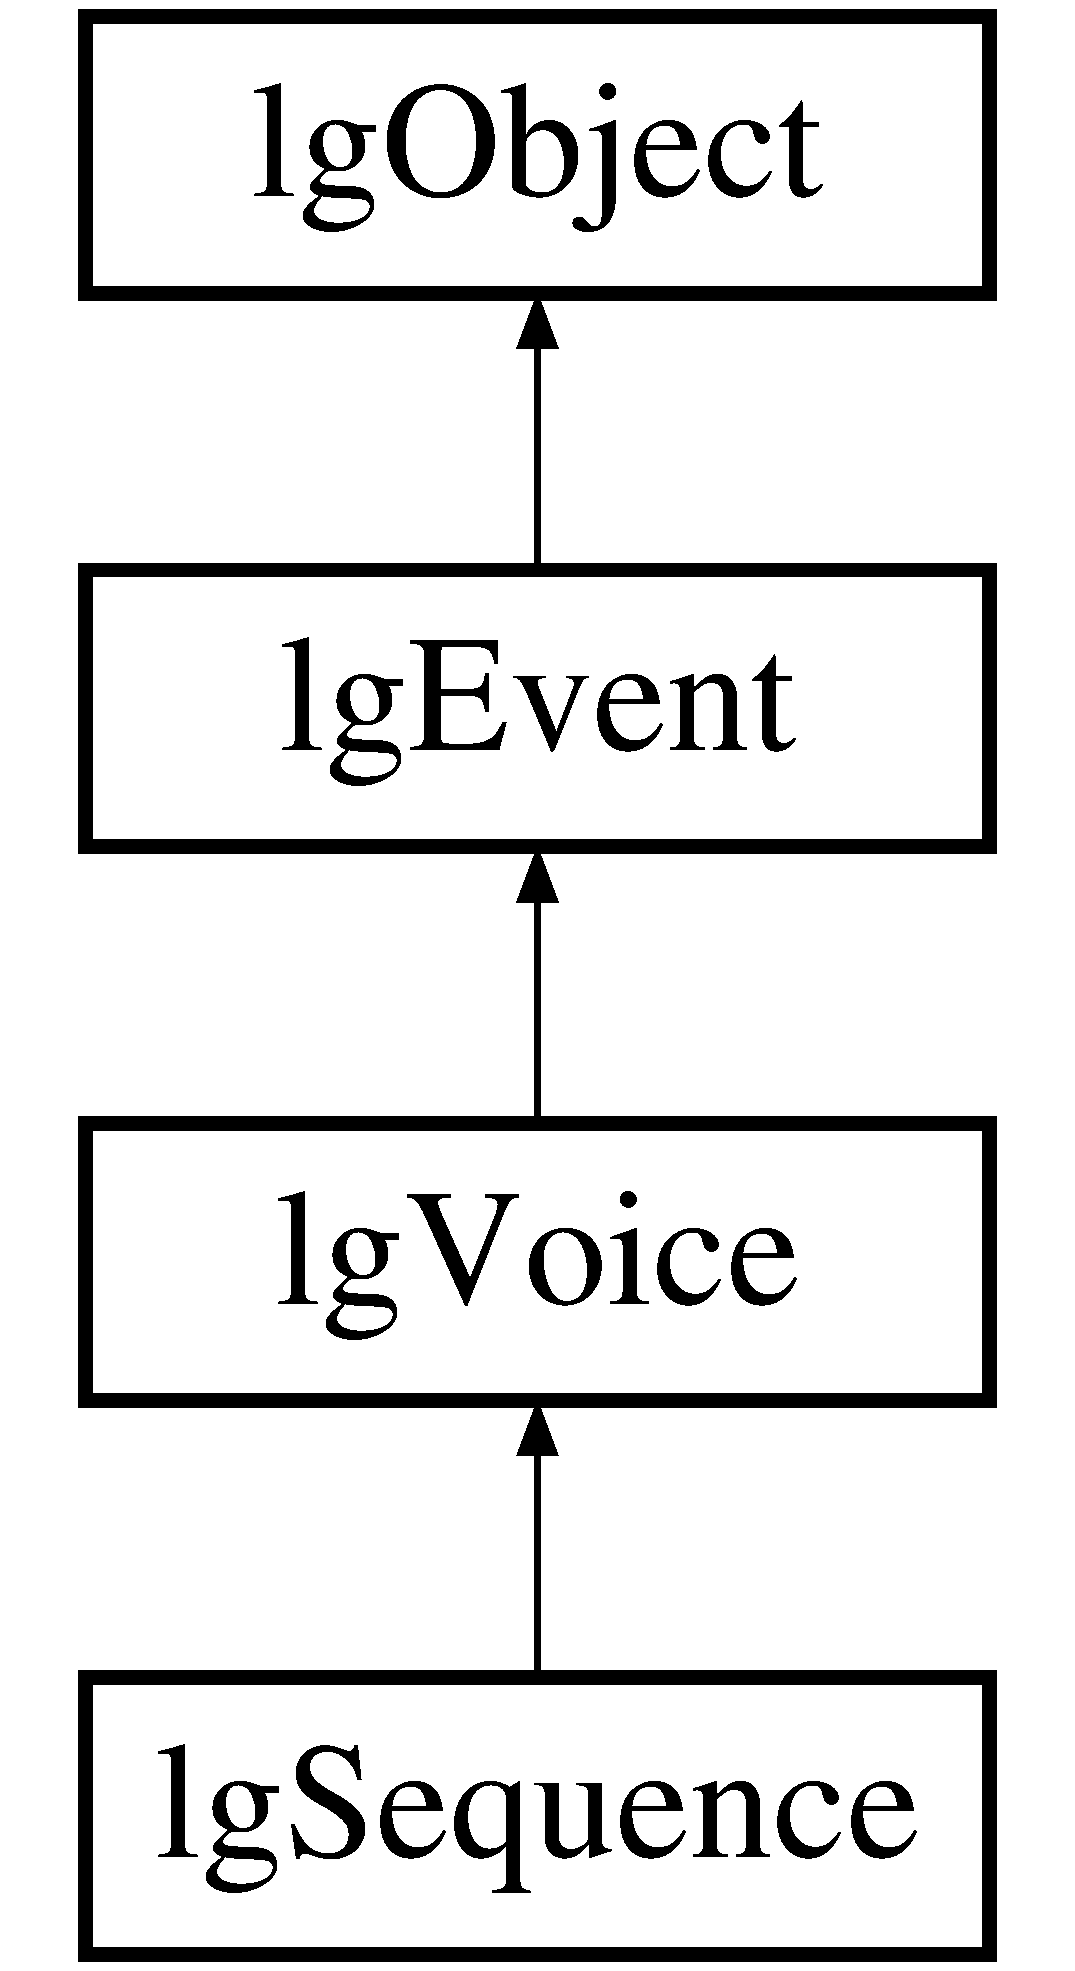
\includegraphics[height=4cm]{classlgVoice}
\end{center}
\end{figure}
\subsection*{Public Member Functions}
\begin{CompactItemize}
\item 
void {\bf replace\-Range\-Ptr} ({\bf lg\-Event} $\ast$old, {\bf lg\-Event} $\ast$new\-Ev)
\begin{CompactList}\small\item\em replace in all tags with prev\-Ev\-I==old\-Ev with new\-Ev \item\end{CompactList}\item 
virtual void {\bf set\-Next} ({\bf lg\-Voice} $\ast$seq)
\begin{CompactList}\small\item\em use also {\bf lg\-Chord::append\-Voice} as public function! \item\end{CompactList}\item 
virtual {\bf lg\-Tag} $\ast$ {\bf find\-Tag} (char $\ast$tag\-Name)
\begin{CompactList}\small\item\em search for a tag starting at beginning of the list \item\end{CompactList}\item 
virtual {\bf lg\-Tag} $\ast$ {\bf find\-Tag\-At} (const char $\ast$name, {\bf lg\-Duration} pos)
\item 
int {\bf delete\-Tag} ({\bf lg\-Tag} $\ast${\bf tag})
\begin{CompactList}\small\item\em return 1 if found \item\end{CompactList}\item 
int {\bf delete\-Event} ({\bf lg\-Event} $\ast$event)
\begin{CompactList}\small\item\em return 1 if found \item\end{CompactList}\item 
{\bf lg\-Voice} (long int pos\-Num, long int pos\-Denom)
\item 
virtual {\bf $\sim$lg\-Voice} (void)
\item 
void {\bf append\-Event} ({\bf lg\-Event} $\ast$ev)
\begin{CompactList}\small\item\em append at xx\-Tail \item\end{CompactList}\item 
void {\bf insert\-Tag} ({\bf lg\-Tag} $\ast${\bf tag})
\begin{CompactList}\small\item\em insert a tag in sorted taglist, if tag-$>$prev\-I == NULL -$>$ append at end of taglist! \item\end{CompactList}\item 
void {\bf close\-Tag} (long int no, {\bf lg\-Event} $\ast$ev, {\bf lg\-Factory} $\ast$factory)
\begin{CompactList}\small\item\em set end range of tag no \item\end{CompactList}\item 
string {\bf tags\-To\-String} ({\bf lg\-Event} $\ast$ev)
\begin{CompactList}\small\item\em write all tags between ev and ev-$>$next \item\end{CompactList}\item 
virtual {\bf lg\-Event} $\ast$ {\bf first\-Event} (void)
\begin{CompactList}\small\item\em this function doesn't look inside chords! \item\end{CompactList}\item 
virtual {\bf lg\-Event} $\ast$ {\bf next\-Event} ({\bf lg\-Event} $\ast$ev)
\begin{CompactList}\small\item\em this function doesn't look inside chords! \item\end{CompactList}\item 
virtual {\bf lg\-Note} $\ast$ {\bf first\-Note} (void)
\item 
virtual {\bf lg\-Note} $\ast$ {\bf next\-Note} ({\bf lg\-Event} $\ast$ev)
\item 
virtual long int {\bf c\-Notes} (void)
\begin{CompactList}\small\item\em return number of existing notes. Might be different to {\bf events}! \item\end{CompactList}\item 
virtual {\bf lg\-Tag} $\ast$ {\bf first\-Tag} (const char $\ast$n=NULL)
\begin{CompactList}\small\item\em get first tag with name == n \item\end{CompactList}\item 
virtual {\bf lg\-Tag} $\ast$ {\bf next\-Tag} ({\bf lg\-Tag} $\ast${\bf tag})
\item 
virtual char {\bf insert\-Event} ({\bf lg\-Event} $\ast$event)
\begin{CompactList}\small\item\em insert a event at event-$>$pos \item\end{CompactList}\item 
virtual string {\bf to\-String} ({\bf lg\-Voice} $\ast$calling\-Seq=NULL)
\item 
virtual void {\bf write} (FILE $\ast$out, {\bf lg\-Voice} $\ast$v=NULL)
\begin{CompactList}\small\item\em write to .gmn \item\end{CompactList}\item 
virtual lg\-Frac {\bf duration} (void)
\begin{CompactList}\small\item\em return duration of voice, events\-Tail must be uptodate! \item\end{CompactList}\item 
virtual {\bf lg\-Tag} $\ast$ {\bf find\-Tag} (long int id)
\begin{CompactList}\small\item\em search for tag in tag list and all chords \item\end{CompactList}\item 
virtual {\bf lg\-Event} $\ast$ {\bf find\-Event} ({\bf lg\-Duration} at\-Pos)
\begin{CompactList}\small\item\em search for event with event-$>$pos == at\-Pos, return NULL if not found \item\end{CompactList}\item 
{\bf lg\-Event} $\ast$ {\bf event\-Hold\-At} ({\bf lg\-Duration} pos)
\begin{CompactList}\small\item\em check if an event is holding at pos \item\end{CompactList}\item 
{\bf lg\-Event} $\ast$ {\bf latest\-Eventbefore} ({\bf lg\-Duration} pos)
\begin{CompactList}\small\item\em get latest event ending $<$= pos \item\end{CompactList}\item 
char {\bf split\-Event} ({\bf lg\-Duration} pos)
\item 
void {\bf insert\-Tag} ({\bf lg\-Tag} $\ast${\bf tag}, {\bf lg\-Duration} start\-Range, {\bf lg\-Duration} end\-Range)
\item 
int {\bf split\-Tag\-Ranges} (void)
\end{CompactItemize}
\subsection*{Private Attributes}
\begin{CompactItemize}
\item 
{\bf lg\-Event} $\ast$ {\bf events}
\begin{CompactList}\small\item\em event list \item\end{CompactList}\item 
{\bf lg\-Event} $\ast$ {\bf events\-Tail}
\begin{CompactList}\small\item\em event list \item\end{CompactList}\item 
{\bf lg\-Tag} $\ast$ {\bf tags}
\begin{CompactList}\small\item\em tag list \item\end{CompactList}\item 
{\bf lg\-Tag} $\ast$ {\bf tags\-Tail}
\begin{CompactList}\small\item\em tag list \item\end{CompactList}\item 
{\bf lg\-Chord} $\ast$ {\bf parent}
\begin{CompactList}\small\item\em usually this is a segment or a chord \item\end{CompactList}\end{CompactItemize}
\subsection*{Friends}
\begin{CompactItemize}
\item 
class {\bf lg\-Chord}
\begin{CompactList}\small\item\em type can be Sequence or voice (= chord voice ) \item\end{CompactList}\item 
class {\bf lg\-Segment}
\begin{CompactList}\small\item\em allow to call set\-Next \item\end{CompactList}\end{CompactItemize}


\subsection{Detailed Description}
a GUIDO voice with list(s) for events and tags 

lg\-Voice includes no cur\-Event, cur\-Tag pointers for memory saving reasons! if a lg\-Seqeunce includes a large number of chords which then inlcude lg\-Voice data the memory size would be unneccessary blown up. 



\subsection{Constructor \& Destructor Documentation}
\index{lgVoice@{lg\-Voice}!lgVoice@{lgVoice}}
\index{lgVoice@{lgVoice}!lgVoice@{lg\-Voice}}
\subsubsection{\setlength{\rightskip}{0pt plus 5cm}lg\-Voice::lg\-Voice (long int {\em pos\-Num}, long int {\em pos\-Denom})}\label{classlgVoice_a6}


\index{lgVoice@{lg\-Voice}!~lgVoice@{$\sim$lgVoice}}
\index{~lgVoice@{$\sim$lgVoice}!lgVoice@{lg\-Voice}}
\subsubsection{\setlength{\rightskip}{0pt plus 5cm}lg\-Voice::$\sim${\bf lg\-Voice} (void)\hspace{0.3cm}{\tt  [virtual]}}\label{classlgVoice_a7}


delete all events

delete all tags 

\subsection{Member Function Documentation}
\index{lgVoice@{lg\-Voice}!appendEvent@{appendEvent}}
\index{appendEvent@{appendEvent}!lgVoice@{lg\-Voice}}
\subsubsection{\setlength{\rightskip}{0pt plus 5cm}void lg\-Voice::append\-Event ({\bf lg\-Event} $\ast$ {\em ev})}\label{classlgVoice_a8}


append at xx\-Tail 

\index{lgVoice@{lg\-Voice}!closeTag@{closeTag}}
\index{closeTag@{closeTag}!lgVoice@{lg\-Voice}}
\subsubsection{\setlength{\rightskip}{0pt plus 5cm}void lg\-Voice::close\-Tag (long int {\em no}, {\bf lg\-Event} $\ast$ {\em ev}, {\bf lg\-Factory} $\ast$ {\em factory})}\label{classlgVoice_a10}


set end range of tag no 

this might be needed for nested scores in Extended GUIDO void append\-Segment(lg\-Segment $\ast$seg); //! append at xx\-Tail \index{lgVoice@{lg\-Voice}!cNotes@{cNotes}}
\index{cNotes@{cNotes}!lgVoice@{lg\-Voice}}
\subsubsection{\setlength{\rightskip}{0pt plus 5cm}long int lg\-Voice::c\-Notes (void)\hspace{0.3cm}{\tt  [virtual]}}\label{classlgVoice_a16}


return number of existing notes. Might be different to {\bf events}! 

\index{lgVoice@{lg\-Voice}!deleteEvent@{deleteEvent}}
\index{deleteEvent@{deleteEvent}!lgVoice@{lg\-Voice}}
\subsubsection{\setlength{\rightskip}{0pt plus 5cm}int lg\-Voice::delete\-Event ({\bf lg\-Event} $\ast$ {\em ev})}\label{classlgVoice_a5}


return 1 if found 

search for event \index{lgVoice@{lg\-Voice}!deleteTag@{deleteTag}}
\index{deleteTag@{deleteTag}!lgVoice@{lg\-Voice}}
\subsubsection{\setlength{\rightskip}{0pt plus 5cm}int lg\-Voice::delete\-Tag ({\bf lg\-Tag} $\ast$ {\em tag})}\label{classlgVoice_a4}


return 1 if found 

remove head of list? \index{lgVoice@{lg\-Voice}!duration@{duration}}
\index{duration@{duration}!lgVoice@{lg\-Voice}}
\subsubsection{\setlength{\rightskip}{0pt plus 5cm}{\bf lg\-Duration} lg\-Voice::duration (void)\hspace{0.3cm}{\tt  [virtual]}}\label{classlgVoice_a22}


return duration of voice, events\-Tail must be uptodate! 

return duration of a voice events\-Tail must be up to date! 

Reimplemented from {\bf lg\-Event} {\rm (p.\,\pageref{classlgEvent_a2})}.\index{lgVoice@{lg\-Voice}!eventHoldAt@{eventHoldAt}}
\index{eventHoldAt@{eventHoldAt}!lgVoice@{lg\-Voice}}
\subsubsection{\setlength{\rightskip}{0pt plus 5cm}{\bf lg\-Event}$\ast$ lg\-Voice::event\-Hold\-At ({\bf lg\-Duration} {\em pos})}\label{classlgVoice_a25}


check if an event is holding at pos 

\index{lgVoice@{lg\-Voice}!findEvent@{findEvent}}
\index{findEvent@{findEvent}!lgVoice@{lg\-Voice}}
\subsubsection{\setlength{\rightskip}{0pt plus 5cm}{\bf lg\-Event} $\ast$ lg\-Voice::find\-Event ({\bf lg\-Duration} {\em at\-Pos})\hspace{0.3cm}{\tt  [virtual]}}\label{classlgVoice_a24}


search for event with event-$>$pos == at\-Pos, return NULL if not found 

\index{lgVoice@{lg\-Voice}!findTag@{findTag}}
\index{findTag@{findTag}!lgVoice@{lg\-Voice}}
\subsubsection{\setlength{\rightskip}{0pt plus 5cm}{\bf lg\-Tag} $\ast$ lg\-Voice::find\-Tag (long int {\em id})\hspace{0.3cm}{\tt  [virtual]}}\label{classlgVoice_a23}


search for tag in tag list and all chords 

search in tag list

search in chords! \index{lgVoice@{lg\-Voice}!findTag@{findTag}}
\index{findTag@{findTag}!lgVoice@{lg\-Voice}}
\subsubsection{\setlength{\rightskip}{0pt plus 5cm}{\bf lg\-Tag} $\ast$ lg\-Voice::find\-Tag (char $\ast$ {\em tag\-Name})\hspace{0.3cm}{\tt  [virtual]}}\label{classlgVoice_a2}


search for a tag starting at beginning of the list 

search in tag list

search in chords! \index{lgVoice@{lg\-Voice}!findTagAt@{findTagAt}}
\index{findTagAt@{findTagAt}!lgVoice@{lg\-Voice}}
\subsubsection{\setlength{\rightskip}{0pt plus 5cm}{\bf lg\-Tag} $\ast$ lg\-Voice::find\-Tag\-At (const char $\ast$ {\em name}, {\bf lg\-Duration} {\em pos})\hspace{0.3cm}{\tt  [virtual]}}\label{classlgVoice_a3}


get tag which is valid at position pos a tag is valid if pos is inside range or no range is specified this function does not look inside chords! \index{lgVoice@{lg\-Voice}!firstEvent@{firstEvent}}
\index{firstEvent@{firstEvent}!lgVoice@{lg\-Voice}}
\subsubsection{\setlength{\rightskip}{0pt plus 5cm}{\bf lg\-Event} $\ast$ lg\-Voice::first\-Event (void)\hspace{0.3cm}{\tt  [virtual]}}\label{classlgVoice_a12}


this function doesn't look inside chords! 

\index{lgVoice@{lg\-Voice}!firstNote@{firstNote}}
\index{firstNote@{firstNote}!lgVoice@{lg\-Voice}}
\subsubsection{\setlength{\rightskip}{0pt plus 5cm}virtual {\bf lg\-Note}$\ast$ lg\-Voice::first\-Note (void)\hspace{0.3cm}{\tt  [inline, virtual]}}\label{classlgVoice_a14}


\index{lgVoice@{lg\-Voice}!firstTag@{firstTag}}
\index{firstTag@{firstTag}!lgVoice@{lg\-Voice}}
\subsubsection{\setlength{\rightskip}{0pt plus 5cm}{\bf lg\-Tag} $\ast$ lg\-Voice::first\-Tag (const char $\ast$ {\em n} = NULL)\hspace{0.3cm}{\tt  [virtual]}}\label{classlgVoice_a17}


get first tag with name == n 

\index{lgVoice@{lg\-Voice}!insertEvent@{insertEvent}}
\index{insertEvent@{insertEvent}!lgVoice@{lg\-Voice}}
\subsubsection{\setlength{\rightskip}{0pt plus 5cm}char lg\-Voice::insert\-Event ({\bf lg\-Event} $\ast$ {\em event})\hspace{0.3cm}{\tt  [virtual]}}\label{classlgVoice_a19}


insert a event at event-$>$pos 

pos of succeeding events must be recalced! return 1: ok 0 : can not be inserted because of collision with existing events\index{lgVoice@{lg\-Voice}!insertTag@{insertTag}}
\index{insertTag@{insertTag}!lgVoice@{lg\-Voice}}
\subsubsection{\setlength{\rightskip}{0pt plus 5cm}void lg\-Voice::insert\-Tag ({\bf lg\-Tag} $\ast$ {\em tag}, {\bf lg\-Duration} {\em start\-Range}, {\bf lg\-Duration} {\em end\-Range})}\label{classlgVoice_a28}


insert a tag and set range pointers of tag holding events will be splitted if start\-Range==end\-Range no range will be set \index{lgVoice@{lg\-Voice}!insertTag@{insertTag}}
\index{insertTag@{insertTag}!lgVoice@{lg\-Voice}}
\subsubsection{\setlength{\rightskip}{0pt plus 5cm}void lg\-Voice::insert\-Tag ({\bf lg\-Tag} $\ast$ {\em tag})}\label{classlgVoice_a9}


insert a tag in sorted taglist, if tag-$>$prev\-I == NULL -$>$ append at end of taglist! 

insert tag in tag list keep tag normal form uptodate! if tag1-$>$pos == tag2-$>$pos unranged tags will sorted first \index{lgVoice@{lg\-Voice}!latestEventbefore@{latestEventbefore}}
\index{latestEventbefore@{latestEventbefore}!lgVoice@{lg\-Voice}}
\subsubsection{\setlength{\rightskip}{0pt plus 5cm}{\bf lg\-Event}$\ast$ lg\-Voice::latest\-Eventbefore ({\bf lg\-Duration} {\em pos})}\label{classlgVoice_a26}


get latest event ending $<$= pos 

\index{lgVoice@{lg\-Voice}!nextEvent@{nextEvent}}
\index{nextEvent@{nextEvent}!lgVoice@{lg\-Voice}}
\subsubsection{\setlength{\rightskip}{0pt plus 5cm}{\bf lg\-Event} $\ast$ lg\-Voice::next\-Event ({\bf lg\-Event} $\ast$ {\em ev})\hspace{0.3cm}{\tt  [virtual]}}\label{classlgVoice_a13}


this function doesn't look inside chords! 

\index{lgVoice@{lg\-Voice}!nextNote@{nextNote}}
\index{nextNote@{nextNote}!lgVoice@{lg\-Voice}}
\subsubsection{\setlength{\rightskip}{0pt plus 5cm}virtual {\bf lg\-Note}$\ast$ lg\-Voice::next\-Note ({\bf lg\-Event} $\ast$ {\em ev})\hspace{0.3cm}{\tt  [inline, virtual]}}\label{classlgVoice_a15}


\index{lgVoice@{lg\-Voice}!nextTag@{nextTag}}
\index{nextTag@{nextTag}!lgVoice@{lg\-Voice}}
\subsubsection{\setlength{\rightskip}{0pt plus 5cm}{\bf lg\-Tag} $\ast$ lg\-Voice::next\-Tag ({\bf lg\-Tag} $\ast$ {\em tag})\hspace{0.3cm}{\tt  [virtual]}}\label{classlgVoice_a18}


\index{lgVoice@{lg\-Voice}!replaceRangePtr@{replaceRangePtr}}
\index{replaceRangePtr@{replaceRangePtr}!lgVoice@{lg\-Voice}}
\subsubsection{\setlength{\rightskip}{0pt plus 5cm}void lg\-Voice::replace\-Range\-Ptr ({\bf lg\-Event} $\ast$ {\em old}, {\bf lg\-Event} $\ast$ {\em new\-Ev})}\label{classlgVoice_a0}


replace in all tags with prev\-Ev\-I==old\-Ev with new\-Ev 

\index{lgVoice@{lg\-Voice}!setNext@{setNext}}
\index{setNext@{setNext}!lgVoice@{lg\-Voice}}
\subsubsection{\setlength{\rightskip}{0pt plus 5cm}void lg\-Voice::set\-Next ({\bf lg\-Voice} $\ast$ {\em seq})\hspace{0.3cm}{\tt  [virtual]}}\label{classlgVoice_a1}


use also {\bf lg\-Chord::append\-Voice} as public function! 

\index{lgVoice@{lg\-Voice}!splitEvent@{splitEvent}}
\index{splitEvent@{splitEvent}!lgVoice@{lg\-Voice}}
\subsubsection{\setlength{\rightskip}{0pt plus 5cm}char lg\-Voice::split\-Event ({\bf lg\-Duration} {\em pos})}\label{classlgVoice_a27}


slit an event and tie if needed return 0 if no event needed to be split \index{lgVoice@{lg\-Voice}!splitTagRanges@{splitTagRanges}}
\index{splitTagRanges@{splitTagRanges}!lgVoice@{lg\-Voice}}
\subsubsection{\setlength{\rightskip}{0pt plus 5cm}int lg\-Voice::split\-Tag\-Ranges (void)}\label{classlgVoice_a29}


split all explicit tag ranges (using \char`\"{}(....\char`\"{}) ) into $\backslash$...Begin and $\backslash$...End, return number of splittedt ranges \index{lgVoice@{lg\-Voice}!tagsToString@{tagsToString}}
\index{tagsToString@{tagsToString}!lgVoice@{lg\-Voice}}
\subsubsection{\setlength{\rightskip}{0pt plus 5cm}string lg\-Voice::tags\-To\-String ({\bf lg\-Event} $\ast$ {\em ev})}\label{classlgVoice_a11}


write all tags between ev and ev-$>$next 

all tags, located between ev and ev-$>$next if ev == lg\-Voice get all tags at beginning of voice \index{lgVoice@{lg\-Voice}!toString@{toString}}
\index{toString@{toString}!lgVoice@{lg\-Voice}}
\subsubsection{\setlength{\rightskip}{0pt plus 5cm}string lg\-Voice::to\-String ({\bf lg\-Voice} $\ast$ {\em call\-Seq} = NULL)\hspace{0.3cm}{\tt  [virtual]}}\label{classlgVoice_a20}


tags at beginn of the voice 

write event

write all tags after event 

Reimplemented from {\bf lg\-Event} {\rm (p.\,\pageref{classlgEvent_a1})}.

Reimplemented in {\bf lg\-Sequence} {\rm (p.\,\pageref{classlgSequence_a0})}.\index{lgVoice@{lg\-Voice}!write@{write}}
\index{write@{write}!lgVoice@{lg\-Voice}}
\subsubsection{\setlength{\rightskip}{0pt plus 5cm}void lg\-Voice::write (FILE $\ast$ {\em out}, {\bf lg\-Voice} $\ast$ {\em v} = NULL)\hspace{0.3cm}{\tt  [virtual]}}\label{classlgVoice_a21}


write to .gmn 

could be replaced by 

Reimplemented from {\bf lg\-Event} {\rm (p.\,\pageref{classlgEvent_a8})}.

\subsection{Friends And Related Function Documentation}
\index{lgVoice@{lg\-Voice}!lgChord@{lgChord}}
\index{lgChord@{lgChord}!lgVoice@{lg\-Voice}}
\subsubsection{\setlength{\rightskip}{0pt plus 5cm}friend class {\bf lg\-Chord}\hspace{0.3cm}{\tt  [friend]}}\label{classlgVoice_n0}


type can be Sequence or voice (= chord voice ) 



Reimplemented from {\bf lg\-Event} {\rm (p.\,\pageref{classlgEvent_n1})}.\index{lgVoice@{lg\-Voice}!lgSegment@{lgSegment}}
\index{lgSegment@{lgSegment}!lgVoice@{lg\-Voice}}
\subsubsection{\setlength{\rightskip}{0pt plus 5cm}friend class {\bf lg\-Segment}\hspace{0.3cm}{\tt  [friend]}}\label{classlgVoice_n1}


allow to call set\-Next 



Reimplemented from {\bf lg\-Object} {\rm (p.\,\pageref{classlgObject_n3})}.

\subsection{Member Data Documentation}
\index{lgVoice@{lg\-Voice}!events@{events}}
\index{events@{events}!lgVoice@{lg\-Voice}}
\subsubsection{\setlength{\rightskip}{0pt plus 5cm}{\bf lg\-Event}$\ast$ {\bf lg\-Voice::events}\hspace{0.3cm}{\tt  [private]}}\label{classlgVoice_r0}


event list 

\index{lgVoice@{lg\-Voice}!eventsTail@{eventsTail}}
\index{eventsTail@{eventsTail}!lgVoice@{lg\-Voice}}
\subsubsection{\setlength{\rightskip}{0pt plus 5cm}{\bf lg\-Event} $\ast$ {\bf lg\-Voice::events\-Tail}\hspace{0.3cm}{\tt  [private]}}\label{classlgVoice_r1}


event list 

\index{lgVoice@{lg\-Voice}!parent@{parent}}
\index{parent@{parent}!lgVoice@{lg\-Voice}}
\subsubsection{\setlength{\rightskip}{0pt plus 5cm}{\bf lg\-Chord}$\ast$ {\bf lg\-Voice::parent}\hspace{0.3cm}{\tt  [private]}}\label{classlgVoice_r4}


usually this is a segment or a chord 

\index{lgVoice@{lg\-Voice}!tags@{tags}}
\index{tags@{tags}!lgVoice@{lg\-Voice}}
\subsubsection{\setlength{\rightskip}{0pt plus 5cm}{\bf lg\-Tag}$\ast$ {\bf lg\-Voice::tags}\hspace{0.3cm}{\tt  [private]}}\label{classlgVoice_r2}


tag list 

\index{lgVoice@{lg\-Voice}!tagsTail@{tagsTail}}
\index{tagsTail@{tagsTail}!lgVoice@{lg\-Voice}}
\subsubsection{\setlength{\rightskip}{0pt plus 5cm}{\bf lg\-Tag} $\ast$ {\bf lg\-Voice::tags\-Tail}\hspace{0.3cm}{\tt  [private]}}\label{classlgVoice_r3}


tag list 



The documentation for this class was generated from the following files:\begin{CompactItemize}
\item 
{\bf lgvoice.h}\item 
{\bf lgvoice.cpp}\end{CompactItemize}

\section{string\-Visitor Class Reference}
\label{classstringVisitor}\index{stringVisitor@{stringVisitor}}
prototype for a string visitor, not really used at the moment  


{\tt \#include $<$lgvisitor.h$>$}

\subsection*{Public Member Functions}
\begin{CompactItemize}
\item 
string {\bf visit} ({\bf lg\-Object} $\ast$o)
\item 
string {\bf visit} ({\bf lg\-Event} $\ast$e)
\item 
string {\bf visit} ({\bf lg\-Tag} $\ast$t)
\end{CompactItemize}


\subsection{Detailed Description}
prototype for a string visitor, not really used at the moment 



\subsection{Member Function Documentation}
\index{stringVisitor@{string\-Visitor}!visit@{visit}}
\index{visit@{visit}!stringVisitor@{string\-Visitor}}
\subsubsection{\setlength{\rightskip}{0pt plus 5cm}string string\-Visitor::visit ({\bf lg\-Tag} $\ast$ {\em t})}\label{classstringVisitor_a2}


\index{stringVisitor@{string\-Visitor}!visit@{visit}}
\index{visit@{visit}!stringVisitor@{string\-Visitor}}
\subsubsection{\setlength{\rightskip}{0pt plus 5cm}string string\-Visitor::visit ({\bf lg\-Event} $\ast$ {\em e})}\label{classstringVisitor_a1}


\index{stringVisitor@{string\-Visitor}!visit@{visit}}
\index{visit@{visit}!stringVisitor@{string\-Visitor}}
\subsubsection{\setlength{\rightskip}{0pt plus 5cm}string string\-Visitor::visit ({\bf lg\-Object} $\ast$ {\em o})}\label{classstringVisitor_a0}




The documentation for this class was generated from the following files:\begin{CompactItemize}
\item 
{\bf lgvisitor.h}\item 
{\bf lgvisitor.cpp}\end{CompactItemize}

\section{strlist Struct Reference}
\label{structstrlist}\index{strlist@{strlist}}
{\tt \#include $<$strlist.h$>$}

\subsection*{Public Attributes}
\begin{CompactItemize}
\item 
char $\ast$ {\bf table} [100]
\item 
int {\bf length}
\end{CompactItemize}


\subsection{Member Data Documentation}
\index{strlist@{strlist}!length@{length}}
\index{length@{length}!strlist@{strlist}}
\subsubsection{\setlength{\rightskip}{0pt plus 5cm}int {\bf strlist::length}}\label{structstrlist_o1}


\index{strlist@{strlist}!table@{table}}
\index{table@{table}!strlist@{strlist}}
\subsubsection{\setlength{\rightskip}{0pt plus 5cm}char$\ast$ {\bf strlist::table}[100]}\label{structstrlist_o0}




The documentation for this struct was generated from the following file:\begin{CompactItemize}
\item 
{\bf strlist.h}\end{CompactItemize}

\section{tag\-Stack Struct Reference}
\label{structtagStack}\index{tagStack@{tagStack}}
\subsection*{Public Attributes}
\begin{CompactItemize}
\item 
long int {\bf tagno}
\item 
void $\ast$ {\bf next}
\end{CompactItemize}


\subsection{Member Data Documentation}
\index{tagStack@{tag\-Stack}!next@{next}}
\index{next@{next}!tagStack@{tag\-Stack}}
\subsubsection{\setlength{\rightskip}{0pt plus 5cm}void$\ast$ {\bf tag\-Stack::next}}\label{structtagStack_o1}


\index{tagStack@{tag\-Stack}!tagno@{tagno}}
\index{tagno@{tagno}!tagStack@{tag\-Stack}}
\subsubsection{\setlength{\rightskip}{0pt plus 5cm}long int {\bf tag\-Stack::tagno}}\label{structtagStack_o0}




The documentation for this struct was generated from the following file:\begin{CompactItemize}
\item 
{\bf guido.cpp}\end{CompactItemize}

\chapter{lean\-GUIDO File Documentation}
\section{duration.cpp File Reference}
\label{duration_8cpp}\index{duration.cpp@{duration.cpp}}
{\tt \#include $<$sstream$>$}\par
{\tt \#include \char`\"{}duration.h\char`\"{}}\par

\section{duration.h File Reference}
\label{duration_8h}\index{duration.h@{duration.h}}
{\tt \#include $<$stdio.h$>$}\par
{\tt \#include $<$string$>$}\par
\subsection*{Namespaces}
\begin{CompactItemize}
\item 
namespace {\bf std}
\end{CompactItemize}
\subsection*{Compounds}
\begin{CompactItemize}
\item 
class {\bf lg\-Duration}
\begin{CompactList}\small\item\em generic fraction class. lg\-Duration is used to store the information pertaining to the duration/attacktime of a note. \item\end{CompactList}\end{CompactItemize}

\section{guido.cpp File Reference}
\label{guido_8cpp}\index{guido.cpp@{guido.cpp}}
{\tt \#include \char`\"{}guido.h\char`\"{}}\par
{\tt \#include \char`\"{}parser\_\-t.c\char`\"{}}\par
{\tt \#include \char`\"{}strlist.h\char`\"{}}\par
{\tt \#include \char`\"{}naguido.h\char`\"{}}\par
\subsection*{Compounds}
\begin{CompactItemize}
\item 
struct {\bf ARGV}
\item 
struct {\bf tag\-Stack}
\end{CompactItemize}
\subsection*{Defines}
\begin{CompactItemize}
\item 
\#define {\bf DEBUG}(x)
\end{CompactItemize}
\subsection*{Functions}
\begin{CompactItemize}
\item 
void {\bf gd\_\-init} (void)
\item 
void {\bf gd\_\-exit} (void)
\item 
int {\bf gd\_\-parse} (const char $\ast$filename, int mode)
\item 
void {\bf gd\_\-frac\-Norm} (long int $\ast$a, long int $\ast$b)
\item 
void {\bf gd\_\-frac\-Add} (long int $\ast$a, long int $\ast$b, const long int c, const long int d)
\item 
int {\bf gd\_\-frac\-Cmp} (long int a, long int b, long int c, long int d)
\item 
long int {\bf gd\_\-tag\-Stack\-Pop} (void)
\item 
void {\bf gd\_\-tag\-Stack\-Clear} (void)
\item 
void {\bf gd\_\-tag\-Stack\-Push} (long int {\bf tagno})
\item 
int {\bf gd\_\-note\-Name2pc} (char $\ast$name)
\item 
void {\bf gd\_\-note\-Init} (char $\ast$id)
\item 
void {\bf gd\_\-note\-Acc} (int n)
\item 
void {\bf gd\_\-note\-Oct} (int n)
\item 
void {\bf gd\_\-note\-Enum} (long int n)
\item 
void {\bf gd\_\-note\-Denom} (long int n)
\item 
void {\bf gd\_\-note\-Dot} (void)
\item 
void {\bf gd\_\-note\-Ddot} (void)
\item 
void {\bf gd\_\-note\-Abs\-Dur} (long int n)
\item 
void {\bf gd\_\-seq\-Append\-Note} (void)
\item 
void {\bf gd\_\-chord\-Init} (void)
\item 
void {\bf gd\_\-chord\-Init\-Note} (void)
\item 
void {\bf gd\_\-chord\-Append\-Note} (void)
\item 
void {\bf gd\_\-seq\-Append\-Chord} (void)
\item 
void {\bf gd\_\-seq\-Init} (void)
\item 
void {\bf gd\_\-seq\-Exit} (void)
\item 
void {\bf gd\_\-segm\-Init} (void)
\item 
void {\bf gd\_\-segm\-Exit} (void)
\item 
void {\bf gd\_\-segm\-Append\-Seq} (void)
\item 
void {\bf gd\_\-tag\-Start} (char $\ast$id, long int no)
\item 
void {\bf gd\_\-tag\-End} (void)
\item 
void {\bf gd\_\-tag\-Int\-Arg} (long int n)
\item 
void {\bf gd\_\-tag\-Float\-Arg} (T\_\-REAL r)
\item 
void {\bf gd\_\-tag\-Arg\-Unit} (char $\ast$unit)
\item 
void {\bf gd\_\-tag\-Str\-Arg} (char $\ast$s)
\item 
void {\bf gd\_\-tag\-Add\-Arg} (char $\ast$s)
\item 
void {\bf gd\_\-tag\-Add} (void)
\item 
void {\bf gd\_\-tag\-Range} (void)
\item 
char {\bf gd\_\-get\-Tag\-Arg\-Type} (int n)
\item 
char $\ast$ {\bf gd\_\-get\-Tag\-Arg\-Name} (int n)
\item 
long int {\bf gd\_\-get\-Tag\-Arg\-Int} (int n)
\item 
T\_\-REAL {\bf gd\_\-get\-Tag\-Arg\-Float} (int n)
\item 
char $\ast$ {\bf gd\_\-get\-Tag\-Arg\-Unit} (int n)
\item 
char $\ast$ {\bf gd\_\-get\-Tag\-Arg\-Str} (int n)
\item 
void {\bf gd\_\-dur\-Incr\-On} (void)
\item 
void {\bf gd\_\-dur\-Incr\-Off} (void)
\item 
int {\bf gd\_\-error} (const char $\ast$msg)
\end{CompactItemize}
\subsection*{Variables}
\begin{CompactItemize}
\item 
int {\bf parse\_\-mode}
\item 
long int {\bf lnr}
\item 
long int {\bf cnr}
\item 
long int {\bf cmnt\_\-level}
\item 
long int {\bf tagno}
\item 
long int {\bf this\_\-tagno}
\item 
{\bf tag\-Stack} $\ast$ {\bf tag\-Stack\-Top} = NULL
\item 
int {\bf rtp\_\-auto\_\-inc} = 1
\item 
long int {\bf sg\_\-num\_\-voices} = 0
\item 
long int {\bf sg\_\-num\_\-notes} = 0
\item 
long int {\bf sg\_\-num\_\-tags} = 0
\item 
long int {\bf sg\_\-enum} = 0
\item 
long int {\bf sg\_\-denom} = 1
\item 
long int {\bf sq\_\-num\_\-notes} = 0
\item 
long int {\bf sq\_\-num\_\-tags} = 0
\item 
long int {\bf sq\_\-max\_\-voices} = 0
\item 
long int {\bf rtp\_\-enum} = 0
\item 
long int {\bf rtp\_\-denom} = 1
\item 
long int {\bf last\_\-rtp\_\-enum} = 0
\item 
long int {\bf last\_\-rtp\_\-denom} = 1
\item 
long int {\bf rtp\_\-ch\_\-enum} = 0
\item 
long int {\bf rtp\_\-ch\_\-denom} = 1
\item 
int {\bf nt\_\-dot\-Mode} = 0
\item 
int {\bf nt\_\-enum\-Set} = 0
\item 
int {\bf nt\_\-abs\-Dur\-Mode} = 0
\item 
int {\bf nt\_\-pc} = 0
\item 
int {\bf nt\_\-oct} = 1
\item 
int {\bf nt\_\-acc} = 0
\item 
long int {\bf nt\_\-enum} = 0
\item 
long int {\bf nt\_\-denom} = 1
\item 
int {\bf ch\_\-num\_\-notes} = 0
\item 
long int {\bf ch\_\-enum} = 0
\item 
long int {\bf ch\_\-denom} = 1
\item 
char $\ast$ {\bf tag}
\item 
int {\bf argc}
\item 
{\bf ARGV} $\ast$ {\bf argv}
\end{CompactItemize}


\subsection{Define Documentation}
\index{guido.cpp@{guido.cpp}!DEBUG@{DEBUG}}
\index{DEBUG@{DEBUG}!guido.cpp@{guido.cpp}}
\subsubsection{\setlength{\rightskip}{0pt plus 5cm}\#define DEBUG(x)}\label{guido_8cpp_a0}




\subsection{Function Documentation}
\index{guido.cpp@{guido.cpp}!gd_chordAppendNote@{gd\_\-chordAppendNote}}
\index{gd_chordAppendNote@{gd\_\-chordAppendNote}!guido.cpp@{guido.cpp}}
\subsubsection{\setlength{\rightskip}{0pt plus 5cm}void gd\_\-chord\-Append\-Note (void)}\label{guido_8cpp_a58}


\index{guido.cpp@{guido.cpp}!gd_chordInit@{gd\_\-chordInit}}
\index{gd_chordInit@{gd\_\-chordInit}!guido.cpp@{guido.cpp}}
\subsubsection{\setlength{\rightskip}{0pt plus 5cm}void gd\_\-chord\-Init (void)}\label{guido_8cpp_a56}


\index{guido.cpp@{guido.cpp}!gd_chordInitNote@{gd\_\-chordInitNote}}
\index{gd_chordInitNote@{gd\_\-chordInitNote}!guido.cpp@{guido.cpp}}
\subsubsection{\setlength{\rightskip}{0pt plus 5cm}void gd\_\-chord\-Init\-Note (void)}\label{guido_8cpp_a57}


\index{guido.cpp@{guido.cpp}!gd_durIncrOff@{gd\_\-durIncrOff}}
\index{gd_durIncrOff@{gd\_\-durIncrOff}!guido.cpp@{guido.cpp}}
\subsubsection{\setlength{\rightskip}{0pt plus 5cm}void gd\_\-dur\-Incr\-Off (void)}\label{guido_8cpp_a81}


\index{guido.cpp@{guido.cpp}!gd_durIncrOn@{gd\_\-durIncrOn}}
\index{gd_durIncrOn@{gd\_\-durIncrOn}!guido.cpp@{guido.cpp}}
\subsubsection{\setlength{\rightskip}{0pt plus 5cm}void gd\_\-dur\-Incr\-On (void)}\label{guido_8cpp_a80}


\index{guido.cpp@{guido.cpp}!gd_error@{gd\_\-error}}
\index{gd_error@{gd\_\-error}!guido.cpp@{guido.cpp}}
\subsubsection{\setlength{\rightskip}{0pt plus 5cm}int gd\_\-error (const char $\ast$ {\em msg})}\label{guido_8cpp_a82}


\index{guido.cpp@{guido.cpp}!gd_exit@{gd\_\-exit}}
\index{gd_exit@{gd\_\-exit}!guido.cpp@{guido.cpp}}
\subsubsection{\setlength{\rightskip}{0pt plus 5cm}void gd\_\-exit (void)}\label{guido_8cpp_a38}


\index{guido.cpp@{guido.cpp}!gd_fracAdd@{gd\_\-fracAdd}}
\index{gd_fracAdd@{gd\_\-fracAdd}!guido.cpp@{guido.cpp}}
\subsubsection{\setlength{\rightskip}{0pt plus 5cm}void gd\_\-frac\-Add (long int $\ast$ {\em a}, long int $\ast$ {\em b}, const long int {\em c}, const long int {\em d})}\label{guido_8cpp_a41}


\index{guido.cpp@{guido.cpp}!gd_fracCmp@{gd\_\-fracCmp}}
\index{gd_fracCmp@{gd\_\-fracCmp}!guido.cpp@{guido.cpp}}
\subsubsection{\setlength{\rightskip}{0pt plus 5cm}int gd\_\-frac\-Cmp (long int {\em a}, long int {\em b}, long int {\em c}, long int {\em d})}\label{guido_8cpp_a42}


\index{guido.cpp@{guido.cpp}!gd_fracNorm@{gd\_\-fracNorm}}
\index{gd_fracNorm@{gd\_\-fracNorm}!guido.cpp@{guido.cpp}}
\subsubsection{\setlength{\rightskip}{0pt plus 5cm}void gd\_\-frac\-Norm (long int $\ast$ {\em a}, long int $\ast$ {\em b})}\label{guido_8cpp_a40}


\index{guido.cpp@{guido.cpp}!gd_getTagArgFloat@{gd\_\-getTagArgFloat}}
\index{gd_getTagArgFloat@{gd\_\-getTagArgFloat}!guido.cpp@{guido.cpp}}
\subsubsection{\setlength{\rightskip}{0pt plus 5cm}T\_\-REAL gd\_\-get\-Tag\-Arg\-Float (int {\em n})}\label{guido_8cpp_a77}


\index{guido.cpp@{guido.cpp}!gd_getTagArgInt@{gd\_\-getTagArgInt}}
\index{gd_getTagArgInt@{gd\_\-getTagArgInt}!guido.cpp@{guido.cpp}}
\subsubsection{\setlength{\rightskip}{0pt plus 5cm}long int gd\_\-get\-Tag\-Arg\-Int (int {\em n})}\label{guido_8cpp_a76}


\index{guido.cpp@{guido.cpp}!gd_getTagArgName@{gd\_\-getTagArgName}}
\index{gd_getTagArgName@{gd\_\-getTagArgName}!guido.cpp@{guido.cpp}}
\subsubsection{\setlength{\rightskip}{0pt plus 5cm}char$\ast$ gd\_\-get\-Tag\-Arg\-Name (int {\em n})}\label{guido_8cpp_a75}


\index{guido.cpp@{guido.cpp}!gd_getTagArgStr@{gd\_\-getTagArgStr}}
\index{gd_getTagArgStr@{gd\_\-getTagArgStr}!guido.cpp@{guido.cpp}}
\subsubsection{\setlength{\rightskip}{0pt plus 5cm}char$\ast$ gd\_\-get\-Tag\-Arg\-Str (int {\em n})}\label{guido_8cpp_a79}


\index{guido.cpp@{guido.cpp}!gd_getTagArgType@{gd\_\-getTagArgType}}
\index{gd_getTagArgType@{gd\_\-getTagArgType}!guido.cpp@{guido.cpp}}
\subsubsection{\setlength{\rightskip}{0pt plus 5cm}char gd\_\-get\-Tag\-Arg\-Type (int {\em n})}\label{guido_8cpp_a74}


\index{guido.cpp@{guido.cpp}!gd_getTagArgUnit@{gd\_\-getTagArgUnit}}
\index{gd_getTagArgUnit@{gd\_\-getTagArgUnit}!guido.cpp@{guido.cpp}}
\subsubsection{\setlength{\rightskip}{0pt plus 5cm}char$\ast$ gd\_\-get\-Tag\-Arg\-Unit (int {\em n})}\label{guido_8cpp_a78}


\index{guido.cpp@{guido.cpp}!gd_init@{gd\_\-init}}
\index{gd_init@{gd\_\-init}!guido.cpp@{guido.cpp}}
\subsubsection{\setlength{\rightskip}{0pt plus 5cm}void gd\_\-init (void)}\label{guido_8cpp_a37}


\index{guido.cpp@{guido.cpp}!gd_noteAbsDur@{gd\_\-noteAbsDur}}
\index{gd_noteAbsDur@{gd\_\-noteAbsDur}!guido.cpp@{guido.cpp}}
\subsubsection{\setlength{\rightskip}{0pt plus 5cm}void gd\_\-note\-Abs\-Dur (long int {\em n})}\label{guido_8cpp_a54}


\index{guido.cpp@{guido.cpp}!gd_noteAcc@{gd\_\-noteAcc}}
\index{gd_noteAcc@{gd\_\-noteAcc}!guido.cpp@{guido.cpp}}
\subsubsection{\setlength{\rightskip}{0pt plus 5cm}void gd\_\-note\-Acc (int {\em n})}\label{guido_8cpp_a48}


\index{guido.cpp@{guido.cpp}!gd_noteDdot@{gd\_\-noteDdot}}
\index{gd_noteDdot@{gd\_\-noteDdot}!guido.cpp@{guido.cpp}}
\subsubsection{\setlength{\rightskip}{0pt plus 5cm}void gd\_\-note\-Ddot (void)}\label{guido_8cpp_a53}


\index{guido.cpp@{guido.cpp}!gd_noteDenom@{gd\_\-noteDenom}}
\index{gd_noteDenom@{gd\_\-noteDenom}!guido.cpp@{guido.cpp}}
\subsubsection{\setlength{\rightskip}{0pt plus 5cm}void gd\_\-note\-Denom (long int {\em n})}\label{guido_8cpp_a51}


\index{guido.cpp@{guido.cpp}!gd_noteDot@{gd\_\-noteDot}}
\index{gd_noteDot@{gd\_\-noteDot}!guido.cpp@{guido.cpp}}
\subsubsection{\setlength{\rightskip}{0pt plus 5cm}void gd\_\-note\-Dot (void)}\label{guido_8cpp_a52}


\index{guido.cpp@{guido.cpp}!gd_noteEnum@{gd\_\-noteEnum}}
\index{gd_noteEnum@{gd\_\-noteEnum}!guido.cpp@{guido.cpp}}
\subsubsection{\setlength{\rightskip}{0pt plus 5cm}void gd\_\-note\-Enum (long int {\em n})}\label{guido_8cpp_a50}


\index{guido.cpp@{guido.cpp}!gd_noteInit@{gd\_\-noteInit}}
\index{gd_noteInit@{gd\_\-noteInit}!guido.cpp@{guido.cpp}}
\subsubsection{\setlength{\rightskip}{0pt plus 5cm}void gd\_\-note\-Init (char $\ast$ {\em id})}\label{guido_8cpp_a47}


\index{guido.cpp@{guido.cpp}!gd_noteName2pc@{gd\_\-noteName2pc}}
\index{gd_noteName2pc@{gd\_\-noteName2pc}!guido.cpp@{guido.cpp}}
\subsubsection{\setlength{\rightskip}{0pt plus 5cm}int gd\_\-note\-Name2pc (char $\ast$ {\em name})}\label{guido_8cpp_a46}


\index{guido.cpp@{guido.cpp}!gd_noteOct@{gd\_\-noteOct}}
\index{gd_noteOct@{gd\_\-noteOct}!guido.cpp@{guido.cpp}}
\subsubsection{\setlength{\rightskip}{0pt plus 5cm}void gd\_\-note\-Oct (int {\em n})}\label{guido_8cpp_a49}


\index{guido.cpp@{guido.cpp}!gd_parse@{gd\_\-parse}}
\index{gd_parse@{gd\_\-parse}!guido.cpp@{guido.cpp}}
\subsubsection{\setlength{\rightskip}{0pt plus 5cm}int gd\_\-parse (const char $\ast$ {\em filename}, int {\em mode})}\label{guido_8cpp_a39}


check if \char`\"{}filename\char`\"{} is in unicode format

get file size

unicode handling \index{guido.cpp@{guido.cpp}!gd_segmAppendSeq@{gd\_\-segmAppendSeq}}
\index{gd_segmAppendSeq@{gd\_\-segmAppendSeq}!guido.cpp@{guido.cpp}}
\subsubsection{\setlength{\rightskip}{0pt plus 5cm}void gd\_\-segm\-Append\-Seq (void)}\label{guido_8cpp_a64}


\index{guido.cpp@{guido.cpp}!gd_segmExit@{gd\_\-segmExit}}
\index{gd_segmExit@{gd\_\-segmExit}!guido.cpp@{guido.cpp}}
\subsubsection{\setlength{\rightskip}{0pt plus 5cm}void gd\_\-segm\-Exit (void)}\label{guido_8cpp_a63}


\index{guido.cpp@{guido.cpp}!gd_segmInit@{gd\_\-segmInit}}
\index{gd_segmInit@{gd\_\-segmInit}!guido.cpp@{guido.cpp}}
\subsubsection{\setlength{\rightskip}{0pt plus 5cm}void gd\_\-segm\-Init (void)}\label{guido_8cpp_a62}


\index{guido.cpp@{guido.cpp}!gd_seqAppendChord@{gd\_\-seqAppendChord}}
\index{gd_seqAppendChord@{gd\_\-seqAppendChord}!guido.cpp@{guido.cpp}}
\subsubsection{\setlength{\rightskip}{0pt plus 5cm}void gd\_\-seq\-Append\-Chord (void)}\label{guido_8cpp_a59}


\index{guido.cpp@{guido.cpp}!gd_seqAppendNote@{gd\_\-seqAppendNote}}
\index{gd_seqAppendNote@{gd\_\-seqAppendNote}!guido.cpp@{guido.cpp}}
\subsubsection{\setlength{\rightskip}{0pt plus 5cm}void gd\_\-seq\-Append\-Note (void)}\label{guido_8cpp_a55}


\index{guido.cpp@{guido.cpp}!gd_seqExit@{gd\_\-seqExit}}
\index{gd_seqExit@{gd\_\-seqExit}!guido.cpp@{guido.cpp}}
\subsubsection{\setlength{\rightskip}{0pt plus 5cm}void gd\_\-seq\-Exit (void)}\label{guido_8cpp_a61}


\index{guido.cpp@{guido.cpp}!gd_seqInit@{gd\_\-seqInit}}
\index{gd_seqInit@{gd\_\-seqInit}!guido.cpp@{guido.cpp}}
\subsubsection{\setlength{\rightskip}{0pt plus 5cm}void gd\_\-seq\-Init (void)}\label{guido_8cpp_a60}


\index{guido.cpp@{guido.cpp}!gd_tagAdd@{gd\_\-tagAdd}}
\index{gd_tagAdd@{gd\_\-tagAdd}!guido.cpp@{guido.cpp}}
\subsubsection{\setlength{\rightskip}{0pt plus 5cm}void gd\_\-tag\-Add (void)}\label{guido_8cpp_a72}


\index{guido.cpp@{guido.cpp}!gd_tagAddArg@{gd\_\-tagAddArg}}
\index{gd_tagAddArg@{gd\_\-tagAddArg}!guido.cpp@{guido.cpp}}
\subsubsection{\setlength{\rightskip}{0pt plus 5cm}void gd\_\-tag\-Add\-Arg (char $\ast$ {\em s})}\label{guido_8cpp_a71}


\index{guido.cpp@{guido.cpp}!gd_tagArgUnit@{gd\_\-tagArgUnit}}
\index{gd_tagArgUnit@{gd\_\-tagArgUnit}!guido.cpp@{guido.cpp}}
\subsubsection{\setlength{\rightskip}{0pt plus 5cm}void gd\_\-tag\-Arg\-Unit (char $\ast$ {\em unit})}\label{guido_8cpp_a69}


\index{guido.cpp@{guido.cpp}!gd_tagEnd@{gd\_\-tagEnd}}
\index{gd_tagEnd@{gd\_\-tagEnd}!guido.cpp@{guido.cpp}}
\subsubsection{\setlength{\rightskip}{0pt plus 5cm}void gd\_\-tag\-End (void)}\label{guido_8cpp_a66}


\index{guido.cpp@{guido.cpp}!gd_tagFloatArg@{gd\_\-tagFloatArg}}
\index{gd_tagFloatArg@{gd\_\-tagFloatArg}!guido.cpp@{guido.cpp}}
\subsubsection{\setlength{\rightskip}{0pt plus 5cm}void gd\_\-tag\-Float\-Arg (T\_\-REAL {\em r})}\label{guido_8cpp_a68}


\index{guido.cpp@{guido.cpp}!gd_tagIntArg@{gd\_\-tagIntArg}}
\index{gd_tagIntArg@{gd\_\-tagIntArg}!guido.cpp@{guido.cpp}}
\subsubsection{\setlength{\rightskip}{0pt plus 5cm}void gd\_\-tag\-Int\-Arg (long int {\em n})}\label{guido_8cpp_a67}


\index{guido.cpp@{guido.cpp}!gd_tagRange@{gd\_\-tagRange}}
\index{gd_tagRange@{gd\_\-tagRange}!guido.cpp@{guido.cpp}}
\subsubsection{\setlength{\rightskip}{0pt plus 5cm}void gd\_\-tag\-Range (void)}\label{guido_8cpp_a73}


\index{guido.cpp@{guido.cpp}!gd_tagStackClear@{gd\_\-tagStackClear}}
\index{gd_tagStackClear@{gd\_\-tagStackClear}!guido.cpp@{guido.cpp}}
\subsubsection{\setlength{\rightskip}{0pt plus 5cm}void gd\_\-tag\-Stack\-Clear (void)}\label{guido_8cpp_a44}


\index{guido.cpp@{guido.cpp}!gd_tagStackPop@{gd\_\-tagStackPop}}
\index{gd_tagStackPop@{gd\_\-tagStackPop}!guido.cpp@{guido.cpp}}
\subsubsection{\setlength{\rightskip}{0pt plus 5cm}long int gd\_\-tag\-Stack\-Pop (void)}\label{guido_8cpp_a43}


\index{guido.cpp@{guido.cpp}!gd_tagStackPush@{gd\_\-tagStackPush}}
\index{gd_tagStackPush@{gd\_\-tagStackPush}!guido.cpp@{guido.cpp}}
\subsubsection{\setlength{\rightskip}{0pt plus 5cm}void gd\_\-tag\-Stack\-Push (long int {\em tagno})}\label{guido_8cpp_a45}


\index{guido.cpp@{guido.cpp}!gd_tagStart@{gd\_\-tagStart}}
\index{gd_tagStart@{gd\_\-tagStart}!guido.cpp@{guido.cpp}}
\subsubsection{\setlength{\rightskip}{0pt plus 5cm}void gd\_\-tag\-Start (char $\ast$ {\em id}, long int {\em no})}\label{guido_8cpp_a65}


\index{guido.cpp@{guido.cpp}!gd_tagStrArg@{gd\_\-tagStrArg}}
\index{gd_tagStrArg@{gd\_\-tagStrArg}!guido.cpp@{guido.cpp}}
\subsubsection{\setlength{\rightskip}{0pt plus 5cm}void gd\_\-tag\-Str\-Arg (char $\ast$ {\em s})}\label{guido_8cpp_a70}




\subsection{Variable Documentation}
\index{guido.cpp@{guido.cpp}!argc@{argc}}
\index{argc@{argc}!guido.cpp@{guido.cpp}}
\subsubsection{\setlength{\rightskip}{0pt plus 5cm}int {\bf argc}}\label{guido_8cpp_a35}


\index{guido.cpp@{guido.cpp}!argv@{argv}}
\index{argv@{argv}!guido.cpp@{guido.cpp}}
\subsubsection{\setlength{\rightskip}{0pt plus 5cm}{\bf ARGV}$\ast$ {\bf argv}}\label{guido_8cpp_a36}


\index{guido.cpp@{guido.cpp}!ch_denom@{ch\_\-denom}}
\index{ch_denom@{ch\_\-denom}!guido.cpp@{guido.cpp}}
\subsubsection{\setlength{\rightskip}{0pt plus 5cm}long int {\bf ch\_\-denom} = 1}\label{guido_8cpp_a33}


\index{guido.cpp@{guido.cpp}!ch_enum@{ch\_\-enum}}
\index{ch_enum@{ch\_\-enum}!guido.cpp@{guido.cpp}}
\subsubsection{\setlength{\rightskip}{0pt plus 5cm}long int {\bf ch\_\-enum} = 0}\label{guido_8cpp_a32}


\index{guido.cpp@{guido.cpp}!ch_num_notes@{ch\_\-num\_\-notes}}
\index{ch_num_notes@{ch\_\-num\_\-notes}!guido.cpp@{guido.cpp}}
\subsubsection{\setlength{\rightskip}{0pt plus 5cm}int {\bf ch\_\-num\_\-notes} = 0}\label{guido_8cpp_a31}


\index{guido.cpp@{guido.cpp}!cmnt_level@{cmnt\_\-level}}
\index{cmnt_level@{cmnt\_\-level}!guido.cpp@{guido.cpp}}
\subsubsection{\setlength{\rightskip}{0pt plus 5cm}long int {\bf cmnt\_\-level}}\label{guido_8cpp_a4}


\index{guido.cpp@{guido.cpp}!cnr@{cnr}}
\index{cnr@{cnr}!guido.cpp@{guido.cpp}}
\subsubsection{\setlength{\rightskip}{0pt plus 5cm}long int {\bf cnr}}\label{guido_8cpp_a3}


\index{guido.cpp@{guido.cpp}!last_rtp_denom@{last\_\-rtp\_\-denom}}
\index{last_rtp_denom@{last\_\-rtp\_\-denom}!guido.cpp@{guido.cpp}}
\subsubsection{\setlength{\rightskip}{0pt plus 5cm}long int {\bf last\_\-rtp\_\-denom} = 1}\label{guido_8cpp_a20}


\index{guido.cpp@{guido.cpp}!last_rtp_enum@{last\_\-rtp\_\-enum}}
\index{last_rtp_enum@{last\_\-rtp\_\-enum}!guido.cpp@{guido.cpp}}
\subsubsection{\setlength{\rightskip}{0pt plus 5cm}long int {\bf last\_\-rtp\_\-enum} = 0}\label{guido_8cpp_a19}


\index{guido.cpp@{guido.cpp}!lnr@{lnr}}
\index{lnr@{lnr}!guido.cpp@{guido.cpp}}
\subsubsection{\setlength{\rightskip}{0pt plus 5cm}long int {\bf lnr}}\label{guido_8cpp_a2}


\index{guido.cpp@{guido.cpp}!nt_absDurMode@{nt\_\-absDurMode}}
\index{nt_absDurMode@{nt\_\-absDurMode}!guido.cpp@{guido.cpp}}
\subsubsection{\setlength{\rightskip}{0pt plus 5cm}int {\bf nt\_\-abs\-Dur\-Mode} = 0}\label{guido_8cpp_a25}


\index{guido.cpp@{guido.cpp}!nt_acc@{nt\_\-acc}}
\index{nt_acc@{nt\_\-acc}!guido.cpp@{guido.cpp}}
\subsubsection{\setlength{\rightskip}{0pt plus 5cm}int {\bf nt\_\-acc} = 0}\label{guido_8cpp_a28}


\index{guido.cpp@{guido.cpp}!nt_denom@{nt\_\-denom}}
\index{nt_denom@{nt\_\-denom}!guido.cpp@{guido.cpp}}
\subsubsection{\setlength{\rightskip}{0pt plus 5cm}long int {\bf nt\_\-denom} = 1}\label{guido_8cpp_a30}


\index{guido.cpp@{guido.cpp}!nt_dotMode@{nt\_\-dotMode}}
\index{nt_dotMode@{nt\_\-dotMode}!guido.cpp@{guido.cpp}}
\subsubsection{\setlength{\rightskip}{0pt plus 5cm}int {\bf nt\_\-dot\-Mode} = 0}\label{guido_8cpp_a23}


\index{guido.cpp@{guido.cpp}!nt_enum@{nt\_\-enum}}
\index{nt_enum@{nt\_\-enum}!guido.cpp@{guido.cpp}}
\subsubsection{\setlength{\rightskip}{0pt plus 5cm}long int {\bf nt\_\-enum} = 0}\label{guido_8cpp_a29}


\index{guido.cpp@{guido.cpp}!nt_enumSet@{nt\_\-enumSet}}
\index{nt_enumSet@{nt\_\-enumSet}!guido.cpp@{guido.cpp}}
\subsubsection{\setlength{\rightskip}{0pt plus 5cm}int {\bf nt\_\-enum\-Set} = 0}\label{guido_8cpp_a24}


\index{guido.cpp@{guido.cpp}!nt_oct@{nt\_\-oct}}
\index{nt_oct@{nt\_\-oct}!guido.cpp@{guido.cpp}}
\subsubsection{\setlength{\rightskip}{0pt plus 5cm}int {\bf nt\_\-oct} = 1}\label{guido_8cpp_a27}


\index{guido.cpp@{guido.cpp}!nt_pc@{nt\_\-pc}}
\index{nt_pc@{nt\_\-pc}!guido.cpp@{guido.cpp}}
\subsubsection{\setlength{\rightskip}{0pt plus 5cm}int {\bf nt\_\-pc} = 0}\label{guido_8cpp_a26}


\index{guido.cpp@{guido.cpp}!parse_mode@{parse\_\-mode}}
\index{parse_mode@{parse\_\-mode}!guido.cpp@{guido.cpp}}
\subsubsection{\setlength{\rightskip}{0pt plus 5cm}int {\bf parse\_\-mode}}\label{guido_8cpp_a1}


\index{guido.cpp@{guido.cpp}!rtp_auto_inc@{rtp\_\-auto\_\-inc}}
\index{rtp_auto_inc@{rtp\_\-auto\_\-inc}!guido.cpp@{guido.cpp}}
\subsubsection{\setlength{\rightskip}{0pt plus 5cm}int {\bf rtp\_\-auto\_\-inc} = 1}\label{guido_8cpp_a8}


\index{guido.cpp@{guido.cpp}!rtp_ch_denom@{rtp\_\-ch\_\-denom}}
\index{rtp_ch_denom@{rtp\_\-ch\_\-denom}!guido.cpp@{guido.cpp}}
\subsubsection{\setlength{\rightskip}{0pt plus 5cm}long int {\bf rtp\_\-ch\_\-denom} = 1}\label{guido_8cpp_a22}


\index{guido.cpp@{guido.cpp}!rtp_ch_enum@{rtp\_\-ch\_\-enum}}
\index{rtp_ch_enum@{rtp\_\-ch\_\-enum}!guido.cpp@{guido.cpp}}
\subsubsection{\setlength{\rightskip}{0pt plus 5cm}long int {\bf rtp\_\-ch\_\-enum} = 0}\label{guido_8cpp_a21}


\index{guido.cpp@{guido.cpp}!rtp_denom@{rtp\_\-denom}}
\index{rtp_denom@{rtp\_\-denom}!guido.cpp@{guido.cpp}}
\subsubsection{\setlength{\rightskip}{0pt plus 5cm}long int {\bf rtp\_\-denom} = 1}\label{guido_8cpp_a18}


\index{guido.cpp@{guido.cpp}!rtp_enum@{rtp\_\-enum}}
\index{rtp_enum@{rtp\_\-enum}!guido.cpp@{guido.cpp}}
\subsubsection{\setlength{\rightskip}{0pt plus 5cm}long int {\bf rtp\_\-enum} = 0}\label{guido_8cpp_a17}


\index{guido.cpp@{guido.cpp}!sg_denom@{sg\_\-denom}}
\index{sg_denom@{sg\_\-denom}!guido.cpp@{guido.cpp}}
\subsubsection{\setlength{\rightskip}{0pt plus 5cm}long int {\bf sg\_\-denom} = 1}\label{guido_8cpp_a13}


\index{guido.cpp@{guido.cpp}!sg_enum@{sg\_\-enum}}
\index{sg_enum@{sg\_\-enum}!guido.cpp@{guido.cpp}}
\subsubsection{\setlength{\rightskip}{0pt plus 5cm}long int {\bf sg\_\-enum} = 0}\label{guido_8cpp_a12}


\index{guido.cpp@{guido.cpp}!sg_num_notes@{sg\_\-num\_\-notes}}
\index{sg_num_notes@{sg\_\-num\_\-notes}!guido.cpp@{guido.cpp}}
\subsubsection{\setlength{\rightskip}{0pt plus 5cm}long int {\bf sg\_\-num\_\-notes} = 0}\label{guido_8cpp_a10}


\index{guido.cpp@{guido.cpp}!sg_num_tags@{sg\_\-num\_\-tags}}
\index{sg_num_tags@{sg\_\-num\_\-tags}!guido.cpp@{guido.cpp}}
\subsubsection{\setlength{\rightskip}{0pt plus 5cm}long int {\bf sg\_\-num\_\-tags} = 0}\label{guido_8cpp_a11}


\index{guido.cpp@{guido.cpp}!sg_num_voices@{sg\_\-num\_\-voices}}
\index{sg_num_voices@{sg\_\-num\_\-voices}!guido.cpp@{guido.cpp}}
\subsubsection{\setlength{\rightskip}{0pt plus 5cm}long int {\bf sg\_\-num\_\-voices} = 0}\label{guido_8cpp_a9}


\index{guido.cpp@{guido.cpp}!sq_max_voices@{sq\_\-max\_\-voices}}
\index{sq_max_voices@{sq\_\-max\_\-voices}!guido.cpp@{guido.cpp}}
\subsubsection{\setlength{\rightskip}{0pt plus 5cm}long int {\bf sq\_\-max\_\-voices} = 0}\label{guido_8cpp_a16}


\index{guido.cpp@{guido.cpp}!sq_num_notes@{sq\_\-num\_\-notes}}
\index{sq_num_notes@{sq\_\-num\_\-notes}!guido.cpp@{guido.cpp}}
\subsubsection{\setlength{\rightskip}{0pt plus 5cm}long int {\bf sq\_\-num\_\-notes} = 0}\label{guido_8cpp_a14}


\index{guido.cpp@{guido.cpp}!sq_num_tags@{sq\_\-num\_\-tags}}
\index{sq_num_tags@{sq\_\-num\_\-tags}!guido.cpp@{guido.cpp}}
\subsubsection{\setlength{\rightskip}{0pt plus 5cm}long int {\bf sq\_\-num\_\-tags} = 0}\label{guido_8cpp_a15}


\index{guido.cpp@{guido.cpp}!tag@{tag}}
\index{tag@{tag}!guido.cpp@{guido.cpp}}
\subsubsection{\setlength{\rightskip}{0pt plus 5cm}char$\ast$ {\bf tag}}\label{guido_8cpp_a34}


\index{guido.cpp@{guido.cpp}!tagno@{tagno}}
\index{tagno@{tagno}!guido.cpp@{guido.cpp}}
\subsubsection{\setlength{\rightskip}{0pt plus 5cm}long int {\bf tagno}}\label{guido_8cpp_a5}


\index{guido.cpp@{guido.cpp}!tagStackTop@{tagStackTop}}
\index{tagStackTop@{tagStackTop}!guido.cpp@{guido.cpp}}
\subsubsection{\setlength{\rightskip}{0pt plus 5cm}{\bf tag\-Stack}$\ast$ {\bf tag\-Stack\-Top} = NULL\hspace{0.3cm}{\tt  [static]}}\label{guido_8cpp_a7}


\index{guido.cpp@{guido.cpp}!this_tagno@{this\_\-tagno}}
\index{this_tagno@{this\_\-tagno}!guido.cpp@{guido.cpp}}
\subsubsection{\setlength{\rightskip}{0pt plus 5cm}long int {\bf this\_\-tagno}}\label{guido_8cpp_a6}



\section{guido.h File Reference}
\label{guido_8h}\index{guido.h@{guido.h}}
\subsection*{Defines}
\begin{CompactItemize}
\item 
\#define {\bf DEBUG}(x)
\item 
\#define {\bf STANDARD}
\item 
\#define {\bf T\_\-REAL}\ double
\item 
\#define {\bf const}\ const
\item 
\#define {\bf PARSE}(f)\ parse(f)
\item 
\#define {\bf CINC}\ \{ if (yyleng $>$ 1) {\bf cnr}+=yyleng; else {\bf cnr}++; \}
\item 
\#define {\bf LINC}\ \{ {\bf lnr}++; {\bf cnr}=0; \}
\item 
\#define {\bf ERROR}(s)\ gd\_\-error(s);
\item 
\#define {\bf PARSE\_\-MODE\_\-ALL}\ 0
\item 
\#define {\bf PARSE\_\-MODE\_\-PHASE\_\-1\_\-1}\ 11
\item 
\#define {\bf PARSE\_\-MODE\_\-PHASE\_\-1\_\-3}\ 13
\item 
\#define {\bf PARSE\_\-MODE\_\-PHASE\_\-2}\ 2
\item 
\#define {\bf NOTE\_\-C}\ 0
\item 
\#define {\bf NOTE\_\-CIS}\ 1
\item 
\#define {\bf NOTE\_\-D}\ 2
\item 
\#define {\bf NOTE\_\-DIS}\ 3
\item 
\#define {\bf NOTE\_\-E}\ 4
\item 
\#define {\bf NOTE\_\-F}\ 5
\item 
\#define {\bf NOTE\_\-FIS}\ 6
\item 
\#define {\bf NOTE\_\-G}\ 7
\item 
\#define {\bf NOTE\_\-GIS}\ 8
\item 
\#define {\bf NOTE\_\-A}\ 9
\item 
\#define {\bf NOTE\_\-AIS}\ 10
\item 
\#define {\bf NOTE\_\-H}\ 11
\item 
\#define {\bf REST}\ -1
\item 
\#define {\bf EMPTY}\ -2
\item 
\#define {\bf SHARP}\ +1
\item 
\#define {\bf FLAT}\ -1
\item 
\#define {\bf GD\_\-INIT\_\-SEGM}\ gd\_\-segm\-Init();
\item 
\#define {\bf GD\_\-EXIT\_\-SEGM}\ gd\_\-segm\-Exit();
\item 
\#define {\bf GD\_\-APP\_\-SEQ}\ gd\_\-segm\-Append\-Seq();
\item 
\#define {\bf GD\_\-INIT\_\-SEQ}\ gd\_\-seq\-Init();
\item 
\#define {\bf GD\_\-EXIT\_\-SEQ}\ gd\_\-seq\-Exit();
\item 
\#define {\bf GD\_\-NT}(x)\ gd\_\-note\-Init(x);
\item 
\#define {\bf GD\_\-SH\_\-NT}\ gd\_\-note\-Acc(SHARP);
\item 
\#define {\bf GD\_\-FL\_\-NT}\ gd\_\-note\-Acc(FLAT);
\item 
\#define {\bf GD\_\-OCT\_\-NT}(x)\ gd\_\-note\-Oct(x);
\item 
\#define {\bf GD\_\-ENUM\_\-NT}(x)\ gd\_\-note\-Enum(x);
\item 
\#define {\bf GD\_\-DENOM\_\-NT}(x)\ gd\_\-note\-Denom(x);
\item 
\#define {\bf GD\_\-DOT\_\-NT}\ gd\_\-note\-Dot();
\item 
\#define {\bf GD\_\-DDOT\_\-NT}\ gd\_\-note\-Ddot();
\item 
\#define {\bf GD\_\-ABSDUR\_\-NT}(x)\ gd\_\-note\-Abs\-Dur(x);
\item 
\#define {\bf GD\_\-APP\_\-NT}\ gd\_\-seq\-Append\-Note();
\item 
\#define {\bf GD\_\-INIT\_\-CH}\ gd\_\-chord\-Init();
\item 
\#define {\bf GD\_\-CH\_\-INIT\_\-VOICE}\ gd\_\-chord\-Init\-Note();
\item 
\#define {\bf GD\_\-CH\_\-APP\_\-NT}\ gd\_\-chord\-Append\-Note();
\item 
\#define {\bf GD\_\-APP\_\-CH}\ gd\_\-seq\-Append\-Chord();
\item 
\#define {\bf GD\_\-TAG\_\-START}(x, i)\ gd\_\-tag\-Start(x,i);
\item 
\#define {\bf GD\_\-TAG\_\-END}\ gd\_\-tag\-End();
\item 
\#define {\bf GD\_\-TAG\_\-NARG}(x)\ gd\_\-tag\-Int\-Arg(x);
\item 
\#define {\bf GD\_\-TAG\_\-RARG}(x)\ gd\_\-tag\-Float\-Arg(x);
\item 
\#define {\bf GD\_\-TAG\_\-SARG}(x)\ gd\_\-tag\-Str\-Arg(x);
\item 
\#define {\bf GD\_\-TAG\_\-TARG}(x)
\item 
\#define {\bf GD\_\-TAG\_\-ADD\_\-ARG}(x)\ gd\_\-tag\-Add\-Arg(x);
\item 
\#define {\bf GD\_\-TAG\_\-ADD}\ gd\_\-tag\-Add();
\item 
\#define {\bf GD\_\-TAG\_\-ARG\_\-UNIT}(x)\ gd\_\-tag\-Arg\-Unit(x);
\item 
\#define {\bf GD\_\-TAG\_\-RANGE}\ gd\_\-tag\-Range();
\end{CompactItemize}
\subsection*{Functions}
\begin{CompactItemize}
\item 
void {\bf gd\_\-init} (void)
\item 
void {\bf gd\_\-exit} (void)
\item 
int {\bf gd\_\-error} (const char $\ast$msg)
\item 
int {\bf gd\_\-parse} (const char $\ast$filename, int mode)
\item 
void {\bf gd\_\-frac\-Norm} (long int $\ast$a, long int $\ast$b)
\item 
void {\bf gd\_\-frac\-Add} (long int $\ast$a, long int $\ast$b, const long int c, const long int d)
\item 
int {\bf gd\_\-frac\-Cmp} (long int a, long int b, long int c, long int d)
\item 
long int {\bf gd\_\-tag\-Stack\-Pop} (void)
\item 
void {\bf gd\_\-tag\-Stack\-Clear} (void)
\item 
void {\bf gd\_\-tag\-Stack\-Push} (long int {\bf tagno})
\item 
int {\bf gd\_\-note\-Name2pc} (char $\ast$name)
\item 
void {\bf gd\_\-note\-Init} (char $\ast$id)
\item 
void {\bf gd\_\-note\-Acc} (int n)
\item 
void {\bf gd\_\-note\-Oct} (int n)
\item 
void {\bf gd\_\-note\-Enum} (long int n)
\item 
void {\bf gd\_\-note\-Denom} (long int n)
\item 
void {\bf gd\_\-note\-Dot} (void)
\item 
void {\bf gd\_\-note\-Ddot} (void)
\item 
void {\bf gd\_\-note\-Abs\-Dur} (long int n)
\item 
void {\bf gd\_\-seq\-Append\-Note} (void)
\item 
void {\bf gd\_\-chord\-Init} (void)
\item 
void {\bf gd\_\-chord\-Init\-Note} (void)
\item 
void {\bf gd\_\-chord\-Append\-Note} (void)
\item 
void {\bf gd\_\-seq\-Append\-Chord} (void)
\item 
void {\bf gd\_\-seq\-Init} (void)
\item 
void {\bf gd\_\-seq\-Exit} (void)
\item 
void {\bf gd\_\-segm\-Init} (void)
\item 
void {\bf gd\_\-segm\-Exit} (void)
\item 
void {\bf gd\_\-segm\-Append\-Seq} (void)
\item 
void {\bf gd\_\-tag\-Start} (char $\ast$id, long int no)
\item 
void {\bf gd\_\-tag\-Int\-Arg} (long int n)
\item 
void {\bf gd\_\-tag\-Float\-Arg} (T\_\-REAL r)
\item 
void {\bf gd\_\-tag\-Arg\-Unit} (char $\ast$unit)
\item 
void {\bf gd\_\-tag\-Str\-Arg} (char $\ast$s)
\item 
void {\bf gd\_\-tag\-Add} (void)
\item 
void {\bf gd\_\-tag\-Add\-Arg} (char $\ast$s)
\item 
void {\bf gd\_\-tag\-End} (void)
\item 
char {\bf gd\_\-get\-Tag\-Arg\-Type} (int n)
\item 
char $\ast$ {\bf gd\_\-get\-Tag\-Arg\-Name} (int n)
\item 
long int {\bf gd\_\-get\-Tag\-Arg\-Int} (int n)
\item 
T\_\-REAL {\bf gd\_\-get\-Tag\-Arg\-Float} (int n)
\item 
char $\ast$ {\bf gd\_\-get\-Tag\-Arg\-Unit} (int n)
\item 
char $\ast$ {\bf gd\_\-get\-Tag\-Arg\-Str} (int n)
\item 
void {\bf gd\_\-tag\-Range} ()
\item 
void {\bf gd\_\-dur\-Incr\-On} (void)
\item 
void {\bf gd\_\-dur\-Incr\-Off} (void)
\end{CompactItemize}
\subsection*{Variables}
\begin{CompactItemize}
\item 
int {\bf parse\_\-mode}
\item 
long int {\bf lnr}
\item 
long int {\bf cnr}
\item 
long int {\bf cmnt\_\-level}
\item 
long int {\bf tagno}
\item 
long int {\bf rtp\_\-en}
\item 
long int {\bf rtp\_\-dn}
\end{CompactItemize}


\subsection{Define Documentation}
\index{guido.h@{guido.h}!CINC@{CINC}}
\index{CINC@{CINC}!guido.h@{guido.h}}
\subsubsection{\setlength{\rightskip}{0pt plus 5cm}\#define CINC\ \{ if (yyleng $>$ 1) {\bf cnr}+=yyleng; else {\bf cnr}++; \}}\label{guido_8h_a5}


\index{guido.h@{guido.h}!const@{const}}
\index{const@{const}!guido.h@{guido.h}}
\subsubsection{\setlength{\rightskip}{0pt plus 5cm}\#define const\ const}\label{guido_8h_a3}


\index{guido.h@{guido.h}!DEBUG@{DEBUG}}
\index{DEBUG@{DEBUG}!guido.h@{guido.h}}
\subsubsection{\setlength{\rightskip}{0pt plus 5cm}\#define DEBUG(x)}\label{guido_8h_a0}


\index{guido.h@{guido.h}!EMPTY@{EMPTY}}
\index{EMPTY@{EMPTY}!guido.h@{guido.h}}
\subsubsection{\setlength{\rightskip}{0pt plus 5cm}\#define EMPTY\ -2}\label{guido_8h_a25}


\index{guido.h@{guido.h}!ERROR@{ERROR}}
\index{ERROR@{ERROR}!guido.h@{guido.h}}
\subsubsection{\setlength{\rightskip}{0pt plus 5cm}\#define ERROR(s)\ gd\_\-error(s);}\label{guido_8h_a7}


\index{guido.h@{guido.h}!FLAT@{FLAT}}
\index{FLAT@{FLAT}!guido.h@{guido.h}}
\subsubsection{\setlength{\rightskip}{0pt plus 5cm}\#define FLAT\ -1}\label{guido_8h_a27}


\index{guido.h@{guido.h}!GD_ABSDUR_NT@{GD\_\-ABSDUR\_\-NT}}
\index{GD_ABSDUR_NT@{GD\_\-ABSDUR\_\-NT}!guido.h@{guido.h}}
\subsubsection{\setlength{\rightskip}{0pt plus 5cm}\#define GD\_\-ABSDUR\_\-NT(x)\ gd\_\-note\-Abs\-Dur(x);}\label{guido_8h_a41}


\index{guido.h@{guido.h}!GD_APP_CH@{GD\_\-APP\_\-CH}}
\index{GD_APP_CH@{GD\_\-APP\_\-CH}!guido.h@{guido.h}}
\subsubsection{\setlength{\rightskip}{0pt plus 5cm}\#define GD\_\-APP\_\-CH\ gd\_\-seq\-Append\-Chord();}\label{guido_8h_a46}


\index{guido.h@{guido.h}!GD_APP_NT@{GD\_\-APP\_\-NT}}
\index{GD_APP_NT@{GD\_\-APP\_\-NT}!guido.h@{guido.h}}
\subsubsection{\setlength{\rightskip}{0pt plus 5cm}\#define GD\_\-APP\_\-NT\ gd\_\-seq\-Append\-Note();}\label{guido_8h_a42}


\index{guido.h@{guido.h}!GD_APP_SEQ@{GD\_\-APP\_\-SEQ}}
\index{GD_APP_SEQ@{GD\_\-APP\_\-SEQ}!guido.h@{guido.h}}
\subsubsection{\setlength{\rightskip}{0pt plus 5cm}\#define GD\_\-APP\_\-SEQ\ gd\_\-segm\-Append\-Seq();}\label{guido_8h_a30}


\index{guido.h@{guido.h}!GD_CH_APP_NT@{GD\_\-CH\_\-APP\_\-NT}}
\index{GD_CH_APP_NT@{GD\_\-CH\_\-APP\_\-NT}!guido.h@{guido.h}}
\subsubsection{\setlength{\rightskip}{0pt plus 5cm}\#define GD\_\-CH\_\-APP\_\-NT\ gd\_\-chord\-Append\-Note();}\label{guido_8h_a45}


\index{guido.h@{guido.h}!GD_CH_INIT_VOICE@{GD\_\-CH\_\-INIT\_\-VOICE}}
\index{GD_CH_INIT_VOICE@{GD\_\-CH\_\-INIT\_\-VOICE}!guido.h@{guido.h}}
\subsubsection{\setlength{\rightskip}{0pt plus 5cm}\#define GD\_\-CH\_\-INIT\_\-VOICE\ gd\_\-chord\-Init\-Note();}\label{guido_8h_a44}


\index{guido.h@{guido.h}!GD_DDOT_NT@{GD\_\-DDOT\_\-NT}}
\index{GD_DDOT_NT@{GD\_\-DDOT\_\-NT}!guido.h@{guido.h}}
\subsubsection{\setlength{\rightskip}{0pt plus 5cm}\#define GD\_\-DDOT\_\-NT\ gd\_\-note\-Ddot();}\label{guido_8h_a40}


\index{guido.h@{guido.h}!GD_DENOM_NT@{GD\_\-DENOM\_\-NT}}
\index{GD_DENOM_NT@{GD\_\-DENOM\_\-NT}!guido.h@{guido.h}}
\subsubsection{\setlength{\rightskip}{0pt plus 5cm}\#define GD\_\-DENOM\_\-NT(x)\ gd\_\-note\-Denom(x);}\label{guido_8h_a38}


\index{guido.h@{guido.h}!GD_DOT_NT@{GD\_\-DOT\_\-NT}}
\index{GD_DOT_NT@{GD\_\-DOT\_\-NT}!guido.h@{guido.h}}
\subsubsection{\setlength{\rightskip}{0pt plus 5cm}\#define GD\_\-DOT\_\-NT\ gd\_\-note\-Dot();}\label{guido_8h_a39}


\index{guido.h@{guido.h}!GD_ENUM_NT@{GD\_\-ENUM\_\-NT}}
\index{GD_ENUM_NT@{GD\_\-ENUM\_\-NT}!guido.h@{guido.h}}
\subsubsection{\setlength{\rightskip}{0pt plus 5cm}\#define GD\_\-ENUM\_\-NT(x)\ gd\_\-note\-Enum(x);}\label{guido_8h_a37}


\index{guido.h@{guido.h}!GD_EXIT_SEGM@{GD\_\-EXIT\_\-SEGM}}
\index{GD_EXIT_SEGM@{GD\_\-EXIT\_\-SEGM}!guido.h@{guido.h}}
\subsubsection{\setlength{\rightskip}{0pt plus 5cm}\#define GD\_\-EXIT\_\-SEGM\ gd\_\-segm\-Exit();}\label{guido_8h_a29}


\index{guido.h@{guido.h}!GD_EXIT_SEQ@{GD\_\-EXIT\_\-SEQ}}
\index{GD_EXIT_SEQ@{GD\_\-EXIT\_\-SEQ}!guido.h@{guido.h}}
\subsubsection{\setlength{\rightskip}{0pt plus 5cm}\#define GD\_\-EXIT\_\-SEQ\ gd\_\-seq\-Exit();}\label{guido_8h_a32}


\index{guido.h@{guido.h}!GD_FL_NT@{GD\_\-FL\_\-NT}}
\index{GD_FL_NT@{GD\_\-FL\_\-NT}!guido.h@{guido.h}}
\subsubsection{\setlength{\rightskip}{0pt plus 5cm}\#define GD\_\-FL\_\-NT\ gd\_\-note\-Acc(FLAT);}\label{guido_8h_a35}


\index{guido.h@{guido.h}!GD_INIT_CH@{GD\_\-INIT\_\-CH}}
\index{GD_INIT_CH@{GD\_\-INIT\_\-CH}!guido.h@{guido.h}}
\subsubsection{\setlength{\rightskip}{0pt plus 5cm}\#define GD\_\-INIT\_\-CH\ gd\_\-chord\-Init();}\label{guido_8h_a43}


\index{guido.h@{guido.h}!GD_INIT_SEGM@{GD\_\-INIT\_\-SEGM}}
\index{GD_INIT_SEGM@{GD\_\-INIT\_\-SEGM}!guido.h@{guido.h}}
\subsubsection{\setlength{\rightskip}{0pt plus 5cm}\#define GD\_\-INIT\_\-SEGM\ gd\_\-segm\-Init();}\label{guido_8h_a28}


\index{guido.h@{guido.h}!GD_INIT_SEQ@{GD\_\-INIT\_\-SEQ}}
\index{GD_INIT_SEQ@{GD\_\-INIT\_\-SEQ}!guido.h@{guido.h}}
\subsubsection{\setlength{\rightskip}{0pt plus 5cm}\#define GD\_\-INIT\_\-SEQ\ gd\_\-seq\-Init();}\label{guido_8h_a31}


\index{guido.h@{guido.h}!GD_NT@{GD\_\-NT}}
\index{GD_NT@{GD\_\-NT}!guido.h@{guido.h}}
\subsubsection{\setlength{\rightskip}{0pt plus 5cm}\#define GD\_\-NT(x)\ gd\_\-note\-Init(x);}\label{guido_8h_a33}


\index{guido.h@{guido.h}!GD_OCT_NT@{GD\_\-OCT\_\-NT}}
\index{GD_OCT_NT@{GD\_\-OCT\_\-NT}!guido.h@{guido.h}}
\subsubsection{\setlength{\rightskip}{0pt plus 5cm}\#define GD\_\-OCT\_\-NT(x)\ gd\_\-note\-Oct(x);}\label{guido_8h_a36}


\index{guido.h@{guido.h}!GD_SH_NT@{GD\_\-SH\_\-NT}}
\index{GD_SH_NT@{GD\_\-SH\_\-NT}!guido.h@{guido.h}}
\subsubsection{\setlength{\rightskip}{0pt plus 5cm}\#define GD\_\-SH\_\-NT\ gd\_\-note\-Acc(SHARP);}\label{guido_8h_a34}


\index{guido.h@{guido.h}!GD_TAG_ADD@{GD\_\-TAG\_\-ADD}}
\index{GD_TAG_ADD@{GD\_\-TAG\_\-ADD}!guido.h@{guido.h}}
\subsubsection{\setlength{\rightskip}{0pt plus 5cm}\#define GD\_\-TAG\_\-ADD\ gd\_\-tag\-Add();}\label{guido_8h_a54}


\index{guido.h@{guido.h}!GD_TAG_ADD_ARG@{GD\_\-TAG\_\-ADD\_\-ARG}}
\index{GD_TAG_ADD_ARG@{GD\_\-TAG\_\-ADD\_\-ARG}!guido.h@{guido.h}}
\subsubsection{\setlength{\rightskip}{0pt plus 5cm}\#define GD\_\-TAG\_\-ADD\_\-ARG(x)\ gd\_\-tag\-Add\-Arg(x);}\label{guido_8h_a53}


\index{guido.h@{guido.h}!GD_TAG_ARG_UNIT@{GD\_\-TAG\_\-ARG\_\-UNIT}}
\index{GD_TAG_ARG_UNIT@{GD\_\-TAG\_\-ARG\_\-UNIT}!guido.h@{guido.h}}
\subsubsection{\setlength{\rightskip}{0pt plus 5cm}\#define GD\_\-TAG\_\-ARG\_\-UNIT(x)\ gd\_\-tag\-Arg\-Unit(x);}\label{guido_8h_a55}


\index{guido.h@{guido.h}!GD_TAG_END@{GD\_\-TAG\_\-END}}
\index{GD_TAG_END@{GD\_\-TAG\_\-END}!guido.h@{guido.h}}
\subsubsection{\setlength{\rightskip}{0pt plus 5cm}\#define GD\_\-TAG\_\-END\ gd\_\-tag\-End();}\label{guido_8h_a48}


\index{guido.h@{guido.h}!GD_TAG_NARG@{GD\_\-TAG\_\-NARG}}
\index{GD_TAG_NARG@{GD\_\-TAG\_\-NARG}!guido.h@{guido.h}}
\subsubsection{\setlength{\rightskip}{0pt plus 5cm}\#define GD\_\-TAG\_\-NARG(x)\ gd\_\-tag\-Int\-Arg(x);}\label{guido_8h_a49}


\index{guido.h@{guido.h}!GD_TAG_RANGE@{GD\_\-TAG\_\-RANGE}}
\index{GD_TAG_RANGE@{GD\_\-TAG\_\-RANGE}!guido.h@{guido.h}}
\subsubsection{\setlength{\rightskip}{0pt plus 5cm}\#define GD\_\-TAG\_\-RANGE\ gd\_\-tag\-Range();}\label{guido_8h_a56}


\index{guido.h@{guido.h}!GD_TAG_RARG@{GD\_\-TAG\_\-RARG}}
\index{GD_TAG_RARG@{GD\_\-TAG\_\-RARG}!guido.h@{guido.h}}
\subsubsection{\setlength{\rightskip}{0pt plus 5cm}\#define GD\_\-TAG\_\-RARG(x)\ gd\_\-tag\-Float\-Arg(x);}\label{guido_8h_a50}


\index{guido.h@{guido.h}!GD_TAG_SARG@{GD\_\-TAG\_\-SARG}}
\index{GD_TAG_SARG@{GD\_\-TAG\_\-SARG}!guido.h@{guido.h}}
\subsubsection{\setlength{\rightskip}{0pt plus 5cm}\#define GD\_\-TAG\_\-SARG(x)\ gd\_\-tag\-Str\-Arg(x);}\label{guido_8h_a51}


\index{guido.h@{guido.h}!GD_TAG_START@{GD\_\-TAG\_\-START}}
\index{GD_TAG_START@{GD\_\-TAG\_\-START}!guido.h@{guido.h}}
\subsubsection{\setlength{\rightskip}{0pt plus 5cm}\#define GD\_\-TAG\_\-START(x, i)\ gd\_\-tag\-Start(x,i);}\label{guido_8h_a47}


\index{guido.h@{guido.h}!GD_TAG_TARG@{GD\_\-TAG\_\-TARG}}
\index{GD_TAG_TARG@{GD\_\-TAG\_\-TARG}!guido.h@{guido.h}}
\subsubsection{\setlength{\rightskip}{0pt plus 5cm}\#define GD\_\-TAG\_\-TARG(x)}\label{guido_8h_a52}


\index{guido.h@{guido.h}!LINC@{LINC}}
\index{LINC@{LINC}!guido.h@{guido.h}}
\subsubsection{\setlength{\rightskip}{0pt plus 5cm}\#define LINC\ \{ {\bf lnr}++; {\bf cnr}=0; \}}\label{guido_8h_a6}


\index{guido.h@{guido.h}!NOTE_A@{NOTE\_\-A}}
\index{NOTE_A@{NOTE\_\-A}!guido.h@{guido.h}}
\subsubsection{\setlength{\rightskip}{0pt plus 5cm}\#define NOTE\_\-A\ 9}\label{guido_8h_a21}


\index{guido.h@{guido.h}!NOTE_AIS@{NOTE\_\-AIS}}
\index{NOTE_AIS@{NOTE\_\-AIS}!guido.h@{guido.h}}
\subsubsection{\setlength{\rightskip}{0pt plus 5cm}\#define NOTE\_\-AIS\ 10}\label{guido_8h_a22}


\index{guido.h@{guido.h}!NOTE_C@{NOTE\_\-C}}
\index{NOTE_C@{NOTE\_\-C}!guido.h@{guido.h}}
\subsubsection{\setlength{\rightskip}{0pt plus 5cm}\#define NOTE\_\-C\ 0}\label{guido_8h_a12}


\index{guido.h@{guido.h}!NOTE_CIS@{NOTE\_\-CIS}}
\index{NOTE_CIS@{NOTE\_\-CIS}!guido.h@{guido.h}}
\subsubsection{\setlength{\rightskip}{0pt plus 5cm}\#define NOTE\_\-CIS\ 1}\label{guido_8h_a13}


\index{guido.h@{guido.h}!NOTE_D@{NOTE\_\-D}}
\index{NOTE_D@{NOTE\_\-D}!guido.h@{guido.h}}
\subsubsection{\setlength{\rightskip}{0pt plus 5cm}\#define NOTE\_\-D\ 2}\label{guido_8h_a14}


\index{guido.h@{guido.h}!NOTE_DIS@{NOTE\_\-DIS}}
\index{NOTE_DIS@{NOTE\_\-DIS}!guido.h@{guido.h}}
\subsubsection{\setlength{\rightskip}{0pt plus 5cm}\#define NOTE\_\-DIS\ 3}\label{guido_8h_a15}


\index{guido.h@{guido.h}!NOTE_E@{NOTE\_\-E}}
\index{NOTE_E@{NOTE\_\-E}!guido.h@{guido.h}}
\subsubsection{\setlength{\rightskip}{0pt plus 5cm}\#define NOTE\_\-E\ 4}\label{guido_8h_a16}


\index{guido.h@{guido.h}!NOTE_F@{NOTE\_\-F}}
\index{NOTE_F@{NOTE\_\-F}!guido.h@{guido.h}}
\subsubsection{\setlength{\rightskip}{0pt plus 5cm}\#define NOTE\_\-F\ 5}\label{guido_8h_a17}


\index{guido.h@{guido.h}!NOTE_FIS@{NOTE\_\-FIS}}
\index{NOTE_FIS@{NOTE\_\-FIS}!guido.h@{guido.h}}
\subsubsection{\setlength{\rightskip}{0pt plus 5cm}\#define NOTE\_\-FIS\ 6}\label{guido_8h_a18}


\index{guido.h@{guido.h}!NOTE_G@{NOTE\_\-G}}
\index{NOTE_G@{NOTE\_\-G}!guido.h@{guido.h}}
\subsubsection{\setlength{\rightskip}{0pt plus 5cm}\#define NOTE\_\-G\ 7}\label{guido_8h_a19}


\index{guido.h@{guido.h}!NOTE_GIS@{NOTE\_\-GIS}}
\index{NOTE_GIS@{NOTE\_\-GIS}!guido.h@{guido.h}}
\subsubsection{\setlength{\rightskip}{0pt plus 5cm}\#define NOTE\_\-GIS\ 8}\label{guido_8h_a20}


\index{guido.h@{guido.h}!NOTE_H@{NOTE\_\-H}}
\index{NOTE_H@{NOTE\_\-H}!guido.h@{guido.h}}
\subsubsection{\setlength{\rightskip}{0pt plus 5cm}\#define NOTE\_\-H\ 11}\label{guido_8h_a23}


\index{guido.h@{guido.h}!PARSE@{PARSE}}
\index{PARSE@{PARSE}!guido.h@{guido.h}}
\subsubsection{\setlength{\rightskip}{0pt plus 5cm}\#define PARSE(f)\ parse(f)}\label{guido_8h_a4}


\index{guido.h@{guido.h}!PARSE_MODE_ALL@{PARSE\_\-MODE\_\-ALL}}
\index{PARSE_MODE_ALL@{PARSE\_\-MODE\_\-ALL}!guido.h@{guido.h}}
\subsubsection{\setlength{\rightskip}{0pt plus 5cm}\#define PARSE\_\-MODE\_\-ALL\ 0}\label{guido_8h_a8}


\index{guido.h@{guido.h}!PARSE_MODE_PHASE_1_1@{PARSE\_\-MODE\_\-PHASE\_\-1\_\-1}}
\index{PARSE_MODE_PHASE_1_1@{PARSE\_\-MODE\_\-PHASE\_\-1\_\-1}!guido.h@{guido.h}}
\subsubsection{\setlength{\rightskip}{0pt plus 5cm}\#define PARSE\_\-MODE\_\-PHASE\_\-1\_\-1\ 11}\label{guido_8h_a9}


\index{guido.h@{guido.h}!PARSE_MODE_PHASE_1_3@{PARSE\_\-MODE\_\-PHASE\_\-1\_\-3}}
\index{PARSE_MODE_PHASE_1_3@{PARSE\_\-MODE\_\-PHASE\_\-1\_\-3}!guido.h@{guido.h}}
\subsubsection{\setlength{\rightskip}{0pt plus 5cm}\#define PARSE\_\-MODE\_\-PHASE\_\-1\_\-3\ 13}\label{guido_8h_a10}


\index{guido.h@{guido.h}!PARSE_MODE_PHASE_2@{PARSE\_\-MODE\_\-PHASE\_\-2}}
\index{PARSE_MODE_PHASE_2@{PARSE\_\-MODE\_\-PHASE\_\-2}!guido.h@{guido.h}}
\subsubsection{\setlength{\rightskip}{0pt plus 5cm}\#define PARSE\_\-MODE\_\-PHASE\_\-2\ 2}\label{guido_8h_a11}


\index{guido.h@{guido.h}!REST@{REST}}
\index{REST@{REST}!guido.h@{guido.h}}
\subsubsection{\setlength{\rightskip}{0pt plus 5cm}\#define REST\ -1}\label{guido_8h_a24}


\index{guido.h@{guido.h}!SHARP@{SHARP}}
\index{SHARP@{SHARP}!guido.h@{guido.h}}
\subsubsection{\setlength{\rightskip}{0pt plus 5cm}\#define SHARP\ +1}\label{guido_8h_a26}


\index{guido.h@{guido.h}!STANDARD@{STANDARD}}
\index{STANDARD@{STANDARD}!guido.h@{guido.h}}
\subsubsection{\setlength{\rightskip}{0pt plus 5cm}\#define STANDARD}\label{guido_8h_a1}


\index{guido.h@{guido.h}!T_REAL@{T\_\-REAL}}
\index{T_REAL@{T\_\-REAL}!guido.h@{guido.h}}
\subsubsection{\setlength{\rightskip}{0pt plus 5cm}\#define T\_\-REAL\ double}\label{guido_8h_a2}




\subsection{Function Documentation}
\index{guido.h@{guido.h}!gd_chordAppendNote@{gd\_\-chordAppendNote}}
\index{gd_chordAppendNote@{gd\_\-chordAppendNote}!guido.h@{guido.h}}
\subsubsection{\setlength{\rightskip}{0pt plus 5cm}void gd\_\-chord\-Append\-Note (void)}\label{guido_8h_a86}


\index{guido.h@{guido.h}!gd_chordInit@{gd\_\-chordInit}}
\index{gd_chordInit@{gd\_\-chordInit}!guido.h@{guido.h}}
\subsubsection{\setlength{\rightskip}{0pt plus 5cm}void gd\_\-chord\-Init (void)}\label{guido_8h_a84}


\index{guido.h@{guido.h}!gd_chordInitNote@{gd\_\-chordInitNote}}
\index{gd_chordInitNote@{gd\_\-chordInitNote}!guido.h@{guido.h}}
\subsubsection{\setlength{\rightskip}{0pt plus 5cm}void gd\_\-chord\-Init\-Note (void)}\label{guido_8h_a85}


\index{guido.h@{guido.h}!gd_durIncrOff@{gd\_\-durIncrOff}}
\index{gd_durIncrOff@{gd\_\-durIncrOff}!guido.h@{guido.h}}
\subsubsection{\setlength{\rightskip}{0pt plus 5cm}void gd\_\-dur\-Incr\-Off (void)}\label{guido_8h_a109}


\index{guido.h@{guido.h}!gd_durIncrOn@{gd\_\-durIncrOn}}
\index{gd_durIncrOn@{gd\_\-durIncrOn}!guido.h@{guido.h}}
\subsubsection{\setlength{\rightskip}{0pt plus 5cm}void gd\_\-dur\-Incr\-On (void)}\label{guido_8h_a108}


\index{guido.h@{guido.h}!gd_error@{gd\_\-error}}
\index{gd_error@{gd\_\-error}!guido.h@{guido.h}}
\subsubsection{\setlength{\rightskip}{0pt plus 5cm}int gd\_\-error (const char $\ast$ {\em msg})}\label{guido_8h_a66}


\index{guido.h@{guido.h}!gd_exit@{gd\_\-exit}}
\index{gd_exit@{gd\_\-exit}!guido.h@{guido.h}}
\subsubsection{\setlength{\rightskip}{0pt plus 5cm}void gd\_\-exit (void)}\label{guido_8h_a65}


\index{guido.h@{guido.h}!gd_fracAdd@{gd\_\-fracAdd}}
\index{gd_fracAdd@{gd\_\-fracAdd}!guido.h@{guido.h}}
\subsubsection{\setlength{\rightskip}{0pt plus 5cm}void gd\_\-frac\-Add (long int $\ast$ {\em a}, long int $\ast$ {\em b}, const long int {\em c}, const long int {\em d})}\label{guido_8h_a69}


\index{guido.h@{guido.h}!gd_fracCmp@{gd\_\-fracCmp}}
\index{gd_fracCmp@{gd\_\-fracCmp}!guido.h@{guido.h}}
\subsubsection{\setlength{\rightskip}{0pt plus 5cm}int gd\_\-frac\-Cmp (long int {\em a}, long int {\em b}, long int {\em c}, long int {\em d})}\label{guido_8h_a70}


\index{guido.h@{guido.h}!gd_fracNorm@{gd\_\-fracNorm}}
\index{gd_fracNorm@{gd\_\-fracNorm}!guido.h@{guido.h}}
\subsubsection{\setlength{\rightskip}{0pt plus 5cm}void gd\_\-frac\-Norm (long int $\ast$ {\em a}, long int $\ast$ {\em b})}\label{guido_8h_a68}


\index{guido.h@{guido.h}!gd_getTagArgFloat@{gd\_\-getTagArgFloat}}
\index{gd_getTagArgFloat@{gd\_\-getTagArgFloat}!guido.h@{guido.h}}
\subsubsection{\setlength{\rightskip}{0pt plus 5cm}T\_\-REAL gd\_\-get\-Tag\-Arg\-Float (int {\em n})}\label{guido_8h_a104}


\index{guido.h@{guido.h}!gd_getTagArgInt@{gd\_\-getTagArgInt}}
\index{gd_getTagArgInt@{gd\_\-getTagArgInt}!guido.h@{guido.h}}
\subsubsection{\setlength{\rightskip}{0pt plus 5cm}long int gd\_\-get\-Tag\-Arg\-Int (int {\em n})}\label{guido_8h_a103}


\index{guido.h@{guido.h}!gd_getTagArgName@{gd\_\-getTagArgName}}
\index{gd_getTagArgName@{gd\_\-getTagArgName}!guido.h@{guido.h}}
\subsubsection{\setlength{\rightskip}{0pt plus 5cm}char$\ast$ gd\_\-get\-Tag\-Arg\-Name (int {\em n})}\label{guido_8h_a102}


\index{guido.h@{guido.h}!gd_getTagArgStr@{gd\_\-getTagArgStr}}
\index{gd_getTagArgStr@{gd\_\-getTagArgStr}!guido.h@{guido.h}}
\subsubsection{\setlength{\rightskip}{0pt plus 5cm}char$\ast$ gd\_\-get\-Tag\-Arg\-Str (int {\em n})}\label{guido_8h_a106}


\index{guido.h@{guido.h}!gd_getTagArgType@{gd\_\-getTagArgType}}
\index{gd_getTagArgType@{gd\_\-getTagArgType}!guido.h@{guido.h}}
\subsubsection{\setlength{\rightskip}{0pt plus 5cm}char gd\_\-get\-Tag\-Arg\-Type (int {\em n})}\label{guido_8h_a101}


\index{guido.h@{guido.h}!gd_getTagArgUnit@{gd\_\-getTagArgUnit}}
\index{gd_getTagArgUnit@{gd\_\-getTagArgUnit}!guido.h@{guido.h}}
\subsubsection{\setlength{\rightskip}{0pt plus 5cm}char$\ast$ gd\_\-get\-Tag\-Arg\-Unit (int {\em n})}\label{guido_8h_a105}


\index{guido.h@{guido.h}!gd_init@{gd\_\-init}}
\index{gd_init@{gd\_\-init}!guido.h@{guido.h}}
\subsubsection{\setlength{\rightskip}{0pt plus 5cm}void gd\_\-init (void)}\label{guido_8h_a64}


\index{guido.h@{guido.h}!gd_noteAbsDur@{gd\_\-noteAbsDur}}
\index{gd_noteAbsDur@{gd\_\-noteAbsDur}!guido.h@{guido.h}}
\subsubsection{\setlength{\rightskip}{0pt plus 5cm}void gd\_\-note\-Abs\-Dur (long int {\em n})}\label{guido_8h_a82}


\index{guido.h@{guido.h}!gd_noteAcc@{gd\_\-noteAcc}}
\index{gd_noteAcc@{gd\_\-noteAcc}!guido.h@{guido.h}}
\subsubsection{\setlength{\rightskip}{0pt plus 5cm}void gd\_\-note\-Acc (int {\em n})}\label{guido_8h_a76}


\index{guido.h@{guido.h}!gd_noteDdot@{gd\_\-noteDdot}}
\index{gd_noteDdot@{gd\_\-noteDdot}!guido.h@{guido.h}}
\subsubsection{\setlength{\rightskip}{0pt plus 5cm}void gd\_\-note\-Ddot (void)}\label{guido_8h_a81}


\index{guido.h@{guido.h}!gd_noteDenom@{gd\_\-noteDenom}}
\index{gd_noteDenom@{gd\_\-noteDenom}!guido.h@{guido.h}}
\subsubsection{\setlength{\rightskip}{0pt plus 5cm}void gd\_\-note\-Denom (long int {\em n})}\label{guido_8h_a79}


\index{guido.h@{guido.h}!gd_noteDot@{gd\_\-noteDot}}
\index{gd_noteDot@{gd\_\-noteDot}!guido.h@{guido.h}}
\subsubsection{\setlength{\rightskip}{0pt plus 5cm}void gd\_\-note\-Dot (void)}\label{guido_8h_a80}


\index{guido.h@{guido.h}!gd_noteEnum@{gd\_\-noteEnum}}
\index{gd_noteEnum@{gd\_\-noteEnum}!guido.h@{guido.h}}
\subsubsection{\setlength{\rightskip}{0pt plus 5cm}void gd\_\-note\-Enum (long int {\em n})}\label{guido_8h_a78}


\index{guido.h@{guido.h}!gd_noteInit@{gd\_\-noteInit}}
\index{gd_noteInit@{gd\_\-noteInit}!guido.h@{guido.h}}
\subsubsection{\setlength{\rightskip}{0pt plus 5cm}void gd\_\-note\-Init (char $\ast$ {\em id})}\label{guido_8h_a75}


\index{guido.h@{guido.h}!gd_noteName2pc@{gd\_\-noteName2pc}}
\index{gd_noteName2pc@{gd\_\-noteName2pc}!guido.h@{guido.h}}
\subsubsection{\setlength{\rightskip}{0pt plus 5cm}int gd\_\-note\-Name2pc (char $\ast$ {\em name})}\label{guido_8h_a74}


\index{guido.h@{guido.h}!gd_noteOct@{gd\_\-noteOct}}
\index{gd_noteOct@{gd\_\-noteOct}!guido.h@{guido.h}}
\subsubsection{\setlength{\rightskip}{0pt plus 5cm}void gd\_\-note\-Oct (int {\em n})}\label{guido_8h_a77}


\index{guido.h@{guido.h}!gd_parse@{gd\_\-parse}}
\index{gd_parse@{gd\_\-parse}!guido.h@{guido.h}}
\subsubsection{\setlength{\rightskip}{0pt plus 5cm}int gd\_\-parse (const char $\ast$ {\em filename}, int {\em mode})}\label{guido_8h_a67}


check if \char`\"{}filename\char`\"{} is in unicode format

get file size

unicode handling \index{guido.h@{guido.h}!gd_segmAppendSeq@{gd\_\-segmAppendSeq}}
\index{gd_segmAppendSeq@{gd\_\-segmAppendSeq}!guido.h@{guido.h}}
\subsubsection{\setlength{\rightskip}{0pt plus 5cm}void gd\_\-segm\-Append\-Seq (void)}\label{guido_8h_a92}


\index{guido.h@{guido.h}!gd_segmExit@{gd\_\-segmExit}}
\index{gd_segmExit@{gd\_\-segmExit}!guido.h@{guido.h}}
\subsubsection{\setlength{\rightskip}{0pt plus 5cm}void gd\_\-segm\-Exit (void)}\label{guido_8h_a91}


\index{guido.h@{guido.h}!gd_segmInit@{gd\_\-segmInit}}
\index{gd_segmInit@{gd\_\-segmInit}!guido.h@{guido.h}}
\subsubsection{\setlength{\rightskip}{0pt plus 5cm}void gd\_\-segm\-Init (void)}\label{guido_8h_a90}


\index{guido.h@{guido.h}!gd_seqAppendChord@{gd\_\-seqAppendChord}}
\index{gd_seqAppendChord@{gd\_\-seqAppendChord}!guido.h@{guido.h}}
\subsubsection{\setlength{\rightskip}{0pt plus 5cm}void gd\_\-seq\-Append\-Chord (void)}\label{guido_8h_a87}


\index{guido.h@{guido.h}!gd_seqAppendNote@{gd\_\-seqAppendNote}}
\index{gd_seqAppendNote@{gd\_\-seqAppendNote}!guido.h@{guido.h}}
\subsubsection{\setlength{\rightskip}{0pt plus 5cm}void gd\_\-seq\-Append\-Note (void)}\label{guido_8h_a83}


\index{guido.h@{guido.h}!gd_seqExit@{gd\_\-seqExit}}
\index{gd_seqExit@{gd\_\-seqExit}!guido.h@{guido.h}}
\subsubsection{\setlength{\rightskip}{0pt plus 5cm}void gd\_\-seq\-Exit (void)}\label{guido_8h_a89}


\index{guido.h@{guido.h}!gd_seqInit@{gd\_\-seqInit}}
\index{gd_seqInit@{gd\_\-seqInit}!guido.h@{guido.h}}
\subsubsection{\setlength{\rightskip}{0pt plus 5cm}void gd\_\-seq\-Init (void)}\label{guido_8h_a88}


\index{guido.h@{guido.h}!gd_tagAdd@{gd\_\-tagAdd}}
\index{gd_tagAdd@{gd\_\-tagAdd}!guido.h@{guido.h}}
\subsubsection{\setlength{\rightskip}{0pt plus 5cm}void gd\_\-tag\-Add (void)}\label{guido_8h_a98}


\index{guido.h@{guido.h}!gd_tagAddArg@{gd\_\-tagAddArg}}
\index{gd_tagAddArg@{gd\_\-tagAddArg}!guido.h@{guido.h}}
\subsubsection{\setlength{\rightskip}{0pt plus 5cm}void gd\_\-tag\-Add\-Arg (char $\ast$ {\em s})}\label{guido_8h_a99}


\index{guido.h@{guido.h}!gd_tagArgUnit@{gd\_\-tagArgUnit}}
\index{gd_tagArgUnit@{gd\_\-tagArgUnit}!guido.h@{guido.h}}
\subsubsection{\setlength{\rightskip}{0pt plus 5cm}void gd\_\-tag\-Arg\-Unit (char $\ast$ {\em unit})}\label{guido_8h_a96}


\index{guido.h@{guido.h}!gd_tagEnd@{gd\_\-tagEnd}}
\index{gd_tagEnd@{gd\_\-tagEnd}!guido.h@{guido.h}}
\subsubsection{\setlength{\rightskip}{0pt plus 5cm}void gd\_\-tag\-End (void)}\label{guido_8h_a100}


\index{guido.h@{guido.h}!gd_tagFloatArg@{gd\_\-tagFloatArg}}
\index{gd_tagFloatArg@{gd\_\-tagFloatArg}!guido.h@{guido.h}}
\subsubsection{\setlength{\rightskip}{0pt plus 5cm}void gd\_\-tag\-Float\-Arg (T\_\-REAL {\em r})}\label{guido_8h_a95}


\index{guido.h@{guido.h}!gd_tagIntArg@{gd\_\-tagIntArg}}
\index{gd_tagIntArg@{gd\_\-tagIntArg}!guido.h@{guido.h}}
\subsubsection{\setlength{\rightskip}{0pt plus 5cm}void gd\_\-tag\-Int\-Arg (long int {\em n})}\label{guido_8h_a94}


\index{guido.h@{guido.h}!gd_tagRange@{gd\_\-tagRange}}
\index{gd_tagRange@{gd\_\-tagRange}!guido.h@{guido.h}}
\subsubsection{\setlength{\rightskip}{0pt plus 5cm}void gd\_\-tag\-Range ()}\label{guido_8h_a107}


\index{guido.h@{guido.h}!gd_tagStackClear@{gd\_\-tagStackClear}}
\index{gd_tagStackClear@{gd\_\-tagStackClear}!guido.h@{guido.h}}
\subsubsection{\setlength{\rightskip}{0pt plus 5cm}void gd\_\-tag\-Stack\-Clear (void)}\label{guido_8h_a72}


\index{guido.h@{guido.h}!gd_tagStackPop@{gd\_\-tagStackPop}}
\index{gd_tagStackPop@{gd\_\-tagStackPop}!guido.h@{guido.h}}
\subsubsection{\setlength{\rightskip}{0pt plus 5cm}long int gd\_\-tag\-Stack\-Pop (void)}\label{guido_8h_a71}


\index{guido.h@{guido.h}!gd_tagStackPush@{gd\_\-tagStackPush}}
\index{gd_tagStackPush@{gd\_\-tagStackPush}!guido.h@{guido.h}}
\subsubsection{\setlength{\rightskip}{0pt plus 5cm}void gd\_\-tag\-Stack\-Push (long int {\em tagno})}\label{guido_8h_a73}


\index{guido.h@{guido.h}!gd_tagStart@{gd\_\-tagStart}}
\index{gd_tagStart@{gd\_\-tagStart}!guido.h@{guido.h}}
\subsubsection{\setlength{\rightskip}{0pt plus 5cm}void gd\_\-tag\-Start (char $\ast$ {\em id}, long int {\em no})}\label{guido_8h_a93}


\index{guido.h@{guido.h}!gd_tagStrArg@{gd\_\-tagStrArg}}
\index{gd_tagStrArg@{gd\_\-tagStrArg}!guido.h@{guido.h}}
\subsubsection{\setlength{\rightskip}{0pt plus 5cm}void gd\_\-tag\-Str\-Arg (char $\ast$ {\em s})}\label{guido_8h_a97}




\subsection{Variable Documentation}
\index{guido.h@{guido.h}!cmnt_level@{cmnt\_\-level}}
\index{cmnt_level@{cmnt\_\-level}!guido.h@{guido.h}}
\subsubsection{\setlength{\rightskip}{0pt plus 5cm}long int {\bf cmnt\_\-level}}\label{guido_8h_a60}


\index{guido.h@{guido.h}!cnr@{cnr}}
\index{cnr@{cnr}!guido.h@{guido.h}}
\subsubsection{\setlength{\rightskip}{0pt plus 5cm}long int {\bf cnr}}\label{guido_8h_a59}


\index{guido.h@{guido.h}!lnr@{lnr}}
\index{lnr@{lnr}!guido.h@{guido.h}}
\subsubsection{\setlength{\rightskip}{0pt plus 5cm}long int {\bf lnr}}\label{guido_8h_a58}


\index{guido.h@{guido.h}!parse_mode@{parse\_\-mode}}
\index{parse_mode@{parse\_\-mode}!guido.h@{guido.h}}
\subsubsection{\setlength{\rightskip}{0pt plus 5cm}int {\bf parse\_\-mode}}\label{guido_8h_a57}


\index{guido.h@{guido.h}!rtp_dn@{rtp\_\-dn}}
\index{rtp_dn@{rtp\_\-dn}!guido.h@{guido.h}}
\subsubsection{\setlength{\rightskip}{0pt plus 5cm}long int {\bf rtp\_\-dn}}\label{guido_8h_a63}


\index{guido.h@{guido.h}!rtp_en@{rtp\_\-en}}
\index{rtp_en@{rtp\_\-en}!guido.h@{guido.h}}
\subsubsection{\setlength{\rightskip}{0pt plus 5cm}long int {\bf rtp\_\-en}}\label{guido_8h_a62}


\index{guido.h@{guido.h}!tagno@{tagno}}
\index{tagno@{tagno}!guido.h@{guido.h}}
\subsubsection{\setlength{\rightskip}{0pt plus 5cm}long int {\bf tagno}}\label{guido_8h_a61}



\section{lgchord.cpp File Reference}
\label{lgchord_8cpp}\index{lgchord.cpp@{lgchord.cpp}}
{\tt \#include \char`\"{}lgchord.h\char`\"{}}\par
{\tt \#include \char`\"{}lgsequence.h\char`\"{}}\par

\section{lgchord.h File Reference}
\label{lgchord_8h}\index{lgchord.h@{lgchord.h}}
{\tt \#include \char`\"{}lgevent.h\char`\"{}}\par
{\tt \#include \char`\"{}lgfactory.h\char`\"{}}\par
\subsection*{Compounds}
\begin{CompactItemize}
\item 
class {\bf lg\-Chord}
\begin{CompactList}\small\item\em a chord based on {\bf lg\-Note}, containing a list of {\bf lg\-Voice} \item\end{CompactList}\end{CompactItemize}

\section{lgempty.cpp File Reference}
\label{lgempty_8cpp}\index{lgempty.cpp@{lgempty.cpp}}
{\tt \#include $<$string$>$}\par
{\tt \#include $<$sstream$>$}\par
{\tt \#include \char`\"{}lgempty.h\char`\"{}}\par
{\tt \#include \char`\"{}lgsequence.h\char`\"{}}\par

\section{lgempty.h File Reference}
\label{lgempty_8h}\index{lgempty.h@{lgempty.h}}
{\tt \#include \char`\"{}lgevent.h\char`\"{}}\par
\subsection*{Compounds}
\begin{CompactItemize}
\item 
class {\bf lg\-Empty}
\begin{CompactList}\small\item\em empty note based on {\bf lg\-Note} see GUIDO spec for description \item\end{CompactList}\end{CompactItemize}

\section{lgevent.cpp File Reference}
\label{lgevent_8cpp}\index{lgevent.cpp@{lgevent.cpp}}
{\tt \#include $<$string$>$}\par
{\tt \#include $<$sstream$>$}\par
{\tt \#include \char`\"{}lgevent.h\char`\"{}}\par
{\tt \#include \char`\"{}lgsequence.h\char`\"{}}\par

\section{lgevent.h File Reference}
\label{lgevent_8h}\index{lgevent.h@{lgevent.h}}
{\tt \#include $<$string$>$}\par
{\tt \#include \char`\"{}lgobject.h\char`\"{}}\par
\subsection*{Compounds}
\begin{CompactItemize}
\item 
class {\bf lg\-Event}
\begin{CompactList}\small\item\em A {\bf lg\-Object} with duration and time-position. \item\end{CompactList}\end{CompactItemize}
\subsection*{Defines}
\begin{CompactItemize}
\item 
\#define {\bf lg\-Frac}\ {\bf lg\-Duration}
\end{CompactItemize}


\subsection{Define Documentation}
\index{lgevent.h@{lgevent.h}!lgFrac@{lgFrac}}
\index{lgFrac@{lgFrac}!lgevent.h@{lgevent.h}}
\subsubsection{\setlength{\rightskip}{0pt plus 5cm}\#define lg\-Frac\ {\bf lg\-Duration}}\label{lgevent_8h_a0}



\section{lgfactory.cpp File Reference}
\label{lgfactory_8cpp}\index{lgfactory.cpp@{lgfactory.cpp}}
{\tt \#include \char`\"{}lgfactory.h\char`\"{}}\par
{\tt \#include \char`\"{}lgsegment.h\char`\"{}}\par

\section{lgfactory.h File Reference}
\label{lgfactory_8h}\index{lgfactory.h@{lgfactory.h}}
\subsection*{Compounds}
\begin{CompactItemize}
\item 
class {\bf lg\-Factory}
\begin{CompactList}\small\item\em a factory class for {\bf lg\-Sequence}, {\bf lg\-Voice}, {\bf lg\-Note}, {\bf lg\-Event}, {\bf lg\-Chord}, {\bf lg\-Empty}, {\bf lg\-Rest}, {\bf lg\-Tag} . \item\end{CompactList}\end{CompactItemize}

\section{lgguido.cpp File Reference}
\label{lgguido_8cpp}\index{lgguido.cpp@{lgguido.cpp}}
{\tt \#include $<$stdio.h$>$}\par
{\tt \#include \char`\"{}naguido.h\char`\"{}}\par
{\tt \#include \char`\"{}lgsegment.h\char`\"{}}\par
{\tt \#include \char`\"{}lgchord.h\char`\"{}}\par
\subsection*{Functions}
\begin{CompactItemize}
\item 
int {\bf na\_\-parse\-GMNFile\-Mode} (const char $\ast$filename, int mode)
\item 
int {\bf na\_\-parse\-GMNFile} (const char $\ast$filename)
\item 
char {\bf na\_\-get\-Tag\-Arg\-Type} (int n)
\item 
char $\ast$ {\bf na\_\-get\-Tag\-Arg\-Name} (int n)
\item 
long int {\bf na\_\-get\-Tag\-Arg\-Int} (int n)
\item 
T\_\-REAL {\bf na\_\-get\-Tag\-Arg\-Float} (int n)
\item 
char $\ast$ {\bf na\_\-get\-Tag\-Arg\-Unit} (int n)
\item 
char $\ast$ {\bf na\_\-get\-Tag\-Arg\-Str} (int n)
\item 
void {\bf na\_\-segm\-Init} ()
\item 
void {\bf na\_\-segm\-Exit} ()
\item 
void {\bf na\_\-seq\-Init} ()
\item 
void {\bf na\_\-seq\-Exit} ()
\item 
void {\bf na\_\-seq\-Append\-Note} (int pc, int oct, int acc, long int dur\-N, long int dur\-D, int dots, long int dur\-Pos\-N, long int dur\-Pos\-D)
\item 
void {\bf na\_\-chord\-Init\-Voice} (void)
\item 
void {\bf na\_\-chord\-Init} (long int dur\-Pos\-N, long int dur\-Pos\-D)
\item 
void {\bf na\_\-seq\-Append\-Chord} (int voices, long int dur\-N, long int dur\-D, int dots, long int dur\-Pos\-N, long int dur\-Pos\-D)
\item 
void {\bf na\_\-tag\-Start} (char $\ast$s, long int no, long int {\bf tagno}, long int dur\-Pos\-N, long int dur\-Pos\-D)
\item 
void {\bf na\_\-tag\-End} (long int {\bf tagno}, long int dur\-Pos\-N, long int dur\-Pos\-D, long int before\-Dur\-Pos\-N, long int before\-Dur\-Pos\-D)
\item 
void {\bf na\_\-tag\-Int\-Arg} (long int n)
\item 
void {\bf na\_\-tag\-Float\-Arg} (T\_\-REAL r)
\item 
void {\bf na\_\-tag\-Str\-Arg} (char $\ast$s)
\item 
void {\bf na\_\-tag\-Add} (long int {\bf tagno}, int nargs)
\item 
int {\bf na\_\-parse\-Error} (long int {\bf lnr}, long int {\bf cnr}, const char $\ast$msg)
\end{CompactItemize}
\subsection*{Variables}
\begin{CompactItemize}
\item 
{\bf lg\-Segment} $\ast$ {\bf cur\-Segment}
\item 
{\bf lg\-Tag} $\ast$ {\bf cur\-Tag}
\end{CompactItemize}


\subsection{Function Documentation}
\index{lgguido.cpp@{lgguido.cpp}!na_chordInit@{na\_\-chordInit}}
\index{na_chordInit@{na\_\-chordInit}!lgguido.cpp@{lgguido.cpp}}
\subsubsection{\setlength{\rightskip}{0pt plus 5cm}void na\_\-chord\-Init (long int {\em dur\-Pos\-N}, long int {\em dur\-Pos\-D})}\label{lgguido_8cpp_a16}


\index{lgguido.cpp@{lgguido.cpp}!na_chordInitVoice@{na\_\-chordInitVoice}}
\index{na_chordInitVoice@{na\_\-chordInitVoice}!lgguido.cpp@{lgguido.cpp}}
\subsubsection{\setlength{\rightskip}{0pt plus 5cm}void na\_\-chord\-Init\-Voice (void)}\label{lgguido_8cpp_a15}


\index{lgguido.cpp@{lgguido.cpp}!na_getTagArgFloat@{na\_\-getTagArgFloat}}
\index{na_getTagArgFloat@{na\_\-getTagArgFloat}!lgguido.cpp@{lgguido.cpp}}
\subsubsection{\setlength{\rightskip}{0pt plus 5cm}T\_\-REAL na\_\-get\-Tag\-Arg\-Float (int {\em n})}\label{lgguido_8cpp_a7}


\index{lgguido.cpp@{lgguido.cpp}!na_getTagArgInt@{na\_\-getTagArgInt}}
\index{na_getTagArgInt@{na\_\-getTagArgInt}!lgguido.cpp@{lgguido.cpp}}
\subsubsection{\setlength{\rightskip}{0pt plus 5cm}long int na\_\-get\-Tag\-Arg\-Int (int {\em n})}\label{lgguido_8cpp_a6}


\index{lgguido.cpp@{lgguido.cpp}!na_getTagArgName@{na\_\-getTagArgName}}
\index{na_getTagArgName@{na\_\-getTagArgName}!lgguido.cpp@{lgguido.cpp}}
\subsubsection{\setlength{\rightskip}{0pt plus 5cm}char$\ast$ na\_\-get\-Tag\-Arg\-Name (int {\em n})}\label{lgguido_8cpp_a5}


\index{lgguido.cpp@{lgguido.cpp}!na_getTagArgStr@{na\_\-getTagArgStr}}
\index{na_getTagArgStr@{na\_\-getTagArgStr}!lgguido.cpp@{lgguido.cpp}}
\subsubsection{\setlength{\rightskip}{0pt plus 5cm}char$\ast$ na\_\-get\-Tag\-Arg\-Str (int {\em n})}\label{lgguido_8cpp_a9}


\index{lgguido.cpp@{lgguido.cpp}!na_getTagArgType@{na\_\-getTagArgType}}
\index{na_getTagArgType@{na\_\-getTagArgType}!lgguido.cpp@{lgguido.cpp}}
\subsubsection{\setlength{\rightskip}{0pt plus 5cm}char na\_\-get\-Tag\-Arg\-Type (int {\em n})}\label{lgguido_8cpp_a4}


\index{lgguido.cpp@{lgguido.cpp}!na_getTagArgUnit@{na\_\-getTagArgUnit}}
\index{na_getTagArgUnit@{na\_\-getTagArgUnit}!lgguido.cpp@{lgguido.cpp}}
\subsubsection{\setlength{\rightskip}{0pt plus 5cm}char$\ast$ na\_\-get\-Tag\-Arg\-Unit (int {\em n})}\label{lgguido_8cpp_a8}


\index{lgguido.cpp@{lgguido.cpp}!na_parseError@{na\_\-parseError}}
\index{na_parseError@{na\_\-parseError}!lgguido.cpp@{lgguido.cpp}}
\subsubsection{\setlength{\rightskip}{0pt plus 5cm}int na\_\-parse\-Error (long int {\em lnr}, long int {\em cnr}, const char $\ast$ {\em msg})}\label{lgguido_8cpp_a24}


\index{lgguido.cpp@{lgguido.cpp}!na_parseGMNFile@{na\_\-parseGMNFile}}
\index{na_parseGMNFile@{na\_\-parseGMNFile}!lgguido.cpp@{lgguido.cpp}}
\subsubsection{\setlength{\rightskip}{0pt plus 5cm}int na\_\-parse\-GMNFile (const char $\ast$ {\em filename})}\label{lgguido_8cpp_a3}


\index{lgguido.cpp@{lgguido.cpp}!na_parseGMNFileMode@{na\_\-parseGMNFileMode}}
\index{na_parseGMNFileMode@{na\_\-parseGMNFileMode}!lgguido.cpp@{lgguido.cpp}}
\subsubsection{\setlength{\rightskip}{0pt plus 5cm}int na\_\-parse\-GMNFile\-Mode (const char $\ast$ {\em filename}, int {\em mode})}\label{lgguido_8cpp_a2}


\index{lgguido.cpp@{lgguido.cpp}!na_segmExit@{na\_\-segmExit}}
\index{na_segmExit@{na\_\-segmExit}!lgguido.cpp@{lgguido.cpp}}
\subsubsection{\setlength{\rightskip}{0pt plus 5cm}void na\_\-segm\-Exit (void)}\label{lgguido_8cpp_a11}


\index{lgguido.cpp@{lgguido.cpp}!na_segmInit@{na\_\-segmInit}}
\index{na_segmInit@{na\_\-segmInit}!lgguido.cpp@{lgguido.cpp}}
\subsubsection{\setlength{\rightskip}{0pt plus 5cm}void na\_\-segm\-Init (void)}\label{lgguido_8cpp_a10}


std call \index{lgguido.cpp@{lgguido.cpp}!na_seqAppendChord@{na\_\-seqAppendChord}}
\index{na_seqAppendChord@{na\_\-seqAppendChord}!lgguido.cpp@{lgguido.cpp}}
\subsubsection{\setlength{\rightskip}{0pt plus 5cm}void na\_\-seq\-Append\-Chord (int {\em voices}, long int {\em dur\-N}, long int {\em dur\-D}, int {\em dots}, long int {\em dur\-Pos\-N}, long int {\em dur\-Pos\-D})}\label{lgguido_8cpp_a17}


close the current chord \index{lgguido.cpp@{lgguido.cpp}!na_seqAppendNote@{na\_\-seqAppendNote}}
\index{na_seqAppendNote@{na\_\-seqAppendNote}!lgguido.cpp@{lgguido.cpp}}
\subsubsection{\setlength{\rightskip}{0pt plus 5cm}void na\_\-seq\-Append\-Note (int {\em pc}, int {\em oct}, int {\em acc}, long int {\em dur\-N}, long int {\em dur\-D}, int {\em dots}, long int {\em dur\-Pos\-N}, long int {\em dur\-Pos\-D})}\label{lgguido_8cpp_a14}


\index{lgguido.cpp@{lgguido.cpp}!na_seqExit@{na\_\-seqExit}}
\index{na_seqExit@{na\_\-seqExit}!lgguido.cpp@{lgguido.cpp}}
\subsubsection{\setlength{\rightskip}{0pt plus 5cm}void na\_\-seq\-Exit (void)}\label{lgguido_8cpp_a13}


\index{lgguido.cpp@{lgguido.cpp}!na_seqInit@{na\_\-seqInit}}
\index{na_seqInit@{na\_\-seqInit}!lgguido.cpp@{lgguido.cpp}}
\subsubsection{\setlength{\rightskip}{0pt plus 5cm}void na\_\-seq\-Init (void)}\label{lgguido_8cpp_a12}


if no current segment, create one

create an empty seq \index{lgguido.cpp@{lgguido.cpp}!na_tagAdd@{na\_\-tagAdd}}
\index{na_tagAdd@{na\_\-tagAdd}!lgguido.cpp@{lgguido.cpp}}
\subsubsection{\setlength{\rightskip}{0pt plus 5cm}void na\_\-tag\-Add (long int {\em tagno}, int {\em nargs})}\label{lgguido_8cpp_a23}


\index{lgguido.cpp@{lgguido.cpp}!na_tagEnd@{na\_\-tagEnd}}
\index{na_tagEnd@{na\_\-tagEnd}!lgguido.cpp@{lgguido.cpp}}
\subsubsection{\setlength{\rightskip}{0pt plus 5cm}void na\_\-tag\-End (long int {\em tagno}, long int {\em dur\-Pos\-N}, long int {\em dur\-Pos\-D}, long int {\em before\-Dur\-Pos\-N}, long int {\em before\-Dur\-Pos\-D})}\label{lgguido_8cpp_a19}


\index{lgguido.cpp@{lgguido.cpp}!na_tagFloatArg@{na\_\-tagFloatArg}}
\index{na_tagFloatArg@{na\_\-tagFloatArg}!lgguido.cpp@{lgguido.cpp}}
\subsubsection{\setlength{\rightskip}{0pt plus 5cm}void na\_\-tag\-Float\-Arg (T\_\-REAL {\em r})}\label{lgguido_8cpp_a21}


\index{lgguido.cpp@{lgguido.cpp}!na_tagIntArg@{na\_\-tagIntArg}}
\index{na_tagIntArg@{na\_\-tagIntArg}!lgguido.cpp@{lgguido.cpp}}
\subsubsection{\setlength{\rightskip}{0pt plus 5cm}void na\_\-tag\-Int\-Arg (long int {\em n})}\label{lgguido_8cpp_a20}


\index{lgguido.cpp@{lgguido.cpp}!na_tagStart@{na\_\-tagStart}}
\index{na_tagStart@{na\_\-tagStart}!lgguido.cpp@{lgguido.cpp}}
\subsubsection{\setlength{\rightskip}{0pt plus 5cm}void na\_\-tag\-Start (char $\ast$ {\em s}, long int {\em no}, long int {\em tagno}, long int {\em dur\-Pos\-N}, long int {\em dur\-Pos\-D})}\label{lgguido_8cpp_a18}


\index{lgguido.cpp@{lgguido.cpp}!na_tagStrArg@{na\_\-tagStrArg}}
\index{na_tagStrArg@{na\_\-tagStrArg}!lgguido.cpp@{lgguido.cpp}}
\subsubsection{\setlength{\rightskip}{0pt plus 5cm}void na\_\-tag\-Str\-Arg (char $\ast$ {\em s})}\label{lgguido_8cpp_a22}




\subsection{Variable Documentation}
\index{lgguido.cpp@{lgguido.cpp}!curSegment@{curSegment}}
\index{curSegment@{curSegment}!lgguido.cpp@{lgguido.cpp}}
\subsubsection{\setlength{\rightskip}{0pt plus 5cm}{\bf lg\-Segment}$\ast$ {\bf cur\-Segment}}\label{lgguido_8cpp_a0}


\index{lgguido.cpp@{lgguido.cpp}!curTag@{curTag}}
\index{curTag@{curTag}!lgguido.cpp@{lgguido.cpp}}
\subsubsection{\setlength{\rightskip}{0pt plus 5cm}{\bf lg\-Tag}$\ast$ {\bf cur\-Tag}}\label{lgguido_8cpp_a1}



\section{lgmain.cpp File Reference}
\label{lgmain_8cpp}\index{lgmain.cpp@{lgmain.cpp}}
{\tt \#include \char`\"{}lgsegment.h\char`\"{}}\par
{\tt \#include \char`\"{}lgchord.h\char`\"{}}\par
{\tt \#include \char`\"{}naguido.h\char`\"{}}\par
\subsection*{Functions}
\begin{CompactItemize}
\item 
int {\bf main} (int {\bf argc}, char $\ast${\bf argv}[$\,$])
\end{CompactItemize}
\subsection*{Variables}
\begin{CompactItemize}
\item 
{\bf lg\-Segment} $\ast$ {\bf cur\-Segment}
\begin{CompactList}\small\item\em defined in {\bf lgguido.cpp} \item\end{CompactList}\end{CompactItemize}


\subsection{Function Documentation}
\index{lgmain.cpp@{lgmain.cpp}!main@{main}}
\index{main@{main}!lgmain.cpp@{lgmain.cpp}}
\subsubsection{\setlength{\rightskip}{0pt plus 5cm}int main (int {\em argc}, char $\ast$ {\em argv}[$\,$])}\label{lgmain_8cpp_a1}


call the parser-kit, cur\-Segment will be filled from there

write the data to a new .gmn file 

\subsection{Variable Documentation}
\index{lgmain.cpp@{lgmain.cpp}!curSegment@{curSegment}}
\index{curSegment@{curSegment}!lgmain.cpp@{lgmain.cpp}}
\subsubsection{\setlength{\rightskip}{0pt plus 5cm}{\bf lg\-Segment}$\ast$ {\bf cur\-Segment}}\label{lgmain_8cpp_a0}


defined in {\bf lgguido.cpp} 


\section{lgnote.cpp File Reference}
\label{lgnote_8cpp}\index{lgnote.cpp@{lgnote.cpp}}
{\tt \#include $<$string$>$}\par
{\tt \#include $<$sstream$>$}\par
{\tt \#include \char`\"{}lgnote.h\char`\"{}}\par
{\tt \#include \char`\"{}lgsequence.h\char`\"{}}\par
\subsection*{Variables}
\begin{CompactItemize}
\item 
const char $\ast$ {\bf lg\-Note\-Names} [12] = \{\char`\"{}c\char`\"{},\char`\"{}cis\char`\"{},\char`\"{}d\char`\"{},\char`\"{}dis\char`\"{},\char`\"{}e\char`\"{},\char`\"{}f\char`\"{},\char`\"{}fis\char`\"{},\char`\"{}g\char`\"{},\char`\"{}gis\char`\"{},\char`\"{}a\char`\"{},\char`\"{}ais\char`\"{},\char`\"{}b\char`\"{}\}
\end{CompactItemize}


\subsection{Variable Documentation}
\index{lgnote.cpp@{lgnote.cpp}!lgNoteNames@{lgNoteNames}}
\index{lgNoteNames@{lgNoteNames}!lgnote.cpp@{lgnote.cpp}}
\subsubsection{\setlength{\rightskip}{0pt plus 5cm}const char$\ast$ {\bf lg\-Note\-Names}[12] = \{\char`\"{}c\char`\"{},\char`\"{}cis\char`\"{},\char`\"{}d\char`\"{},\char`\"{}dis\char`\"{},\char`\"{}e\char`\"{},\char`\"{}f\char`\"{},\char`\"{}fis\char`\"{},\char`\"{}g\char`\"{},\char`\"{}gis\char`\"{},\char`\"{}a\char`\"{},\char`\"{}ais\char`\"{},\char`\"{}b\char`\"{}\}}\label{lgnote_8cpp_a0}



\section{lgnote.h File Reference}
\label{lgnote_8h}\index{lgnote.h@{lgnote.h}}
{\tt \#include \char`\"{}lgrest.h\char`\"{}}\par
\subsection*{Compounds}
\begin{CompactItemize}
\item 
class {\bf lg\-Note}
\begin{CompactList}\small\item\em A {\bf lg\-Event} with additional pitch info. \item\end{CompactList}\end{CompactItemize}

\section{lgobject.cpp File Reference}
\label{lgobject_8cpp}\index{lgobject.cpp@{lgobject.cpp}}
{\tt \#include \char`\"{}lgobject.h\char`\"{}}\par
\subsection*{Functions}
\begin{CompactItemize}
\item 
const char $\ast$ {\bf lg\-Get\-Version} (void)
\end{CompactItemize}


\subsection{Function Documentation}
\index{lgobject.cpp@{lgobject.cpp}!lgGetVersion@{lgGetVersion}}
\index{lgGetVersion@{lgGetVersion}!lgobject.cpp@{lgobject.cpp}}
\subsubsection{\setlength{\rightskip}{0pt plus 5cm}const char$\ast$ lg\-Get\-Version (void)}\label{lgobject_8cpp_a0}



\section{lgobject.h File Reference}
\label{lgobject_8h}\index{lgobject.h@{lgobject.h}}
{\tt \#include $<$stdio.h$>$}\par
{\tt \#include $<$string$>$}\par
{\tt \#include \char`\"{}duration.h\char`\"{}}\par
\subsection*{Compounds}
\begin{CompactItemize}
\item 
class {\bf lg\-Object}
\begin{CompactList}\small\item\em a GUIDO object with no additional specific info \item\end{CompactList}\end{CompactItemize}
\subsection*{Defines}
\begin{CompactItemize}
\item 
\#define {\bf LG\_\-VERSION\_\-STR}\ \char`\"{}1.1beta\char`\"{}
\end{CompactItemize}
\subsection*{Functions}
\begin{CompactItemize}
\item 
const char $\ast$ {\bf lg\-Get\-Version} (void)
\end{CompactItemize}


\subsection{Define Documentation}
\index{lgobject.h@{lgobject.h}!LG_VERSION_STR@{LG\_\-VERSION\_\-STR}}
\index{LG_VERSION_STR@{LG\_\-VERSION\_\-STR}!lgobject.h@{lgobject.h}}
\subsubsection{\setlength{\rightskip}{0pt plus 5cm}\#define LG\_\-VERSION\_\-STR\ \char`\"{}1.1beta\char`\"{}}\label{lgobject_8h_a0}




\subsection{Function Documentation}
\index{lgobject.h@{lgobject.h}!lgGetVersion@{lgGetVersion}}
\index{lgGetVersion@{lgGetVersion}!lgobject.h@{lgobject.h}}
\subsubsection{\setlength{\rightskip}{0pt plus 5cm}const char$\ast$ lg\-Get\-Version (void)}\label{lgobject_8h_a1}



\section{lgrest.cpp File Reference}
\label{lgrest_8cpp}\index{lgrest.cpp@{lgrest.cpp}}
{\tt \#include $<$string$>$}\par
{\tt \#include $<$sstream$>$}\par
{\tt \#include \char`\"{}lgrest.h\char`\"{}}\par
{\tt \#include \char`\"{}lgsequence.h\char`\"{}}\par

\section{lgrest.h File Reference}
\label{lgrest_8h}\index{lgrest.h@{lgrest.h}}
{\tt \#include \char`\"{}lgempty.h\char`\"{}}\par
\subsection*{Compounds}
\begin{CompactItemize}
\item 
class {\bf lg\-Rest}
\begin{CompactList}\small\item\em a GUIDO rest based on {\bf lg\-Empty} with Duration \item\end{CompactList}\end{CompactItemize}

\section{lgsegment.cpp File Reference}
\label{lgsegment_8cpp}\index{lgsegment.cpp@{lgsegment.cpp}}
{\tt \#include \char`\"{}lgsequence.h\char`\"{}}\par
{\tt \#include \char`\"{}lgsegment.h\char`\"{}}\par
{\tt \#include \char`\"{}lgfactory.h\char`\"{}}\par
{\tt \#include \char`\"{}naguido.h\char`\"{}}\par
\subsection*{Variables}
\begin{CompactItemize}
\item 
{\bf lg\-Segment} $\ast$ {\bf cur\-Segment}
\begin{CompactList}\small\item\em defined in {\bf lgguido.cpp} \item\end{CompactList}\item 
{\bf lg\-Tag} $\ast$ {\bf cur\-Tag}
\end{CompactItemize}


\subsection{Variable Documentation}
\index{lgsegment.cpp@{lgsegment.cpp}!curSegment@{curSegment}}
\index{curSegment@{curSegment}!lgsegment.cpp@{lgsegment.cpp}}
\subsubsection{\setlength{\rightskip}{0pt plus 5cm}{\bf lg\-Segment}$\ast$ {\bf cur\-Segment}}\label{lgsegment_8cpp_a0}


defined in {\bf lgguido.cpp} 

\index{lgsegment.cpp@{lgsegment.cpp}!curTag@{curTag}}
\index{curTag@{curTag}!lgsegment.cpp@{lgsegment.cpp}}
\subsubsection{\setlength{\rightskip}{0pt plus 5cm}{\bf lg\-Tag}$\ast$ {\bf cur\-Tag}}\label{lgsegment_8cpp_a1}



\section{lgsegment.h File Reference}
\label{lgsegment_8h}\index{lgsegment.h@{lgsegment.h}}
{\tt \#include \char`\"{}lgchord.h\char`\"{}}\par
{\tt \#include \char`\"{}lgsequence.h\char`\"{}}\par
{\tt \#include \char`\"{}lgfactory.h\char`\"{}}\par
\subsection*{Compounds}
\begin{CompactItemize}
\item 
class {\bf lg\-Segment}
\begin{CompactList}\small\item\em GUIDO Segment based on {\bf lg\-Chord} with parsing support. \item\end{CompactList}\end{CompactItemize}
\subsection*{Defines}
\begin{CompactItemize}
\item 
\#define {\bf USE\_\-GUIDO\_\-PARSER}
\begin{CompactList}\small\item\em if USE\_\-GUIDO\_\-PARSER is undefined a lg\-Version without parser functionality can be compiled \item\end{CompactList}\end{CompactItemize}


\subsection{Define Documentation}
\index{lgsegment.h@{lgsegment.h}!USE_GUIDO_PARSER@{USE\_\-GUIDO\_\-PARSER}}
\index{USE_GUIDO_PARSER@{USE\_\-GUIDO\_\-PARSER}!lgsegment.h@{lgsegment.h}}
\subsubsection{\setlength{\rightskip}{0pt plus 5cm}\#define USE\_\-GUIDO\_\-PARSER}\label{lgsegment_8h_a0}


if USE\_\-GUIDO\_\-PARSER is undefined a lg\-Version without parser functionality can be compiled 

Todo: add parse-error function to {\bf lg\-Segment}? Todo: add visitor concept Todo: replace {\bf lg\-Object}, {\bf lg\-Event} and {\bf lg\-Voice} by containers ? 
\section{lgsequence.cpp File Reference}
\label{lgsequence_8cpp}\index{lgsequence.cpp@{lgsequence.cpp}}
{\tt \#include \char`\"{}lgsequence.h\char`\"{}}\par
{\tt \#include \char`\"{}lgsegment.h\char`\"{}}\par
{\tt \#include $<$sstream$>$}\par

\section{lgsequence.h File Reference}
\label{lgsequence_8h}\index{lgsequence.h@{lgsequence.h}}
{\tt \#include \char`\"{}lgevent.h\char`\"{}}\par
{\tt \#include \char`\"{}lgnote.h\char`\"{}}\par
{\tt \#include \char`\"{}lgtag.h\char`\"{}}\par
{\tt \#include \char`\"{}lgvoice.h\char`\"{}}\par
\subsection*{Compounds}
\begin{CompactItemize}
\item 
class {\bf lg\-Sequence}
\begin{CompactList}\small\item\em a {\bf lg\-Voice} used as GUIDO Sequence \item\end{CompactList}\end{CompactItemize}

\section{lgtag.cpp File Reference}
\label{lgtag_8cpp}\index{lgtag.cpp@{lgtag.cpp}}
{\tt \#include $<$sstream$>$}\par
{\tt \#include \char`\"{}lgtag.h\char`\"{}}\par
{\tt \#include \char`\"{}lgfactory.h\char`\"{}}\par
{\tt \#include \char`\"{}lgsequence.h\char`\"{}}\par

\section{lgtag.h File Reference}
\label{lgtag_8h}\index{lgtag.h@{lgtag.h}}
{\tt \#include $<$string$>$}\par
{\tt \#include \char`\"{}lgtagarg.h\char`\"{}}\par
{\tt \#include \char`\"{}lgevent.h\char`\"{}}\par
{\tt \#include \char`\"{}lgvisitor.h\char`\"{}}\par
{\tt \#include \char`\"{}lgfactory.h\char`\"{}}\par
\subsection*{Compounds}
\begin{CompactItemize}
\item 
class {\bf lg\-Tag}
\begin{CompactList}\small\item\em GUIDO tag with name and a list of arguments given as {\bf lg\-Tag\-Arg}. \item\end{CompactList}\end{CompactItemize}
\subsection*{Enumerations}
\begin{CompactItemize}
\item 
enum {\bf lg\-Tag\-Types} \{ \par
{\bf no\-Range\-Type}, 
{\bf range\-Type}, 
{\bf end\-Bracket\-Type}, 
{\bf begin\-Type}, 
\par
{\bf end\-Type}, 
{\bf remark\-Begin}, 
{\bf remark\-End}
 \}
\begin{CompactList}\small\item\em values returned by {\bf lg\-Tag::tag\-Type( void )} \item\end{CompactList}\end{CompactItemize}


\subsection{Enumeration Type Documentation}
\index{lgtag.h@{lgtag.h}!lgTagTypes@{lgTagTypes}}
\index{lgTagTypes@{lgTagTypes}!lgtag.h@{lgtag.h}}
\subsubsection{\setlength{\rightskip}{0pt plus 5cm}enum {\bf lg\-Tag\-Types}}\label{lgtag_8h_a7}


values returned by {\bf lg\-Tag::tag\-Type( void )} 

\begin{Desc}
\item[Enumeration values: ]\par
\begin{description}
\index{noRangeType@{noRangeType}!lgtag.h@{lgtag.h}}\index{lgtag.h@{lgtag.h}!noRangeType@{noRangeType}}\item[{\em 
{\em no\-Range\-Type}\label{lgtag_8h_a7a0}
}]a tag without a range \index{rangeType@{rangeType}!lgtag.h@{lgtag.h}}\index{lgtag.h@{lgtag.h}!rangeType@{rangeType}}\item[{\em 
{\em range\-Type}\label{lgtag_8h_a7a1}
}]a tag with a (...) range \index{endBracketType@{endBracketType}!lgtag.h@{lgtag.h}}\index{lgtag.h@{lgtag.h}!endBracketType@{endBracketType}}\item[{\em 
{\em end\-Bracket\-Type}\label{lgtag_8h_a7a2}
}]a \char`\"{})\char`\"{} tag \index{beginType@{beginType}!lgtag.h@{lgtag.h}}\index{lgtag.h@{lgtag.h}!beginType@{beginType}}\item[{\em 
{\em begin\-Type}\label{lgtag_8h_a7a3}
}]a  tag \index{endType@{endType}!lgtag.h@{lgtag.h}}\index{lgtag.h@{lgtag.h}!endType@{endType}}\item[{\em 
{\em end\-Type}\label{lgtag_8h_a7a4}
}]a  tag \index{remarkBegin@{remarkBegin}!lgtag.h@{lgtag.h}}\index{lgtag.h@{lgtag.h}!remarkBegin@{remarkBegin}}\item[{\em 
{\em remark\-Begin}\label{lgtag_8h_a7a5}
}]a ($\ast$ tag \index{remarkEnd@{remarkEnd}!lgtag.h@{lgtag.h}}\index{lgtag.h@{lgtag.h}!remarkEnd@{remarkEnd}}\item[{\em 
{\em remark\-End}\label{lgtag_8h_a7a6}
}]a $\ast$) tag \end{description}
\end{Desc}


\section{lgtagarg.cpp File Reference}
\label{lgtagarg_8cpp}\index{lgtagarg.cpp@{lgtagarg.cpp}}
{\tt \#include $<$sstream$>$}\par
{\tt \#include \char`\"{}lgtagarg.h\char`\"{}}\par
{\tt \#include \char`\"{}lgsequence.h\char`\"{}}\par

\section{lgtagarg.h File Reference}
\label{lgtagarg_8h}\index{lgtagarg.h@{lgtagarg.h}}
{\tt \#include $<$string$>$}\par
{\tt \#include $<$sstream$>$}\par
{\tt \#include \char`\"{}lgevent.h\char`\"{}}\par
{\tt \#include \char`\"{}lgvisitor.h\char`\"{}}\par
\subsection*{Compounds}
\begin{CompactItemize}
\item 
class {\bf lg\-Float\-Tag\-Arg}
\begin{CompactList}\small\item\em double tag argument \item\end{CompactList}\item 
class {\bf lg\-Int\-Tag\-Arg}
\begin{CompactList}\small\item\em integer tag argument \item\end{CompactList}\item 
class {\bf lg\-Str\-Tag\-Arg}
\begin{CompactList}\small\item\em string tag argument \item\end{CompactList}\item 
class {\bf lg\-Tag\-Arg}
\begin{CompactList}\small\item\em generic tag argument without value \item\end{CompactList}\end{CompactItemize}

\section{lgvisitor.cpp File Reference}
\label{lgvisitor_8cpp}\index{lgvisitor.cpp@{lgvisitor.cpp}}
{\tt \#include \char`\"{}lgvisitor.h\char`\"{}}\par

\section{lgvisitor.h File Reference}
\label{lgvisitor_8h}\index{lgvisitor.h@{lgvisitor.h}}
{\tt \#include $<$string$>$}\par
\subsection*{Compounds}
\begin{CompactItemize}
\item 
class {\bf string\-Visitor}
\begin{CompactList}\small\item\em prototype for a string visitor, not really used at the moment \item\end{CompactList}\end{CompactItemize}

\section{lgvoice.cpp File Reference}
\label{lgvoice_8cpp}\index{lgvoice.cpp@{lgvoice.cpp}}
{\tt \#include \char`\"{}lgvoice.h\char`\"{}}\par
{\tt \#include \char`\"{}lgsegment.h\char`\"{}}\par
{\tt \#include $<$sstream$>$}\par

\section{lgvoice.h File Reference}
\label{lgvoice_8h}\index{lgvoice.h@{lgvoice.h}}
{\tt \#include \char`\"{}lgevent.h\char`\"{}}\par
{\tt \#include \char`\"{}lgnote.h\char`\"{}}\par
{\tt \#include \char`\"{}lgtag.h\char`\"{}}\par
\subsection*{Compounds}
\begin{CompactItemize}
\item 
class {\bf lg\-Voice}
\begin{CompactList}\small\item\em a GUIDO voice with list(s) for events and tags \item\end{CompactList}\end{CompactItemize}
\subsection*{Defines}
\begin{CompactItemize}
\item 
\#define {\bf lg\-Max\-Ev\-In\-Line}\ 10
\begin{CompactList}\small\item\em \# of max events in one line of output .gmn file \item\end{CompactList}\end{CompactItemize}


\subsection{Define Documentation}
\index{lgvoice.h@{lgvoice.h}!lgMaxEvInLine@{lgMaxEvInLine}}
\index{lgMaxEvInLine@{lgMaxEvInLine}!lgvoice.h@{lgvoice.h}}
\subsubsection{\setlength{\rightskip}{0pt plus 5cm}\#define lg\-Max\-Ev\-In\-Line\ 10}\label{lgvoice_8h_a0}


\# of max events in one line of output .gmn file 


\section{naguido.h File Reference}
\label{naguido_8h}\index{naguido.h@{naguido.h}}
{\tt \#include \char`\"{}guido.h\char`\"{}}\par
\subsection*{Functions}
\begin{CompactItemize}
\item 
int {\bf na\_\-parse\-GMNFile} (const char $\ast$filename)
\item 
int {\bf na\_\-parse\-GMNFile\-Mode} (const char $\ast$filename, int mode)
\item 
void {\bf na\_\-segm\-Init} (void)
\item 
void {\bf na\_\-segm\-Exit} (void)
\item 
void {\bf na\_\-seq\-Init} (void)
\item 
void {\bf na\_\-seq\-Exit} (void)
\item 
void {\bf na\_\-seq\-Append\-Note} (int pc, int oct, int acc, long int dur\-N, long int dur\-D, int dots, long int dur\-Pos\-N, long int dur\-Pos\-D)
\item 
void {\bf na\_\-chord\-Init} (long int dur\-Pos\-N, long int dur\-Pos\-D)
\item 
void {\bf na\_\-chord\-Init\-Voice} ()
\item 
void {\bf na\_\-seq\-Append\-Chord} (int voices, long int dur\-N, long int dur\-D, int dots, long int dur\-Pos\-N, long int dur\-Pos\-D)
\item 
void {\bf na\_\-tag\-Start} (char $\ast$s, long int no, long int {\bf tagno}, long int dur\-Pos\-N, long int dur\-Pos\-D)
\item 
void {\bf na\_\-tag\-End} (long int {\bf tagno}, long int dur\-Pos\-N, long int dur\-Pos\-D, long int before\-Dur\-Pos\-N, long int before\-Dur\-Pos\-D)
\item 
void {\bf na\_\-tag\-Add} (long int {\bf tagno}, int nargs)
\item 
int {\bf na\_\-parse\-Error} (long int {\bf lnr}, long int {\bf cnr}, const char $\ast$msg)
\item 
char {\bf na\_\-get\-Tag\-Arg\-Type} (int n)
\item 
char $\ast$ {\bf na\_\-get\-Tag\-Arg\-Name} (int n)
\item 
long int {\bf na\_\-get\-Tag\-Arg\-Int} (int n)
\item 
T\_\-REAL {\bf na\_\-get\-Tag\-Arg\-Float} (int n)
\item 
char $\ast$ {\bf na\_\-get\-Tag\-Arg\-Unit} (int n)
\item 
char $\ast$ {\bf na\_\-get\-Tag\-Arg\-Str} (int n)
\item 
void {\bf na\_\-tag\-Int\-Arg} (long int n)
\item 
void {\bf na\_\-tag\-Float\-Arg} (double r)
\item 
void {\bf na\_\-tag\-Str\-Arg} (char $\ast$s)
\end{CompactItemize}


\subsection{Function Documentation}
\index{naguido.h@{naguido.h}!na_chordInit@{na\_\-chordInit}}
\index{na_chordInit@{na\_\-chordInit}!naguido.h@{naguido.h}}
\subsubsection{\setlength{\rightskip}{0pt plus 5cm}void na\_\-chord\-Init (long int {\em dur\-Pos\-N}, long int {\em dur\-Pos\-D})}\label{naguido_8h_a7}


\index{naguido.h@{naguido.h}!na_chordInitVoice@{na\_\-chordInitVoice}}
\index{na_chordInitVoice@{na\_\-chordInitVoice}!naguido.h@{naguido.h}}
\subsubsection{\setlength{\rightskip}{0pt plus 5cm}void na\_\-chord\-Init\-Voice ()}\label{naguido_8h_a8}


\index{naguido.h@{naguido.h}!na_getTagArgFloat@{na\_\-getTagArgFloat}}
\index{na_getTagArgFloat@{na\_\-getTagArgFloat}!naguido.h@{naguido.h}}
\subsubsection{\setlength{\rightskip}{0pt plus 5cm}T\_\-REAL na\_\-get\-Tag\-Arg\-Float (int {\em n})}\label{naguido_8h_a17}


\index{naguido.h@{naguido.h}!na_getTagArgInt@{na\_\-getTagArgInt}}
\index{na_getTagArgInt@{na\_\-getTagArgInt}!naguido.h@{naguido.h}}
\subsubsection{\setlength{\rightskip}{0pt plus 5cm}long int na\_\-get\-Tag\-Arg\-Int (int {\em n})}\label{naguido_8h_a16}


\index{naguido.h@{naguido.h}!na_getTagArgName@{na\_\-getTagArgName}}
\index{na_getTagArgName@{na\_\-getTagArgName}!naguido.h@{naguido.h}}
\subsubsection{\setlength{\rightskip}{0pt plus 5cm}char$\ast$ na\_\-get\-Tag\-Arg\-Name (int {\em n})}\label{naguido_8h_a15}


\index{naguido.h@{naguido.h}!na_getTagArgStr@{na\_\-getTagArgStr}}
\index{na_getTagArgStr@{na\_\-getTagArgStr}!naguido.h@{naguido.h}}
\subsubsection{\setlength{\rightskip}{0pt plus 5cm}char$\ast$ na\_\-get\-Tag\-Arg\-Str (int {\em n})}\label{naguido_8h_a19}


\index{naguido.h@{naguido.h}!na_getTagArgType@{na\_\-getTagArgType}}
\index{na_getTagArgType@{na\_\-getTagArgType}!naguido.h@{naguido.h}}
\subsubsection{\setlength{\rightskip}{0pt plus 5cm}char na\_\-get\-Tag\-Arg\-Type (int {\em n})}\label{naguido_8h_a14}


\index{naguido.h@{naguido.h}!na_getTagArgUnit@{na\_\-getTagArgUnit}}
\index{na_getTagArgUnit@{na\_\-getTagArgUnit}!naguido.h@{naguido.h}}
\subsubsection{\setlength{\rightskip}{0pt plus 5cm}char$\ast$ na\_\-get\-Tag\-Arg\-Unit (int {\em n})}\label{naguido_8h_a18}


\index{naguido.h@{naguido.h}!na_parseError@{na\_\-parseError}}
\index{na_parseError@{na\_\-parseError}!naguido.h@{naguido.h}}
\subsubsection{\setlength{\rightskip}{0pt plus 5cm}int na\_\-parse\-Error (long int {\em lnr}, long int {\em cnr}, const char $\ast$ {\em msg})}\label{naguido_8h_a13}


\index{naguido.h@{naguido.h}!na_parseGMNFile@{na\_\-parseGMNFile}}
\index{na_parseGMNFile@{na\_\-parseGMNFile}!naguido.h@{naguido.h}}
\subsubsection{\setlength{\rightskip}{0pt plus 5cm}int na\_\-parse\-GMNFile (const char $\ast$ {\em filename})}\label{naguido_8h_a0}


\index{naguido.h@{naguido.h}!na_parseGMNFileMode@{na\_\-parseGMNFileMode}}
\index{na_parseGMNFileMode@{na\_\-parseGMNFileMode}!naguido.h@{naguido.h}}
\subsubsection{\setlength{\rightskip}{0pt plus 5cm}int na\_\-parse\-GMNFile\-Mode (const char $\ast$ {\em filename}, int {\em mode})}\label{naguido_8h_a1}


\index{naguido.h@{naguido.h}!na_segmExit@{na\_\-segmExit}}
\index{na_segmExit@{na\_\-segmExit}!naguido.h@{naguido.h}}
\subsubsection{\setlength{\rightskip}{0pt plus 5cm}void na\_\-segm\-Exit (void)}\label{naguido_8h_a3}


\index{naguido.h@{naguido.h}!na_segmInit@{na\_\-segmInit}}
\index{na_segmInit@{na\_\-segmInit}!naguido.h@{naguido.h}}
\subsubsection{\setlength{\rightskip}{0pt plus 5cm}void na\_\-segm\-Init (void)}\label{naguido_8h_a2}


std call \index{naguido.h@{naguido.h}!na_seqAppendChord@{na\_\-seqAppendChord}}
\index{na_seqAppendChord@{na\_\-seqAppendChord}!naguido.h@{naguido.h}}
\subsubsection{\setlength{\rightskip}{0pt plus 5cm}void na\_\-seq\-Append\-Chord (int {\em voices}, long int {\em dur\-N}, long int {\em dur\-D}, int {\em dots}, long int {\em dur\-Pos\-N}, long int {\em dur\-Pos\-D})}\label{naguido_8h_a9}


close the current chord \index{naguido.h@{naguido.h}!na_seqAppendNote@{na\_\-seqAppendNote}}
\index{na_seqAppendNote@{na\_\-seqAppendNote}!naguido.h@{naguido.h}}
\subsubsection{\setlength{\rightskip}{0pt plus 5cm}void na\_\-seq\-Append\-Note (int {\em pc}, int {\em oct}, int {\em acc}, long int {\em dur\-N}, long int {\em dur\-D}, int {\em dots}, long int {\em dur\-Pos\-N}, long int {\em dur\-Pos\-D})}\label{naguido_8h_a6}


\index{naguido.h@{naguido.h}!na_seqExit@{na\_\-seqExit}}
\index{na_seqExit@{na\_\-seqExit}!naguido.h@{naguido.h}}
\subsubsection{\setlength{\rightskip}{0pt plus 5cm}void na\_\-seq\-Exit (void)}\label{naguido_8h_a5}


\index{naguido.h@{naguido.h}!na_seqInit@{na\_\-seqInit}}
\index{na_seqInit@{na\_\-seqInit}!naguido.h@{naguido.h}}
\subsubsection{\setlength{\rightskip}{0pt plus 5cm}void na\_\-seq\-Init (void)}\label{naguido_8h_a4}


if no current segment, create one

create an empty seq \index{naguido.h@{naguido.h}!na_tagAdd@{na\_\-tagAdd}}
\index{na_tagAdd@{na\_\-tagAdd}!naguido.h@{naguido.h}}
\subsubsection{\setlength{\rightskip}{0pt plus 5cm}void na\_\-tag\-Add (long int {\em tagno}, int {\em nargs})}\label{naguido_8h_a12}


\index{naguido.h@{naguido.h}!na_tagEnd@{na\_\-tagEnd}}
\index{na_tagEnd@{na\_\-tagEnd}!naguido.h@{naguido.h}}
\subsubsection{\setlength{\rightskip}{0pt plus 5cm}void na\_\-tag\-End (long int {\em tagno}, long int {\em dur\-Pos\-N}, long int {\em dur\-Pos\-D}, long int {\em before\-Dur\-Pos\-N}, long int {\em before\-Dur\-Pos\-D})}\label{naguido_8h_a11}


\index{naguido.h@{naguido.h}!na_tagFloatArg@{na\_\-tagFloatArg}}
\index{na_tagFloatArg@{na\_\-tagFloatArg}!naguido.h@{naguido.h}}
\subsubsection{\setlength{\rightskip}{0pt plus 5cm}void na\_\-tag\-Float\-Arg (double {\em r})}\label{naguido_8h_a21}


\index{naguido.h@{naguido.h}!na_tagIntArg@{na\_\-tagIntArg}}
\index{na_tagIntArg@{na\_\-tagIntArg}!naguido.h@{naguido.h}}
\subsubsection{\setlength{\rightskip}{0pt plus 5cm}void na\_\-tag\-Int\-Arg (long int {\em n})}\label{naguido_8h_a20}


\index{naguido.h@{naguido.h}!na_tagStart@{na\_\-tagStart}}
\index{na_tagStart@{na\_\-tagStart}!naguido.h@{naguido.h}}
\subsubsection{\setlength{\rightskip}{0pt plus 5cm}void na\_\-tag\-Start (char $\ast$ {\em s}, long int {\em no}, long int {\em tagno}, long int {\em dur\-Pos\-N}, long int {\em dur\-Pos\-D})}\label{naguido_8h_a10}


\index{naguido.h@{naguido.h}!na_tagStrArg@{na\_\-tagStrArg}}
\index{na_tagStrArg@{na\_\-tagStrArg}!naguido.h@{naguido.h}}
\subsubsection{\setlength{\rightskip}{0pt plus 5cm}void na\_\-tag\-Str\-Arg (char $\ast$ {\em s})}\label{naguido_8h_a22}



\section{strlist.c File Reference}
\label{strlist_8c}\index{strlist.c@{strlist.c}}
{\tt \#include $<$string.h$>$}\par
{\tt \#include $<$stdlib.h$>$}\par
{\tt \#include \char`\"{}guido.h\char`\"{}}\par
{\tt \#include \char`\"{}strlist.h\char`\"{}}\par
\subsection*{Functions}
\begin{CompactItemize}
\item 
void {\bf strlist\_\-init} ({\bf strlist} $\ast$s)
\item 
void {\bf strlist\_\-free} ({\bf strlist} $\ast$s)
\item 
void {\bf strlist\_\-add\-Str} ({\bf strlist} $\ast$s, const char $\ast$str)
\item 
int {\bf strlist\_\-find\-Str} ({\bf strlist} $\ast$s, const char $\ast$str)
\item 
void {\bf strlist\_\-clear} ({\bf strlist} $\ast$s)
\item 
void {\bf init\-Str\-Lists} (void)
\item 
void {\bf free\-Str\-Lists} (void)
\end{CompactItemize}
\subsection*{Variables}
\begin{CompactItemize}
\item 
{\bf strlist} {\bf tags11}
\item 
{\bf strlist} {\bf tags13}
\item 
{\bf strlist} {\bf tags2}
\end{CompactItemize}


\subsection{Function Documentation}
\index{strlist.c@{strlist.c}!freeStrLists@{freeStrLists}}
\index{freeStrLists@{freeStrLists}!strlist.c@{strlist.c}}
\subsubsection{\setlength{\rightskip}{0pt plus 5cm}void free\-Str\-Lists (void)}\label{strlist_8c_a9}


\index{strlist.c@{strlist.c}!initStrLists@{initStrLists}}
\index{initStrLists@{initStrLists}!strlist.c@{strlist.c}}
\subsubsection{\setlength{\rightskip}{0pt plus 5cm}void init\-Str\-Lists (void)}\label{strlist_8c_a8}


\index{strlist.c@{strlist.c}!strlist_addStr@{strlist\_\-addStr}}
\index{strlist_addStr@{strlist\_\-addStr}!strlist.c@{strlist.c}}
\subsubsection{\setlength{\rightskip}{0pt plus 5cm}void strlist\_\-add\-Str ({\bf strlist} $\ast$ {\em s}, const char $\ast$ {\em str})}\label{strlist_8c_a5}


\index{strlist.c@{strlist.c}!strlist_clear@{strlist\_\-clear}}
\index{strlist_clear@{strlist\_\-clear}!strlist.c@{strlist.c}}
\subsubsection{\setlength{\rightskip}{0pt plus 5cm}void strlist\_\-clear ({\bf strlist} $\ast$ {\em s})}\label{strlist_8c_a7}


\index{strlist.c@{strlist.c}!strlist_findStr@{strlist\_\-findStr}}
\index{strlist_findStr@{strlist\_\-findStr}!strlist.c@{strlist.c}}
\subsubsection{\setlength{\rightskip}{0pt plus 5cm}int strlist\_\-find\-Str ({\bf strlist} $\ast$ {\em s}, const char $\ast$ {\em str})}\label{strlist_8c_a6}


\index{strlist.c@{strlist.c}!strlist_free@{strlist\_\-free}}
\index{strlist_free@{strlist\_\-free}!strlist.c@{strlist.c}}
\subsubsection{\setlength{\rightskip}{0pt plus 5cm}void strlist\_\-free ({\bf strlist} $\ast$ {\em s})}\label{strlist_8c_a4}


\index{strlist.c@{strlist.c}!strlist_init@{strlist\_\-init}}
\index{strlist_init@{strlist\_\-init}!strlist.c@{strlist.c}}
\subsubsection{\setlength{\rightskip}{0pt plus 5cm}void strlist\_\-init ({\bf strlist} $\ast$ {\em s})}\label{strlist_8c_a3}




\subsection{Variable Documentation}
\index{strlist.c@{strlist.c}!tags11@{tags11}}
\index{tags11@{tags11}!strlist.c@{strlist.c}}
\subsubsection{\setlength{\rightskip}{0pt plus 5cm}{\bf strlist} {\bf tags11}}\label{strlist_8c_a0}


\index{strlist.c@{strlist.c}!tags13@{tags13}}
\index{tags13@{tags13}!strlist.c@{strlist.c}}
\subsubsection{\setlength{\rightskip}{0pt plus 5cm}{\bf strlist} {\bf tags13}}\label{strlist_8c_a1}


\index{strlist.c@{strlist.c}!tags2@{tags2}}
\index{tags2@{tags2}!strlist.c@{strlist.c}}
\subsubsection{\setlength{\rightskip}{0pt plus 5cm}{\bf strlist} {\bf tags2}}\label{strlist_8c_a2}



\section{strlist.h File Reference}
\label{strlist_8h}\index{strlist.h@{strlist.h}}
{\tt \#include \char`\"{}guido.h\char`\"{}}\par
\subsection*{Compounds}
\begin{CompactItemize}
\item 
struct {\bf strlist}
\end{CompactItemize}
\subsection*{Functions}
\begin{CompactItemize}
\item 
void {\bf strlist\_\-init} ({\bf strlist} $\ast$s)
\item 
void {\bf strlist\_\-free} ({\bf strlist} $\ast$s)
\item 
void {\bf strlist\_\-add\-Str} ({\bf strlist} $\ast$s, const char $\ast$str)
\item 
int {\bf strlist\_\-find\-Str} ({\bf strlist} $\ast$s, const char $\ast$str)
\item 
void {\bf strlist\_\-clear} ({\bf strlist} $\ast$s)
\item 
void {\bf init\-Str\-Lists} (void)
\item 
void {\bf free\-Str\-Lists} (void)
\end{CompactItemize}
\subsection*{Variables}
\begin{CompactItemize}
\item 
{\bf strlist} {\bf tags11}
\item 
{\bf strlist} {\bf tags13}
\item 
{\bf strlist} {\bf tags2}
\end{CompactItemize}


\subsection{Function Documentation}
\index{strlist.h@{strlist.h}!freeStrLists@{freeStrLists}}
\index{freeStrLists@{freeStrLists}!strlist.h@{strlist.h}}
\subsubsection{\setlength{\rightskip}{0pt plus 5cm}void free\-Str\-Lists (void)}\label{strlist_8h_a9}


\index{strlist.h@{strlist.h}!initStrLists@{initStrLists}}
\index{initStrLists@{initStrLists}!strlist.h@{strlist.h}}
\subsubsection{\setlength{\rightskip}{0pt plus 5cm}void init\-Str\-Lists (void)}\label{strlist_8h_a8}


\index{strlist.h@{strlist.h}!strlist_addStr@{strlist\_\-addStr}}
\index{strlist_addStr@{strlist\_\-addStr}!strlist.h@{strlist.h}}
\subsubsection{\setlength{\rightskip}{0pt plus 5cm}void strlist\_\-add\-Str ({\bf strlist} $\ast$ {\em s}, const char $\ast$ {\em str})}\label{strlist_8h_a5}


\index{strlist.h@{strlist.h}!strlist_clear@{strlist\_\-clear}}
\index{strlist_clear@{strlist\_\-clear}!strlist.h@{strlist.h}}
\subsubsection{\setlength{\rightskip}{0pt plus 5cm}void strlist\_\-clear ({\bf strlist} $\ast$ {\em s})}\label{strlist_8h_a7}


\index{strlist.h@{strlist.h}!strlist_findStr@{strlist\_\-findStr}}
\index{strlist_findStr@{strlist\_\-findStr}!strlist.h@{strlist.h}}
\subsubsection{\setlength{\rightskip}{0pt plus 5cm}int strlist\_\-find\-Str ({\bf strlist} $\ast$ {\em s}, const char $\ast$ {\em str})}\label{strlist_8h_a6}


\index{strlist.h@{strlist.h}!strlist_free@{strlist\_\-free}}
\index{strlist_free@{strlist\_\-free}!strlist.h@{strlist.h}}
\subsubsection{\setlength{\rightskip}{0pt plus 5cm}void strlist\_\-free ({\bf strlist} $\ast$ {\em s})}\label{strlist_8h_a4}


\index{strlist.h@{strlist.h}!strlist_init@{strlist\_\-init}}
\index{strlist_init@{strlist\_\-init}!strlist.h@{strlist.h}}
\subsubsection{\setlength{\rightskip}{0pt plus 5cm}void strlist\_\-init ({\bf strlist} $\ast$ {\em s})}\label{strlist_8h_a3}




\subsection{Variable Documentation}
\index{strlist.h@{strlist.h}!tags11@{tags11}}
\index{tags11@{tags11}!strlist.h@{strlist.h}}
\subsubsection{\setlength{\rightskip}{0pt plus 5cm}{\bf strlist} {\bf tags11}}\label{strlist_8h_a0}


\index{strlist.h@{strlist.h}!tags13@{tags13}}
\index{tags13@{tags13}!strlist.h@{strlist.h}}
\subsubsection{\setlength{\rightskip}{0pt plus 5cm}{\bf strlist} {\bf tags13}}\label{strlist_8h_a1}


\index{strlist.h@{strlist.h}!tags2@{tags2}}
\index{tags2@{tags2}!strlist.h@{strlist.h}}
\subsubsection{\setlength{\rightskip}{0pt plus 5cm}{\bf strlist} {\bf tags2}}\label{strlist_8h_a2}



\printindex
\end{document}
